\documentclass[11pt,letterpaper]{article}

% Use the custom AA279D template style
\usepackage{AA279D_template}

\usepackage[hidelinks]{hyperref}
\bibliography{references.bib}

\allowdisplaybreaks % Can be useful if you are using the align operator, allows equations in an align operator to span multiple pages
\setcounter{section}{-1} % start Scope at 0
\counterwithin{figure}{section}
\counterwithin{table}{section}

% User inputs: change as needed for project
\newcommand{\workingDate}{\textsc{2025 $|$ May $|$ 14}}
\newcommand{\userName}{Anshuk Chigullapalli, Tycho Bogdanowitsch}
\newcommand{\userNameShort}{Anshuk C, Tycho B}
\newcommand{\institution}{Stanford University}
\newcommand{\theTitle}{AA 279D}

\begin{document}

% Set up the title page
\begin{titlepage}
    \begin{center}
        \vspace*{1cm}
        
        \Huge
        \textbf{SOSS}\\
        
        \Huge \textit{Servicing and Observing Satellite Swarm} \\ 
        \vspace{0.5cm}
        
        
        \vspace{0.5cm}
        \LARGE
        \ 
        
        \vspace{1.00cm}
        \textbf{\userName}
        \vspace{1.00cm}
        
        \vfill
        \begin{figure}[H]
		\centering 
		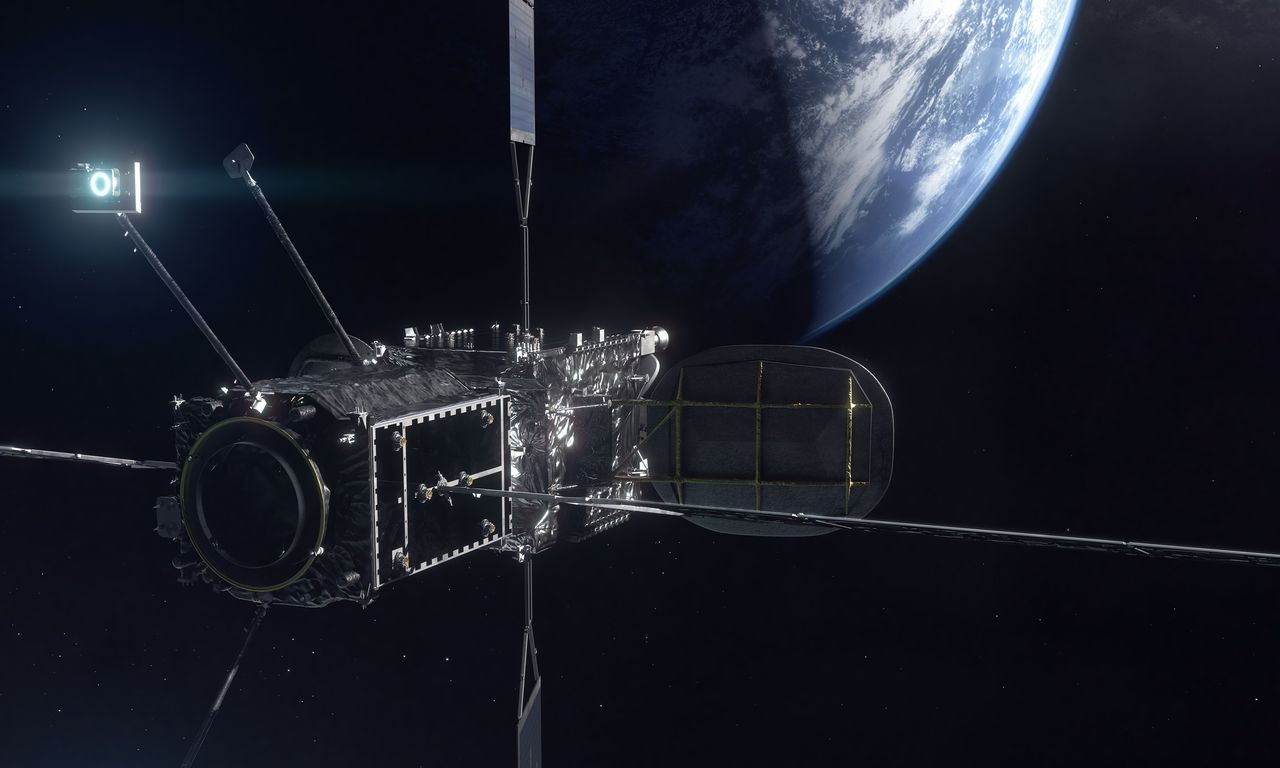
\includegraphics[width = 5.5in]{Figures/mev_ng.jpg}
		\label{Figure: Title Graphic}
		\end{figure}
        \        
        
        \Large
        AA 279D - Spacecraft Formation-Flying and Rendezvous\\
        Stanford University\\
        
    \end{center}
\end{titlepage}

% Update the revision history with each assignment
\section*{Revision History}
\begin{table}[ht]
    \centering
    % \caption{Summary of project revisions.}
    \begin{tabular}{lp{0.8\linewidth}}
        \toprule
        \textbf{Rev} & \textbf{Changes} \\
        \hline
        PS1 & \tabitem Created document \\
            & \tabitem Added problem set 1 material  \\
        \hline
        PS2 & \tabitem Added problem set 2 material  \\
            & \tabitem Added secondary mission objectives to 1.1 \\
            & \tabitem Bolded the appropriate vectors in relative orbit elements equation \\
            & \tabitem Added details on quasi-nonsingular orbit elements to Keplerian orbit elements \\
            & \tabitem Added details on Keplerian orbit elements to ECI position and velocity \\
            & \tabitem Added details on integration method \\
            & \tabitem Revised equations \ref{eq:eci2rtn} and \ref{eq:v_rtn} to specify the SV number, and change wording to highlight that we are looking at the chief's RTN frame \\
            & \tabitem Clarified wording about RTN in section \ref{sec:analytical_and_eci2rtn}. \\
            & \tabitem Fixed x-axis on Figures \ref{fig:rtn_compare_large_timestep} and \ref{fig:rtn_compare_small_timestep}. \\
            & \tabitem Added reference to Brower's Theory in section \ref{sec:comp_issues}. \\
            & \tabitem Propagated J2 orbit for more orbits to illustrate the argument of periapsis change in section \ref{sec:fode_simulation}. \\
            & \tabitem Updated reasoning behind periodic behavior in specific mechanical energy in section \ref{sec:oe_compares}. \\
        \hline
        PS3 & \tabitem Added problem set 3 material \\
        \hline
        PS4 & \tabitem Added problem set 4 material \\
        & \tabitem Minor word corrections in earlier PSets \\
        \hline
        PS5 & \tabitem Added problem set 5 material \\
        \hline
        PS6 & \tabitem Added problem set 6 material \\
        & \tabitem Plots for problem set 5 have been updated with a new sim that does both maneuvers and station keeping, but the text content is yet to be updated. 
    \end{tabular}
    \label{table:revision history}
\end{table}

\newpage
\tableofcontents

\newpage
\listoffigures

\newpage
\listoftables

%%%%%%%%%%%%%%%%%%%%%%%%%%%%%%%
% SCOPE 
%%%%%%%%%%%%%%%%%%%%%%%%%%%%%%%
\newpage
\section{Scope}
This report covers the requirements for AA279D Spacecraft Formation Flying and Rendezvous project.

%%%%%%%%%%%%%%%%%%%%%%%%%%%%%%%
% PROBLEM SETS
%%%%%%%%%%%%%%%%%%%%%%%%%%%%%%%
\section{Problem Set 1}
\subsection{Your Mission, Your Challenge}

We conducted an in-depth survey of existing and proposed Distributed Space Systems, and decided on a fictional concept consisting of a swarm performing in-orbit servicing. We are calling this fictional mission SOSS: Servicing and Observing Satellite Swarm. The goal of the mission is to have two unique satellites observe and operate on an existing satellite (called the \textbf{Target}) that needs to be serviced. The two satellites in the mission are called the \textbf{Watcher} and the \textbf{Docker}. The Watcher's objective is to observe the other two satellites and provide relative navigation information. The Docker's objective is to rendezvous with the Target and provide services such as in-space refueling and robotic servicing.

We are using Starling \cite{krugerorbit} as a baseline for numerical values for initial orbital configurations, and for swarm behavior in future assignments. We are also interested in the application of relative optical navigation, demonstrated by Starling, for our mission.

\subsubsection{Mission Name and Operator}
We are designing a mission called \textbf{SOSS}: \textbf{S}ervicing and \textbf{O}bserving \textbf{S}atellite \textbf{S}warm. Operated by the Chigullapalli-Bogdanowitsch Space Agency (CBSA)

\subsubsection{Primary and Secondary Mission Objectives}
\begin{itemize}
    \item Primary objective is to service and extend the mission lifetime of an existing Target satellite.
    \item Secondary objectives include:
    \begin{itemize}
        \item Demonstrating in-orbit relative visual navigation for spacecraft rendezvous.
        \item Demonstrating centimeter-level accuracy position control of docking spacecraft to meet servicing requirements.
        \item Demonstrating convex trajectory optimization methods for real-time generation of safe and dynamically feasible rendezvous trajectories.
    \end{itemize}
\end{itemize}
    
\subsubsection{Number and Type of Satellites}
3 satellites in the swarm. SV1 is the Target, and is the satellite we are servicing. SV2 is the Watcher, equipped with vision sensors. SV3 is the Docker, responsible for docking and equipped with servicing equipment (robotic arm, propellant tanks).

\subsubsection{Absolute Orbit Parameters}
Inherited from the Starling mission \cite{krugerorbit}, the quasi-nonsingular absolute orbit parameters of SV4 of the Starling swarm are as follows:
\begin{table}[h]
\centering
\begin{tabular}{cccccc} \hline
    $a$ & $e_x$ & $e_y$ & $i$ & $\Omega$ & $u$ \\ \hline 
     6944 km & -0.00004 & 0.0016 & 99.4 $^\circ$ & -151.1$^\circ$ & -47.9$^\circ$ \\ \hline
\end{tabular}
\caption{Absolute Orbit Parameters}
\label{tab:abs_oe}
\end{table}

We will take these parameters to be our Target SV1. 

The quasi-nonsingular absolute orbit is given by D'Amico \cite{damicothesis} as:
\begin{align}
\boldsymbol{\alpha} &= 
\begin{bmatrix}
a & e_x & e_y & i & \Omega & u
\end{bmatrix}^\top \notag \\
&= 
\begin{bmatrix}
a & e \cos \omega & e \sin \omega & i & \Omega & \omega + M
\end{bmatrix}^\top
\end{align}

where $a, e, i, \Omega, \omega, M$ are the Keplerian orbit elements. These are converted to standard Keplerian orbital elements in Section \ref{sec:initial_oe}.

\subsubsection{Relative Orbit Parameters}\label{sec:ROE_init}
Again, inheriting from the Starling mission, the quasi-nonsingular relative orbit elements (ROE) of SV3 and SV2 with respect to SV4 are given by the following. These parameters, along with the absolute ones, occurred at 02/05/24 00:00:00 UTC, but we will define them as our starting parameters at an arbitrary point in the future: 
\begin{table}[h!]
\centering
\begin{tabular}{ll}
\toprule
\textbf{ID} & \textbf{In-Train Formation} \\
\midrule
SV2 & $\delta\boldsymbol{\alpha} = [21, -124350, 110, 202, 79, 1005]~\text{m}$ \\
SV3 & $\delta\boldsymbol{\alpha} = [-1, -79328, 42, 452, 36, 827]~\text{m}$ \\
\bottomrule
\end{tabular}
\caption{Quasi-Nonsingular Relative Orbit Parameters}
\label{tab:relative_oe}
\end{table}

We will take the Starling SV4 to be our Target SV1, the Starling SV2 to be our Watcher SV2, and Starling SV3 to be our Docker SV3. 

The quasi-nonsingular ROE adopted by D'Amico \cite{damicothesis} are a function of the orbit elements of the target $t$ and observer $o$. They are given by:
\begin{align}
\delta \boldsymbol{\alpha} &= 
\begin{bmatrix} \label{eq:quasi_nonsign_roe}
\delta a & \delta \lambda & \delta e_x & \delta e_y & \delta i_x & \delta i_y
\end{bmatrix}^\top \notag \\
&= 
\left( 
\begin{bmatrix}
\delta a \\
\delta \lambda \\
|\delta\mathbf{e}| \cos \phi \\
|\delta\mathbf{e}| \sin \phi \\
|\delta\mathbf{i}| \cos \theta \\
|\delta\mathbf{i}| \sin \theta
\end{bmatrix}
= 
\begin{bmatrix}
\frac{a_t - a_o}{a_o} \\
(u_t - u_o) + (\Omega_t - \Omega_o) \cos i_o \\
e_{x,t} - e_{x,o} \\
e_{y,t} - e_{y,o} \\
i_t - i_o \\
(\Omega_t - \Omega_o) \sin i_o
\end{bmatrix}
\right)
\end{align}

where $[\delta e_x, \delta e_y]$ are components of the relative eccentricity vector with phase $\phi$ and $[\delta i_x, \delta i_y]$ are components of the relative inclination vector with phase $\theta$.    

\subsubsection{Launch Date and Mission Duration} 
May 8th, 2031; 6 month mission duration.

\subsubsection{Key DGN\&C requirements}


The swarm and rendezvous requirements for the Watcher, Docker, and the relation between those satellites and the Target are given as (and inspired again by the requirements for the Starling mission \cite{kruger2024starling}):

\begin{itemize}
    \item The inter-satellite distance between the Watcher and the Docker shall not exceed the limit for inter-satellite communication.
    \item The Watcher shall have the Target in its camera's field of view at all times 
    \item The Watcher shall maintain a safe inter-satellite distance to the Docker and Target, on the order of $\approx100$ meters, at all times.
    \item The Watcher's bearing angle measurements of the Target/Docker shall not remain constant.
    \item When not in the final docking phase, the Docker shall maintain a safe inter-satellite distance to the Target on the order of $\approx 100$ meters.
    \item During the docking phase, the Docker shall compute a fuel-optimal rendezvous trajectory to the Target.
    \item The Docker shall track the optimal rendezvous trajectory to $\approx 10 cm$ accuracy when in close-proximity to the Target.
    \item The Watcher shall provide a relative position measurement of the Docker/Target around the $\approx 10 cm$ accuracy.
    \item During the docking phase, the Watcher shall have both the Target and Docker in its camera's field of view.
    \item All satellites shall stay in a stable low-earth orbit for the entirety of the mission.
\end{itemize}


\subsubsection{Classification of DSS} 
Our mission will be a Swarm that involves Rendezvous and Docking. We classify this mission as a swarm based on the small inter-satellite separation when orbiting close to the Target satellite and the high navigation accuracy required in such a situation. The mission is also a Rendezvous and Docking mission because the requirements have the Docker and Target docking.

\subsection{Orbit Simulation, Review of Astrodynamics}
\subsubsection{Initial Orbital Elements} \label{sec:initial_oe}
The initial conditions are taken from the Starling mission literature \cite{krugerorbit} and are provided in Table \ref{tab:abs_oe}. These elements, originally provided in the quasi-nonsingular absolute orbit parameters, were first converted to the Keplerian orbital elements, which are given in Table \ref{tab:abs_oe_kepler}.

\begin{table}[h]
\centering
\begin{tabular}{cccccc} \hline
    $a$ & $e$ & $i$ & $\omega$ & $\Omega$ & $\nu$ \\ \hline 
     6944 km & 0.0016 & 99.4 $^\circ$ & 91.432$^\circ$ & -151.1$^\circ$ & -139.45$^\circ$ \\ \hline
\end{tabular}
\caption{Inital Keplerian Orbit Parameters of SV1}
\label{tab:abs_oe_kepler}
\end{table}

For future use, it is also useful to note that the corresponding initial mean anomaly $M_0= -139.33^\circ$.

The quasi-nonsingular absolute orbit parameters were converted to the Keplerian orbital elements by using the following procedure. First, compute the argument of perigee, eccentricity, and the mean anomaly:
\begin{align}
\omega = \tan^{-1} \left( \frac{e_y}{e_x} \right)
e = \frac{e_x}{\cos \omega}
M = u - \omega
\end{align}

Then, convert mean anomaly to radians and solve Kepler's equation using Newton-Raphson to obtain eccentric anomaly \( E \).

Finally, compute the true anomaly:
\begin{align}
\nu = \tan^{-1} \left( \frac{\sqrt{1 + e} \cdot \tan(E/2)}{\sqrt{1 - e}} \right) \cdot 2
\end{align}

\subsubsection{Initial Position and Velocity in ECI}\label{sec:initial_ECI}
 Treating the initial Keplerian orbital elements for the target SV1 given in Table \ref{tab:abs_oe_kepler} as osculating quantities, they can be converted into Earth-Centered Inertial (ECI) position (in km) and velocity (in km/s), and are 
 \begin{align} \label{eq:SV1_initial_ECI}
     \boldsymbol{r}_{0, ECI, SV1} &= \begin{bmatrix}
         -3663.3 \\
         -2986.4 \\
         -5098.8
     \end{bmatrix} \\
     \boldsymbol{v}_{0, ECI, SV1} &= \begin{bmatrix}
         -5.3201 \\
         -1.9915 \\
         4.9994
     \end{bmatrix}.
 \end{align}

The conversion from Keplerian orbital elements to ECI position and velocity is as follows. First, we calculate norm of the position $r$:

\begin{align}
r = \frac{a(1 - e^2)}{1 + e \cos \nu}
\end{align}

And then transform it into the PQW (perifocal) frame:
\begin{align}
\mathbf{r}_{PQW} = \begin{bmatrix}
r \cos \nu \\
r \sin \nu \\
0
\end{bmatrix}
\end{align}

Next we compute mean motion:
\begin{align}
n = \sqrt{\frac{\mu}{a^3}}
\end{align}

And then we compute the eccentric anomaly:
\begin{align}
E = 2 \cdot \tan^{-1} \left( \sqrt{\frac{1 - e}{1 + e}} \cdot \tan\left(\frac{\nu}{2}\right) \right)
\end{align}

The rotation matrix from PQW to ECI (IJK) frame is given by:
\begin{align}
R_{\text{PQW} \to \text{ECI}} = 
\begin{bmatrix}
\cos\Omega\cos\omega - \sin\Omega\cos i\sin\omega & -\cos\Omega\sin\omega - \sin\Omega\cos i\cos\omega & \sin\Omega\sin i \\
\sin\Omega\cos\omega + \cos\Omega\cos i\sin\omega & -\sin\Omega\sin\omega + \cos\Omega\cos i\cos\omega & -\cos\Omega\sin i \\
\sin i\sin\omega & \sin i\cos\omega & \cos i
\end{bmatrix}
\end{align}

And the velocity in PQW frame is:
\begin{align}
\mathbf{v}_{PQW} = \frac{a n}{1 - e \cos E}
\begin{bmatrix}
-\sin E \\
\sqrt{1 - e^2} \cos E \\
0
\end{bmatrix}
\end{align}

Finally, we can transform to the ECI frame:
\begin{align}
\mathbf{r}_{ECI} = R_{\text{PQW} \to \text{ECI}} \cdot \mathbf{r}_{PQW}
\qquad
\mathbf{v}_{ECI} = R_{\text{PQW} \to \text{ECI}} \cdot \mathbf{v}_{PQW}
\end{align}

\subsubsection{Numerical Simulation of State with Perturbations} \label{sec:fode_simulation}
The state of the satellite is represented by 
\begin{align}
    \boldsymbol{x} = \begin{bmatrix}
        \boldsymbol{r}^T & \boldsymbol{v}^T
    \end{bmatrix}^T
\end{align}

The derivative of this state is given by 
\begin{align}
    \boldsymbol{\dot{x}} = \begin{bmatrix}
        \boldsymbol{v}^T & \boldsymbol{a}^T
    \end{bmatrix}^T
\end{align}

where $a$ is the acceleration on the satellite from the primary attractor. The acceleration due to gravity is given by
\begin{align}
    \boldsymbol{a_g} = \frac{-\mu}{||\boldsymbol{r}||^3} \boldsymbol{r}.
\end{align}

The additional J2 perturbation acceleration vector is given by 

\[
\mathbf{a}_{J2} = \frac{3 J_2 \mu R_e^2}{2 r^5} \begin{bmatrix}
\left(5\frac{r_z^2}{r^2} - 1\right) r_x \\
\left(5\frac{r_z^2}{r^2} - 1\right) r_y \\
\left(5\frac{r_z^2}{r^2} - 3\right) r_z
\end{bmatrix}
\]

Then the total acceleration when including J2 is

\[
\mathbf{a} = \mathbf{a}_{\text{g}} + \mathbf{a}_{J2}
\]

With these acceleration terms, we can propagate the state through an integer number of orbits (25 in our case) and obtain the orbital path. We used a custom Runge-Kutta (RK4) integrator with a fixed step size of $\frac{1}{500}$ of the orbit period to ensure accuracy. This choice is validated by the analysis in Section \ref{sec:analytical_and_eci2rtn}.

\begin{align}
    t_{orbit} = 2\pi \sqrt{\frac{a_0^3}{\mu_{earth}}} \\
    t_{total} = 25t_{orbit} \\
    \Delta t = \frac{t_{orbit}}{500} \label{eq:timestep}% Time step (s)
\end{align}

Figure \ref{fig:3d_plots_with_j2} shows the 3D plot of the orbit in an inertial frame, and compares the orbit with and without J2 perturbations, but propagated for 200 orbits to illustrate the change in the argument of periapsis. 

\begin{figure}[H]
    \centering
    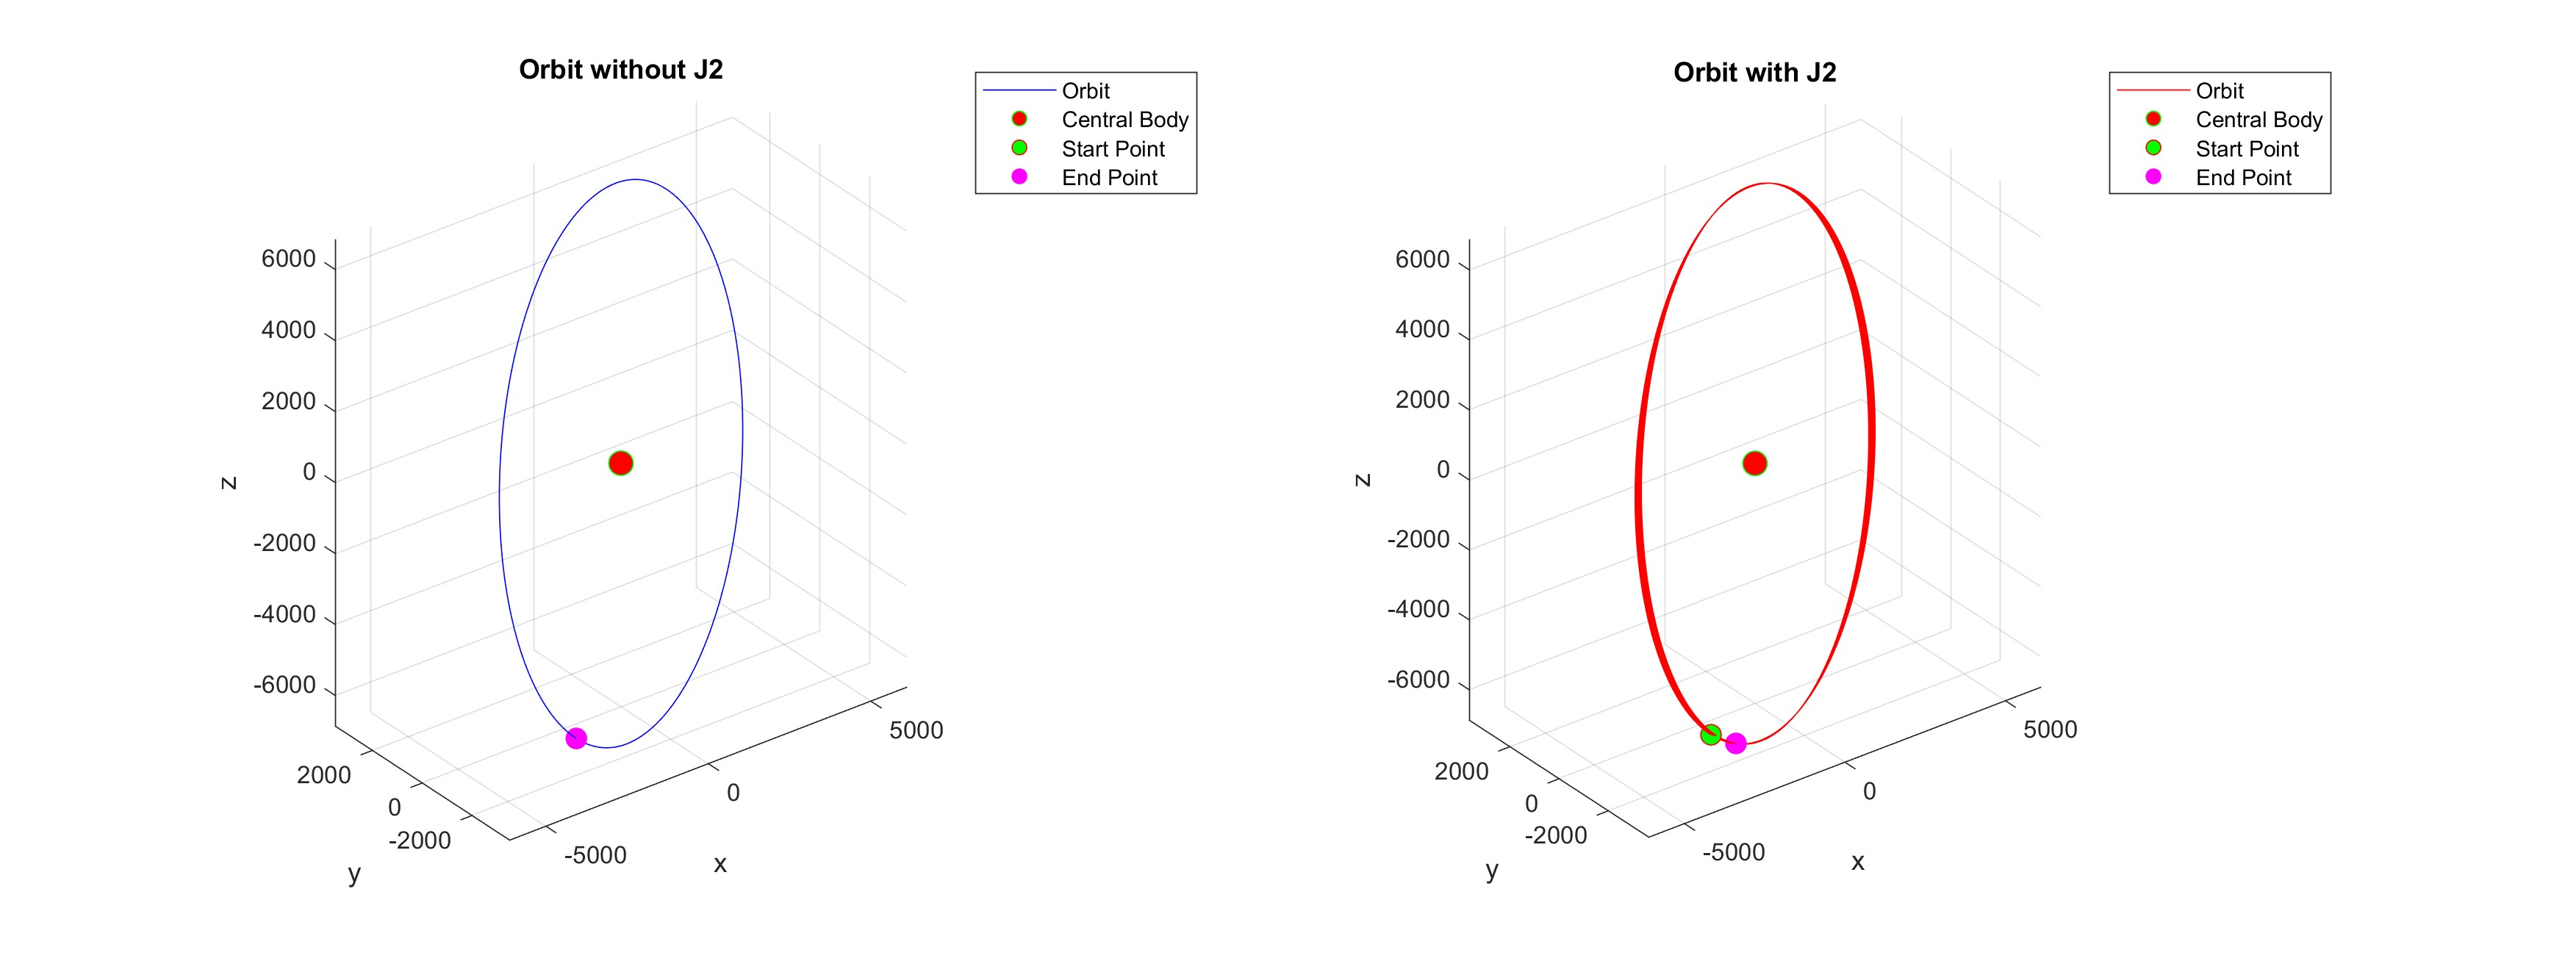
\includegraphics[width=1.1\linewidth]{PS1/Figures/Orbit_J2_Comparison_ECI.jpg}
    \caption{Comparison of the 3D plots with (right) and without (left) J2 perturbations. }
    \label{fig:3d_plots_with_j2}
\end{figure}

As expected, the most prominent change in the orbit with J2 perturbations is in the RAAN. The change in RAAN is secular rather than periodic, as will be seen in more detail in the plots in Section \ref{sec:oe_compares}.

\subsubsection{Comparison with Analytical Keplerian Propagation} \label{sec:analytical_and_eci2rtn}

We can compare the no-J2 simulation with the analytical Keplerian result for the orbital parameters mentioned in Table \ref{tab:abs_oe_kepler}, but by varying the true anomaly $\nu$. 

The time-steps used in the numerical propagation $t$ are converted into $\nu$ values (via intermediate computation of mean anomaly $M$ and eccentric anomaly $E$). The state outputs from both the numerical simulation and the analytical keplerian solution are converted from the ECI frame into the Radial-Tangent-Normal (RTN) frame of the chief (SV1).

The rotation matrix from ECI to RTN of the chief is done as follows:

\begin{align}
    \boldsymbol{\hat{R}} &= \frac{\boldsymbol{r}^{ECI}_{SV1}}{||\boldsymbol{r}^{ECI}_{SV1}||} \\ \
    \boldsymbol{\hat{N}} &= \frac{\boldsymbol{r}^{ECI}_{SV1} \times \boldsymbol{v}^{ECI}_{SV1}}{||\boldsymbol{r}^{ECI}_{SV1} \times \boldsymbol{v}^{ECI}_{SV1}||} \\
    \boldsymbol{\hat{T}} &= \boldsymbol{\hat{N}} \times \boldsymbol{\hat{R}} \\
    Q_{eci2rtn} &= \begin{bmatrix}
        \boldsymbol{\hat{R}} & \boldsymbol{\hat{T}} & \boldsymbol{\hat{N}}
    \end{bmatrix}^T \label{eq:eci2rtn}
\end{align}

From this, we calculate the RTN position $r_{RTN}$ and velocity $v_{RTN}$ to be

\begin{align}
    \boldsymbol{r}^{RTN}_{SV1} &= R_{eci2rtn} \boldsymbol{r}^{ECI}_{SV1} \\
    \boldsymbol{v}^{RTN}_{SV1} &= R_{eci2rtn} \boldsymbol{v}^{ECI}_{SV1} - \omega_{RTN} \times \boldsymbol{r}^{RTN}_{SV1} \label{eq:v_rtn}
\end{align}

where $\omega_{RTN} = \begin{bmatrix}
    0 & 0 & ||r\times v ||/||r||^2
\end{bmatrix}$ is the angular velocity of the frame. As expected, the position of the chief in its own RTN frame is only in the radial direction. With the velocity, since the frame is rotation at the same rate as the chief satellite, the velocity in the RTN frame is nearly zero (apart from a small radial component because of the eccentricity of the orbit). If the orbit was more eccentric, there would be a larger radial component.

In the absence of numerical errors, the results from the numerical simulation and Keplerian solution should match. However, with larger time-steps, the numerical error in the numerical propagator increases. Figure \ref{fig:rtn_compare_large_timestep} shows the increasing numerical error in the position and velocity vectors when using a large time-step (only 50 steps per orbit). On the other hand, if we use a smaller time-step so that we have 500 steps per orbit, then the numerical error is much more contained, as can be seen in Figure \ref{fig:rtn_compare_small_timestep}. Since the tangential and normal components are zero in the RTN frame for both the numerical propagator and the Keplerian propagator, the error in those is also just noise.

\begin{figure}[H]
    \centering
    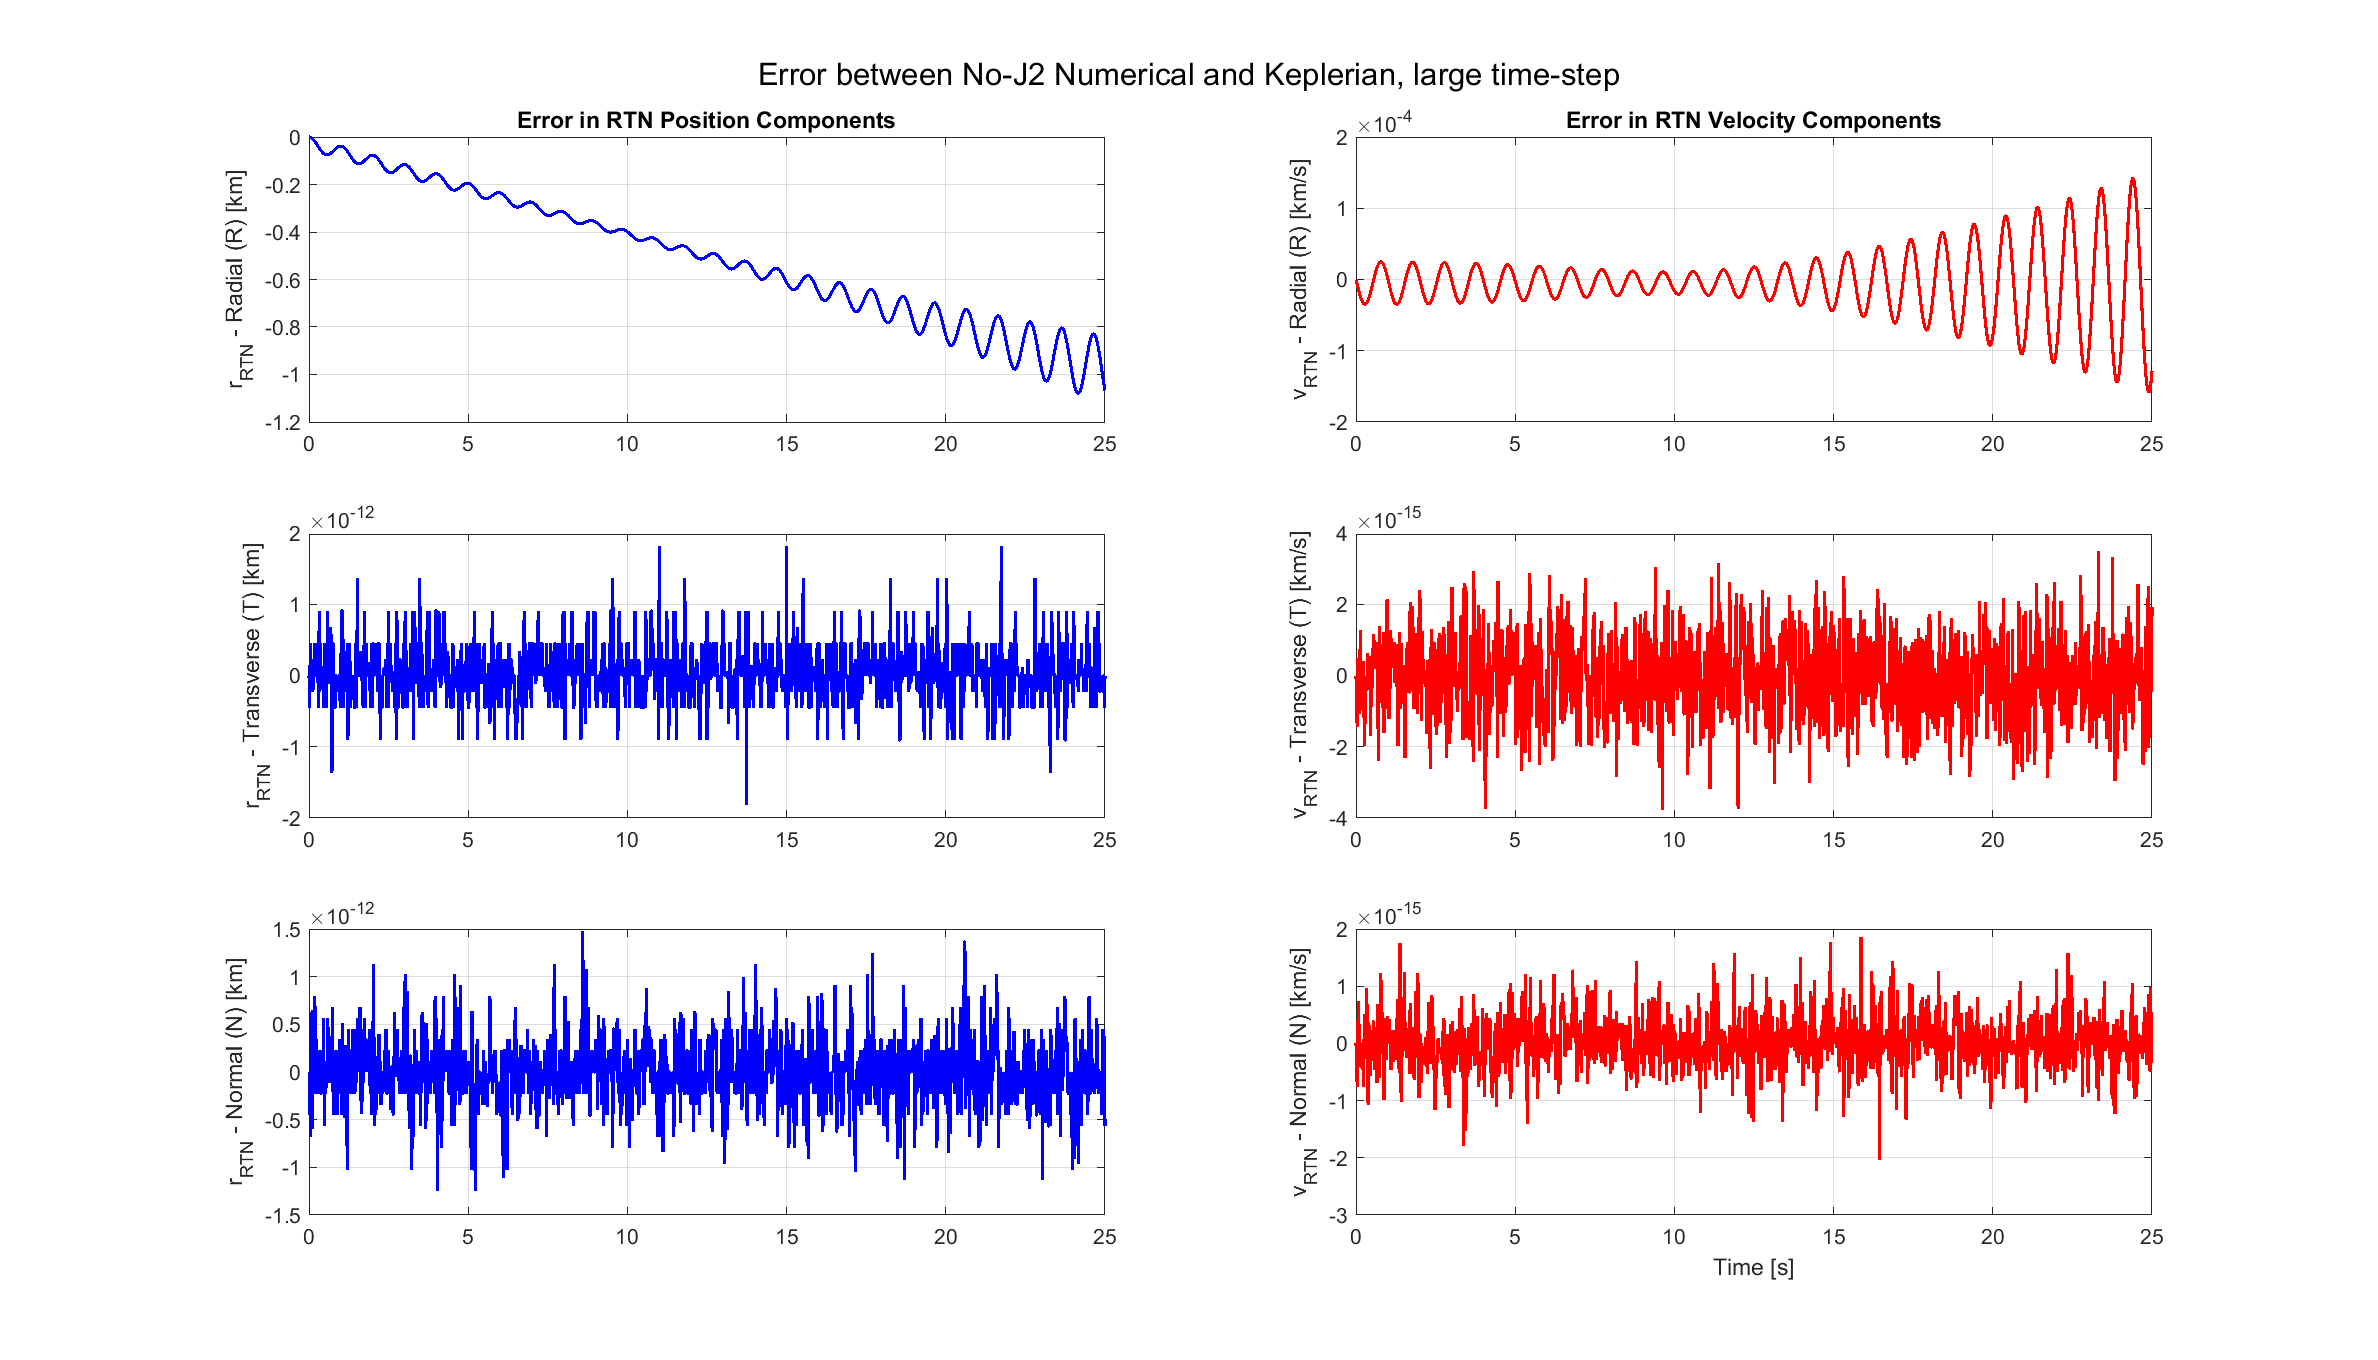
\includegraphics[width=0.75\linewidth]{sim/figures/comparing_rtn_large_timestep.png}
    \caption{Error in RTN position and velocity, with the large time-step (50 steps per orbit)}
    \label{fig:rtn_compare_large_timestep}
\end{figure}

\begin{figure}[H]
    \centering
    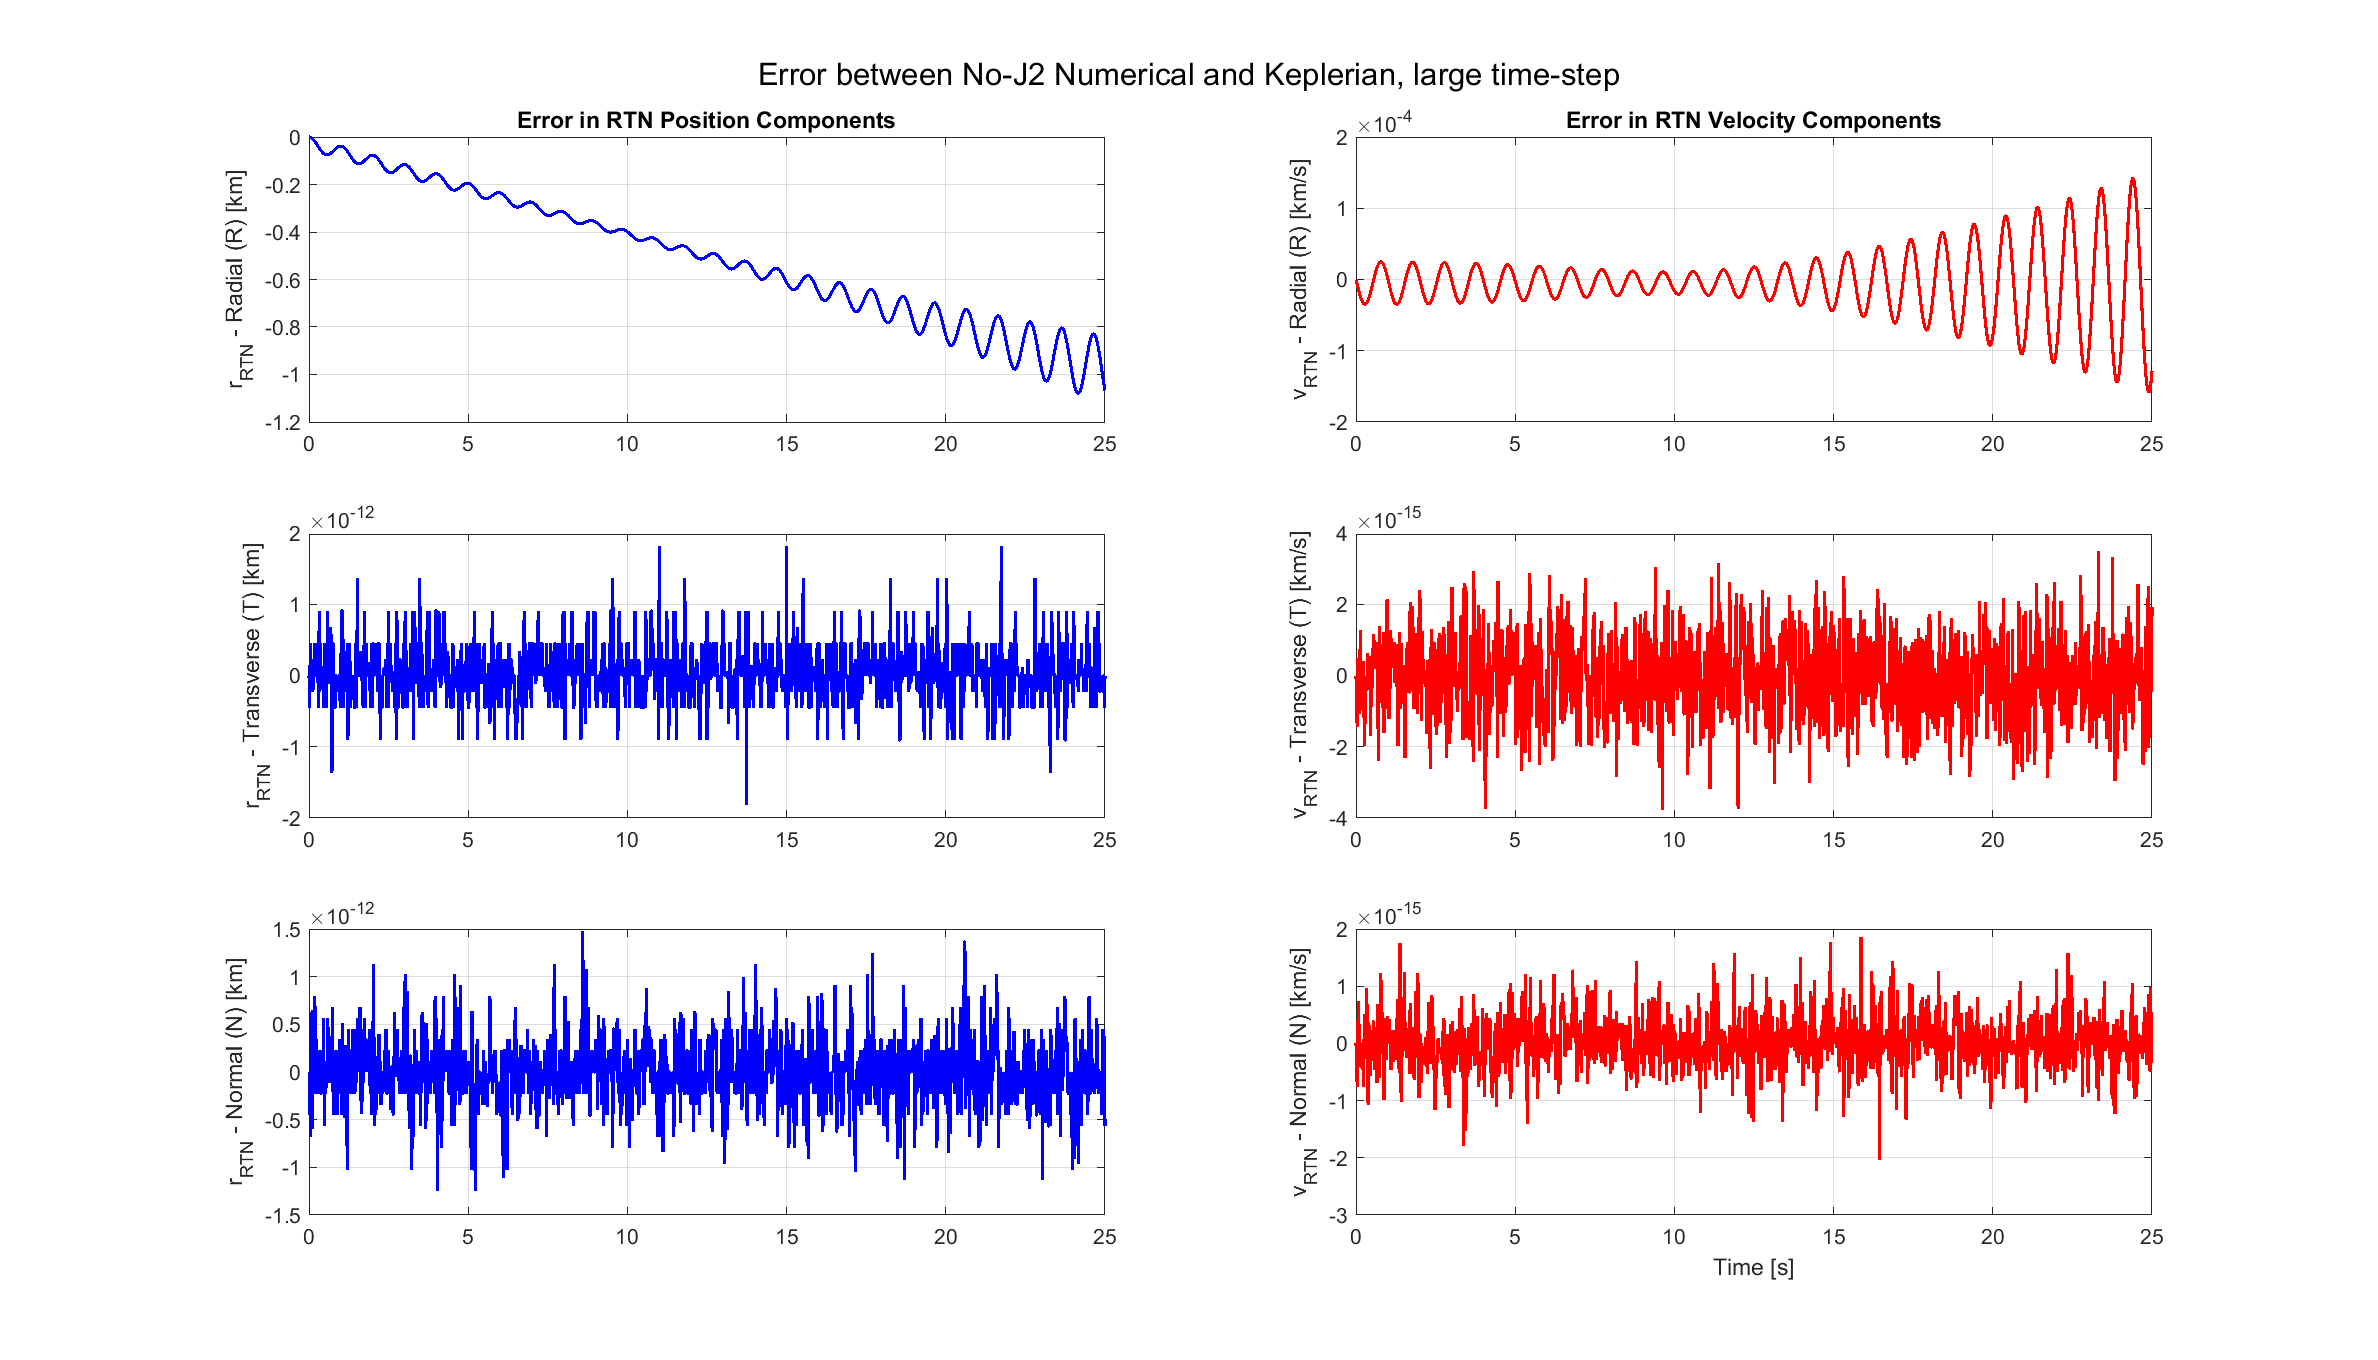
\includegraphics[width=0.75\linewidth]{sim/figures/comparing_rtn_large_timestep.png}
    \caption{Error in RTN position and velocity, with the small time-step (500 steps per orbit)}
    \label{fig:rtn_compare_small_timestep}
\end{figure}

Based on this, we can conclude that the FODE method that was used here (Fundamental Orbital Differential Equations) starts to accumulate numerical error for larger time-steps. The time-step needs to be reduced to very small values to keep the numerical error from becoming a problem.

\subsubsection{Orbital Elements, Eccentricity Vector, Angular Momentum, Specific Mechanical Energy} \label{sec:oe_compares}

First we compute the osculating Keplerian orbital elements at each time step by converting from the ECI position and velocity at that time step given by our propagator. We then compute the eccentricity vector $\boldsymbol{e}$, the angular momentum vector $\boldsymbol{h}$, and the specific mechanical energy $\epsilon$, throughout the numerical simulations with and without J2 perturbations. To compute these orbital parameters we use the following relationships:

\begin{align}
    \boldsymbol{h} &= \boldsymbol{r}_{ECI} \times \boldsymbol{v}_{ECI} \\
    \boldsymbol{e} &= \frac{\boldsymbol{v}_{ECI} \times \boldsymbol{h}}{\mu_{earth}} - \frac{\boldsymbol{r}_{ECI}}{||\boldsymbol{r}_{ECI}||} \\
    \epsilon &= \frac{||\boldsymbol{v}_{ECI}||^2}{2} - \frac{\mu_{earth}}{||\boldsymbol{r}_{ECI}||}
\end{align}

Figure \ref{fig:j2_oe_comparison} shows the Keplerian orbital elements with and without J2 perturbations over 25 orbits. As expected when excluding J2 effects, all elements remain constant except true anomaly which cycles through 360 degrees. When including J2 effects, we observe periodic and secular effects on all elements, which is expected since J2 acts in all of the RTN directions. The purely periodic effects are seen in semi-major axis, eccentricity, and inclination. The amplitude of these periodic effects are relatively small, especially for inclination and eccentricity. The other three elements - RAAN, argument of periapsis, and true anomaly - experience both periodic and secular drifts, although at different rates of change. This agrees with averaging theory which says that only these three elements experience secular drifts. The largest secular drift is in the RAAN, which is expected from the expressions for average secular drifts. There is also a small but noticeable secular drift in the argument of perigee $\omega$, that also appears in true anomaly. 

\begin{figure}[H]
    \centering
    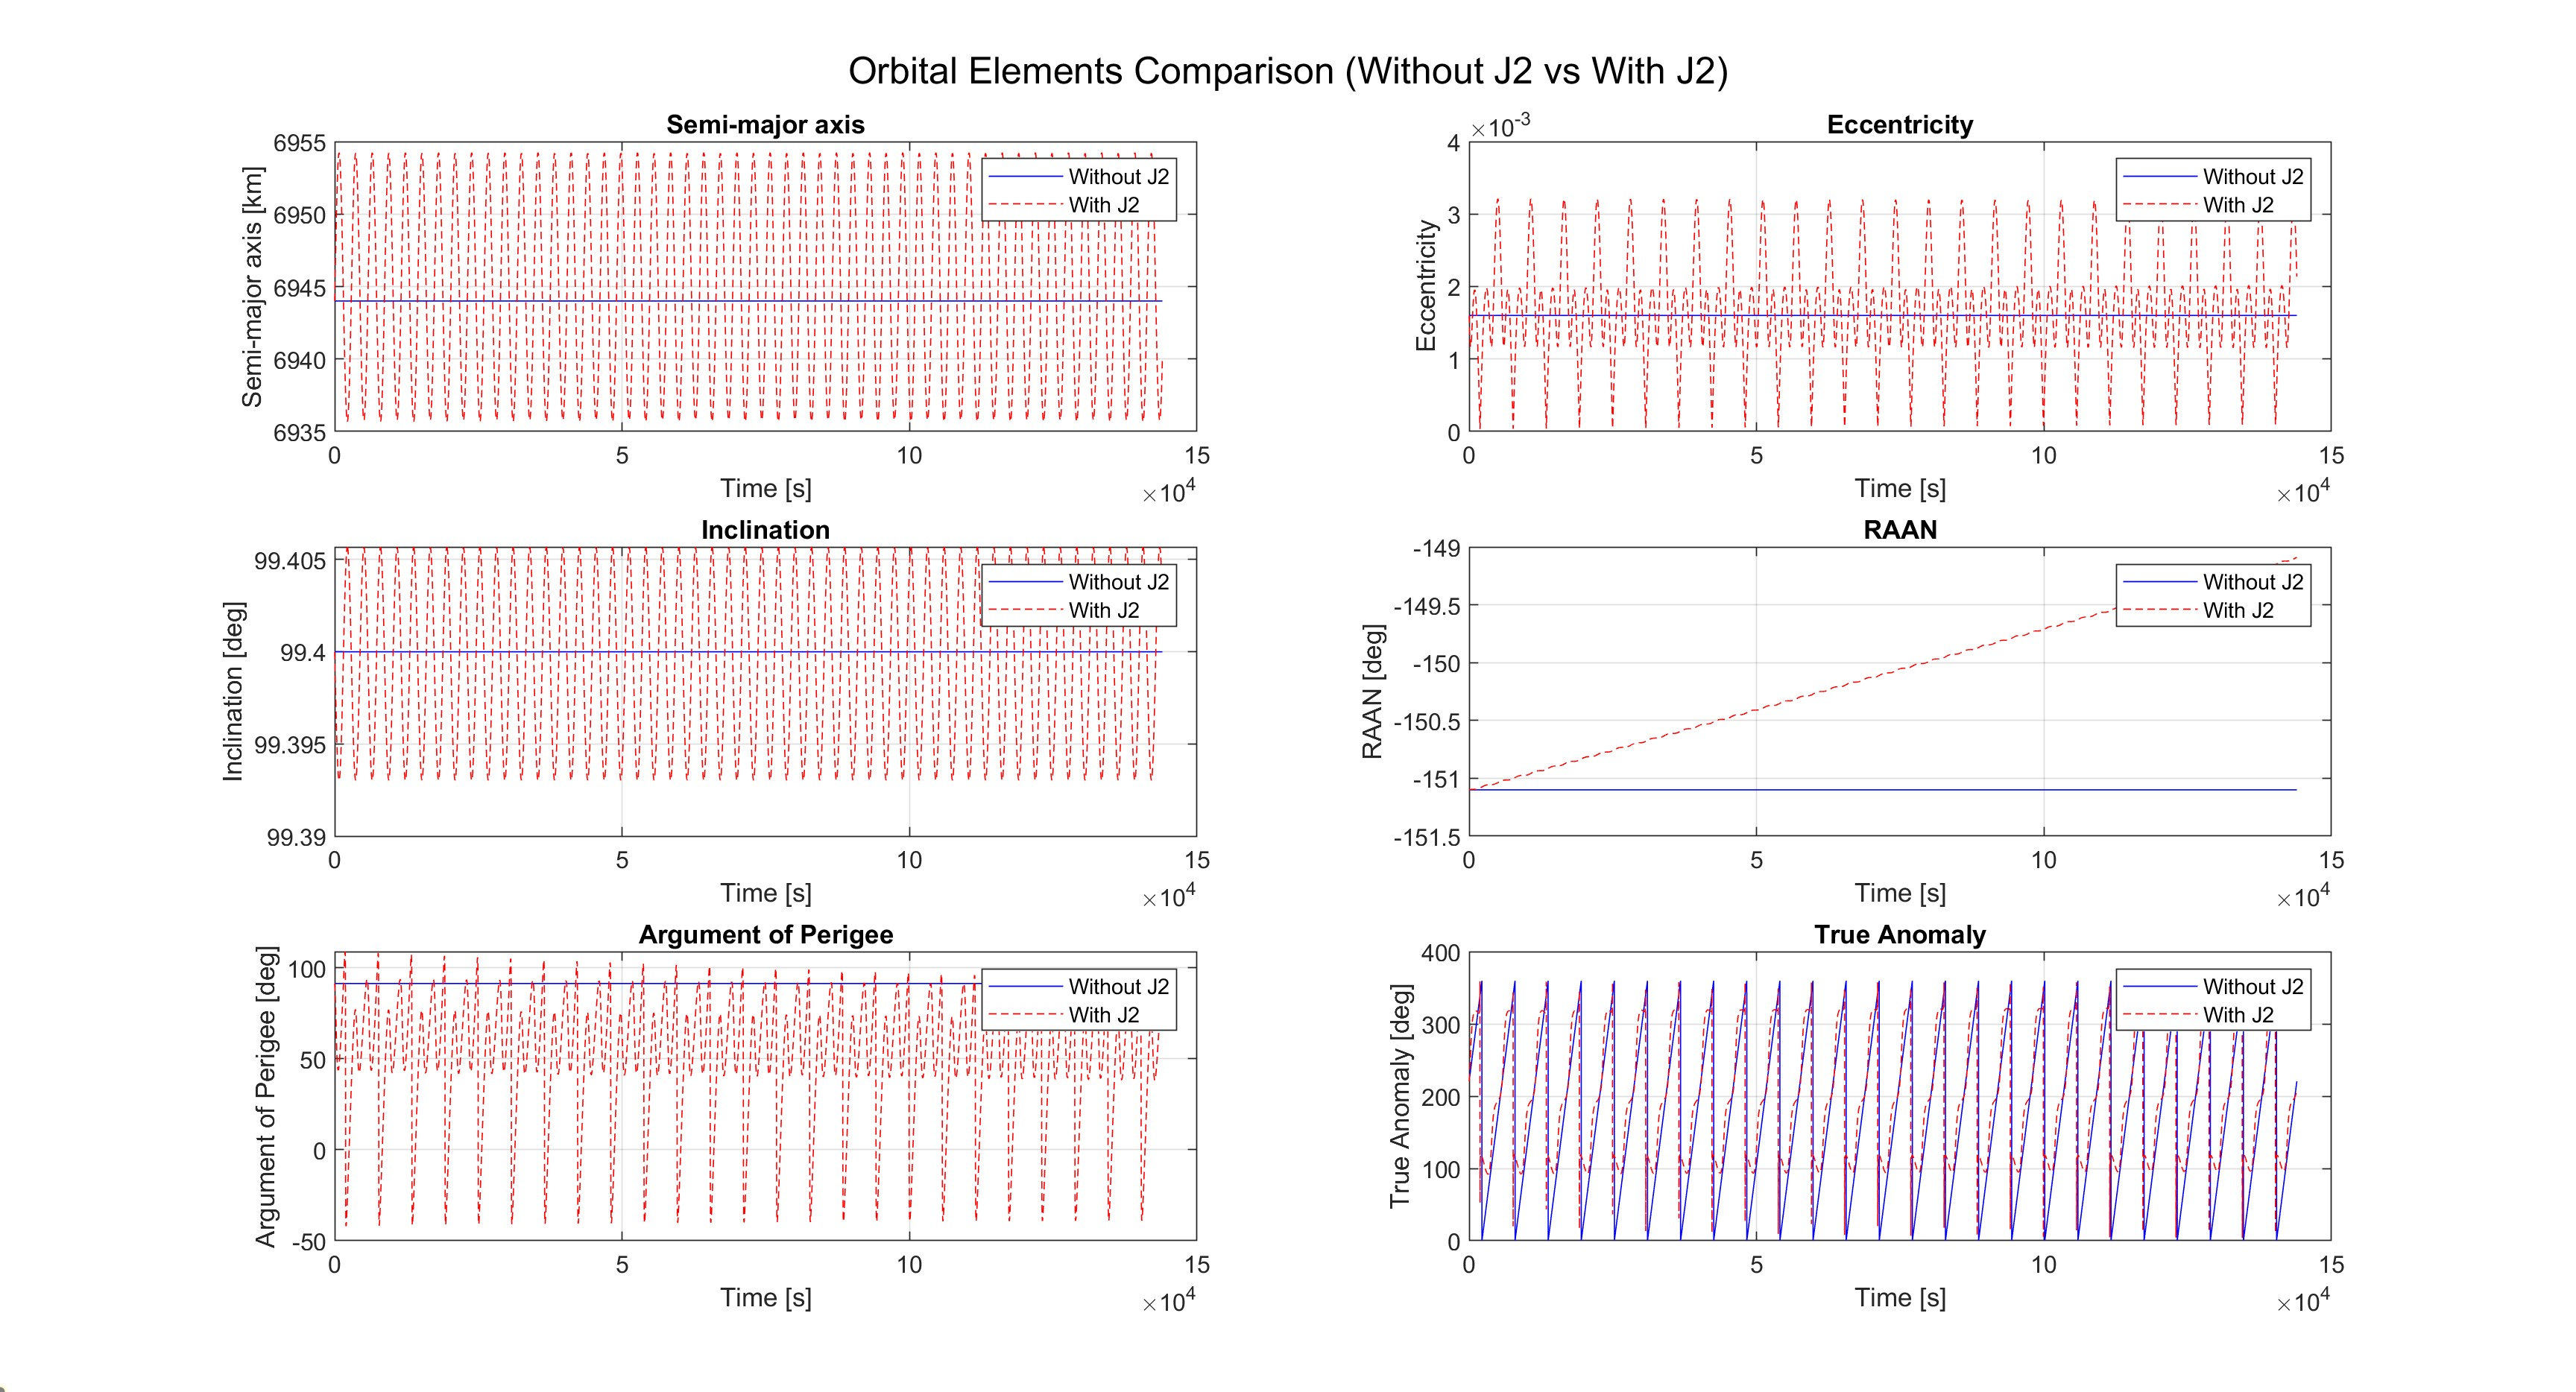
\includegraphics[width=1.1\linewidth]{PS1/Figures/OE_J2_Comparison.jpg}
    \caption{Comparison of Keplerian Orbital Elements with and without J2 perturbations over 25 orbits}
    \label{fig:j2_oe_comparison}
\end{figure}

\begin{figure}[H]
    \centering
    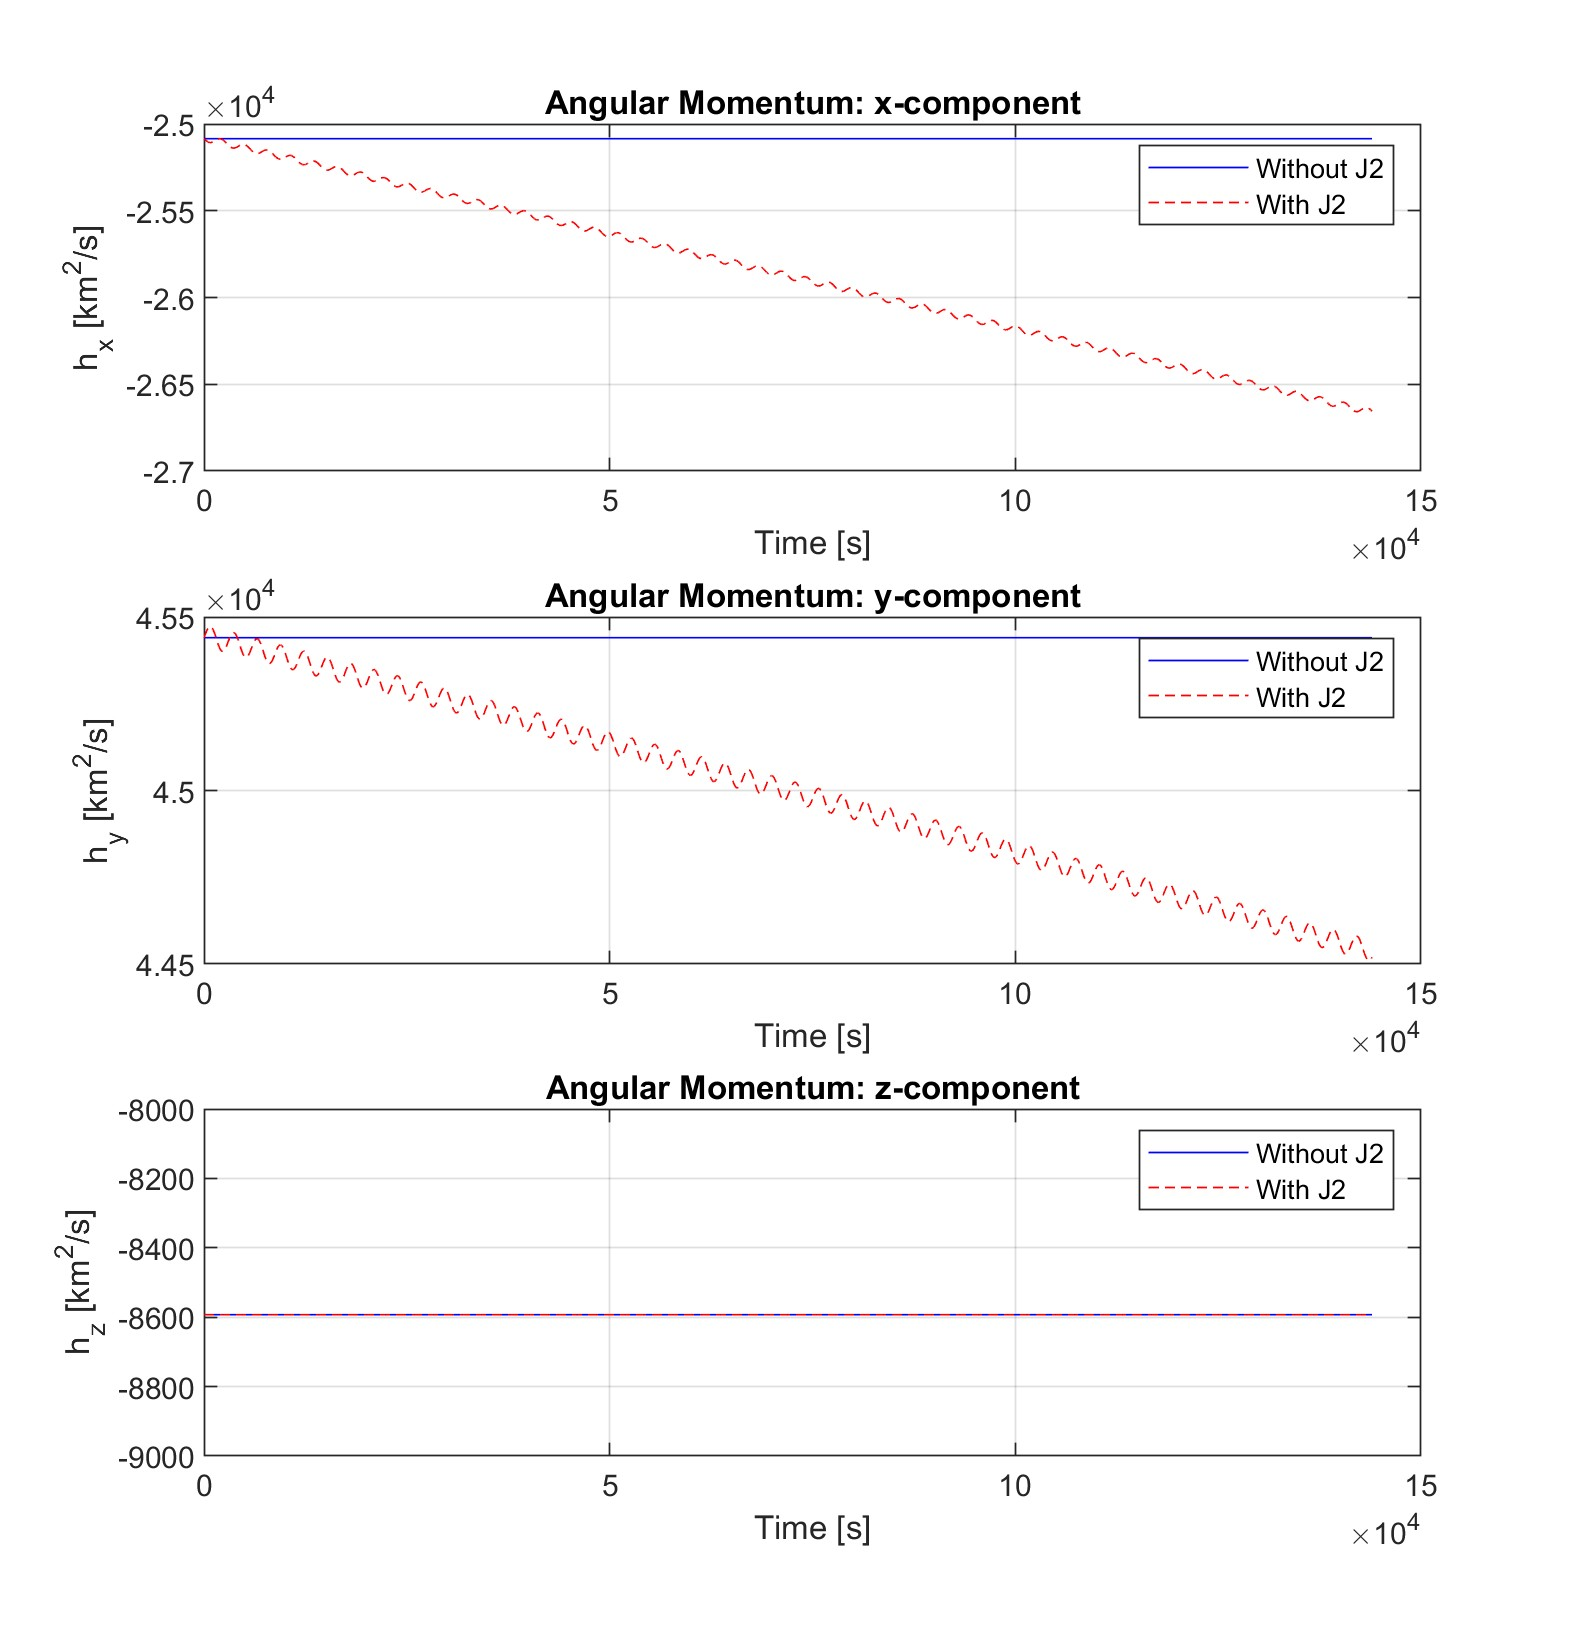
\includegraphics[width=0.5\linewidth]{PS1/Figures/h_J2_comparison.jpg}
    \caption{Comparison of Angular Momentum Vector with and without J2 perturbations over 25 orbits}
    \label{fig:angular_momentum}
\end{figure}

Figure \ref{fig:angular_momentum} compares the angular momentum vector over 25 orbits with and without J2. As expected without J2, the angular momentum vector remains constant. As expected from averaging theory, with J2 there are secular drifts in the x and y components of angular momentum. The z component remains constant because the angular velocity vector is tracing out a cone due to the effects of J2. There are also short-periodic effects on these components from J2.  

\begin{figure}[H]
    \centering
    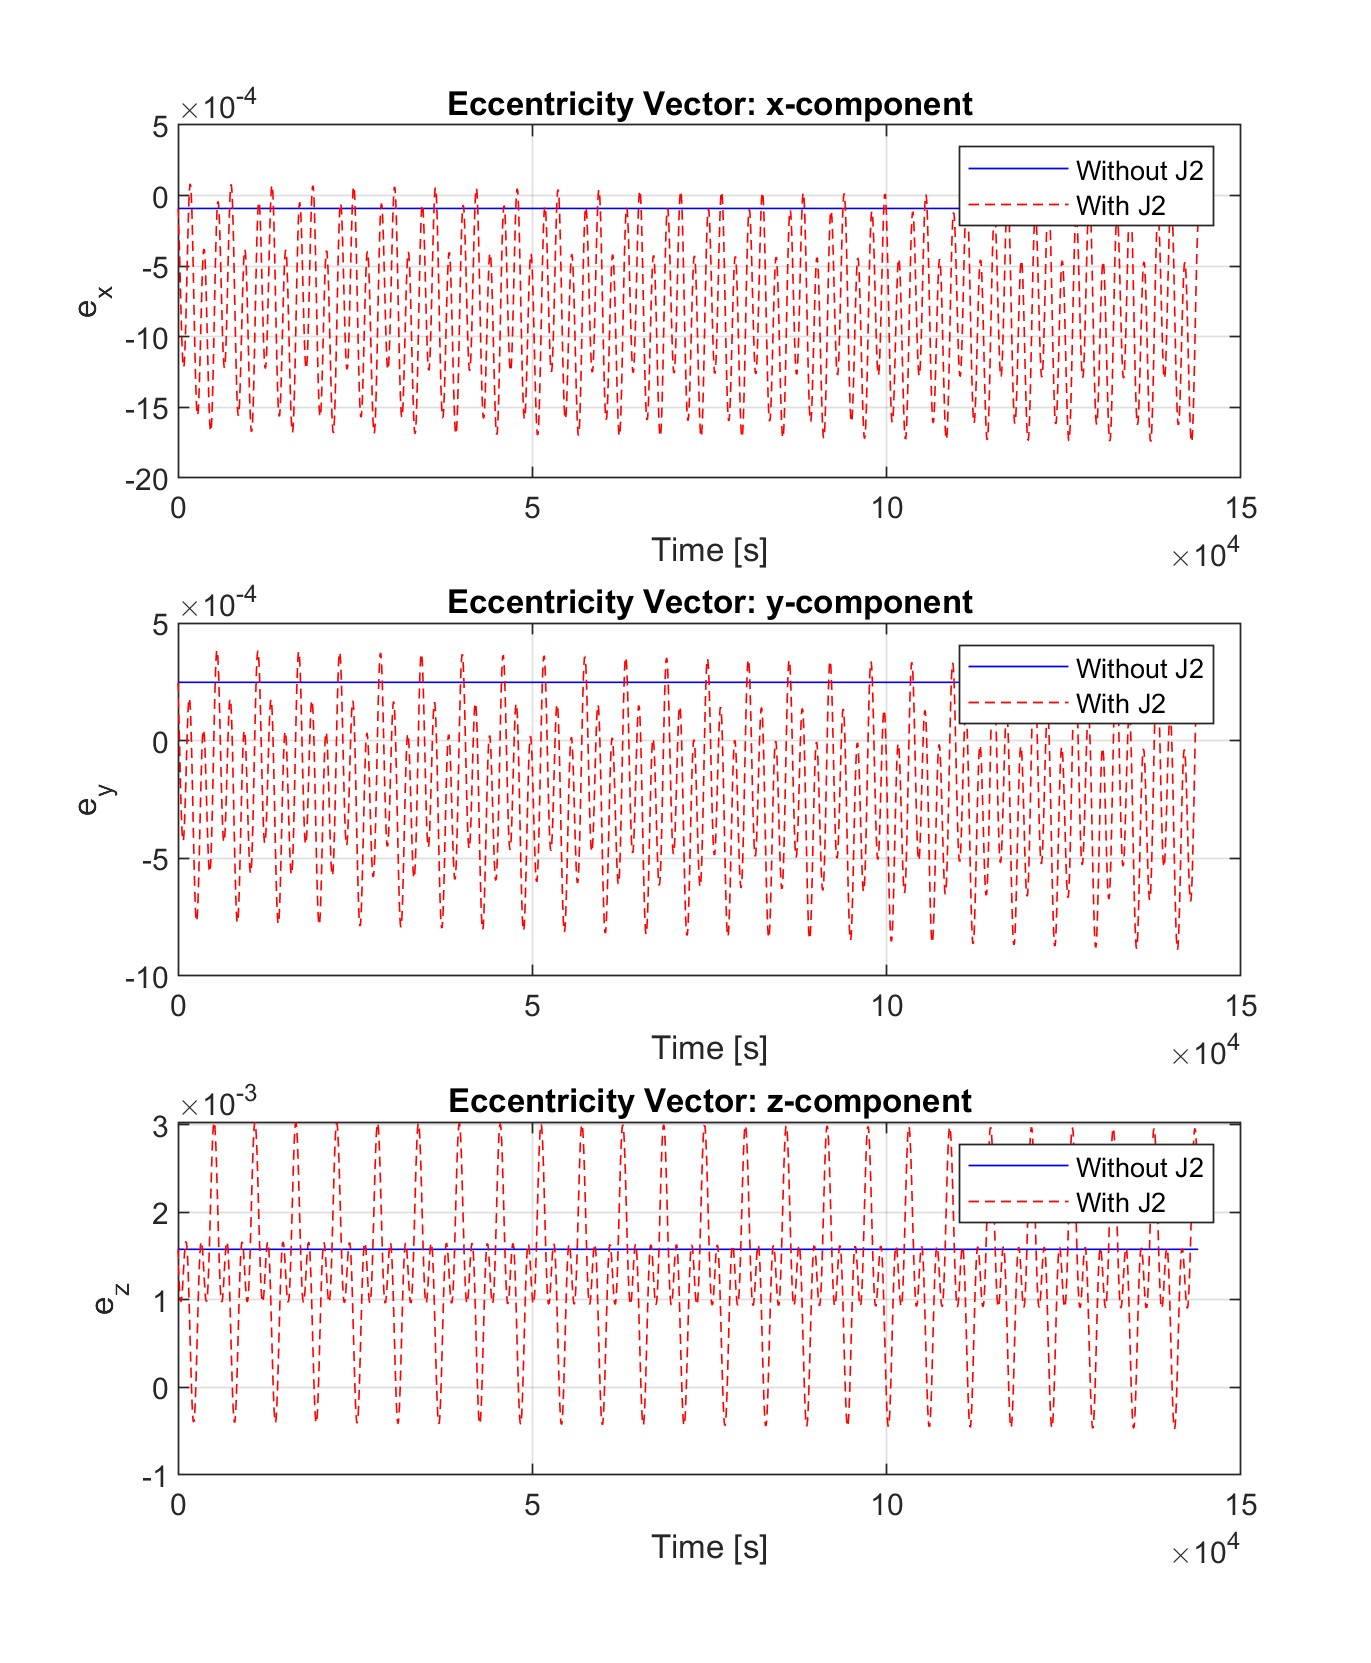
\includegraphics[width=0.5\linewidth]{PS1/Figures/ecc_J2_comparison.jpg}
    \caption{Comparison of Eccentricity Vector with and without J2 perturbations over 25 orbits}
    \label{fig:eccentricity_vector}
\end{figure}

Figure \ref{fig:eccentricity_vector} compares the eccentricity vector over 25 orbits with and without J2. As expected, without J2, the eccentricity vector remains constant. As expected from averaging theory, with J2 there are secular drifts in the x and y components of the eccentricity vector. This corresponds to the secular drift in the argument of periapsis. There are also short-periodic effects on these components from J2.  


Figure \ref{fig:specific_energy} compares the specific mechanical energy over 25 orbits with and without J2. As expected, without J2, the specific mechanical energy remains constant. With J2, the average specific mechanical energy also remains constant, which is expected since gravity is a conservative force and thus will not affect the specific mechanical energy. The periodic behavior with J2 is due to the oscillating behavior in the semi-major axis. 

\begin{figure}[H]
    \centering
    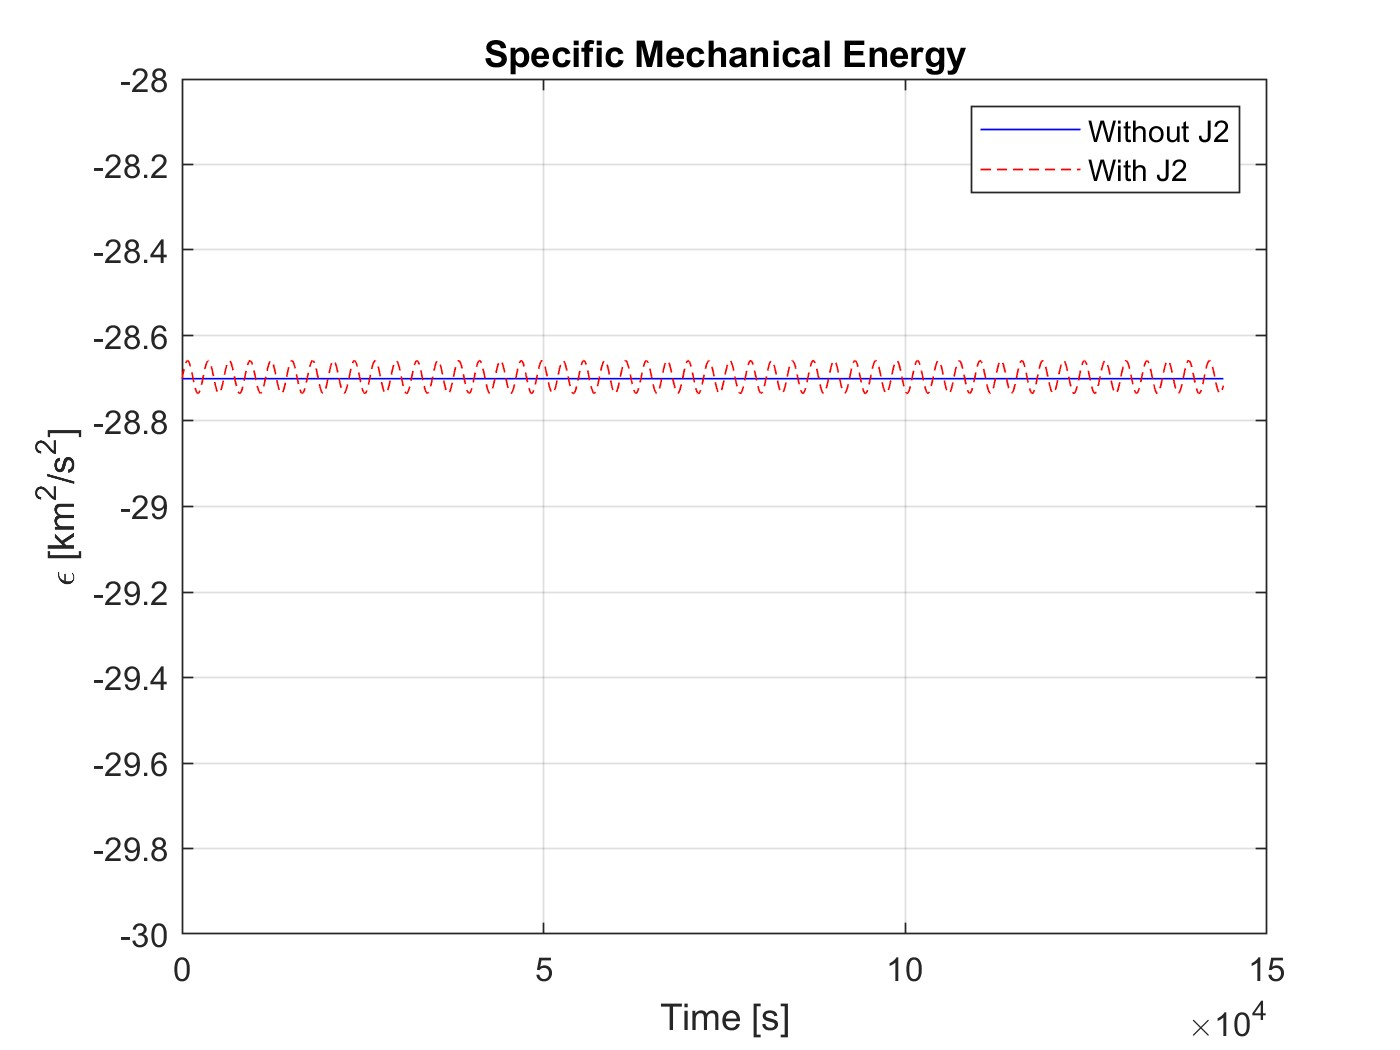
\includegraphics[width=0.5\linewidth]{PS1/Figures/Epsilon_J2_Comparison.jpg}
    \caption{Comparison of Specific Mechanical Energy with and without J2 perturbations over 25 orbits}
    \label{fig:specific_energy}
\end{figure}

\subsubsection{Osculating vs. Mean Orbital Elements with J2 Comparison}\label{sec:osc_mean_J2}
Now, to compare these results with the secular Gauss Variational Equations for J2 with mean orbital elements, we numerically integrate the following linear differential equations:
\begin{align}
\frac{d e_x}{dt} &= -\frac{3}{4} n J_2 \left( \frac{R_\oplus}{a \left(1 - (e_x^2 + e_y^2)\right)} \right)^2 e_y (5 \cos^2 i - 1) \\
\frac{d e_y}{dt} &= \phantom{-}\frac{3}{4} n J_2 \left( \frac{R_\oplus}{a \left(1 - (e_x^2 + e_y^2)\right)} \right)^2 e_x (5 \cos^2 i - 1) \\
\frac{d\Omega}{dt} &= -\frac{3}{2} n J_2 \left( \frac{R_\oplus}{a \left(1 - (e_x^2 + e_y^2)\right)} \right)^2 \cos i  \\
\frac{du}{dt} &= \frac{3}{4} n J_2 \left( \frac{R_\oplus}{a \left(1 - (e_x^2 + e_y^2)\right)} \right)^2 
\left[ \sqrt{1 - (e_x^2 + e_y^2)} (3 \cos^2 i - 1) + (5 \cos^2 i - 1) \right] \quad 
\end{align}

Figure \ref{fig:osc_mean_oe} superimposes the resulting mean and osculating orbital elements on top of each other. As expected, the mean semi-major axis, eccentricity, and inclination remain constant even with J2. For these elements, the osculating elements are purely periodic, agreeing with the mean ones. For RAAN, there both mean and osculating exhibit a clear secular growth. For both argument of periapsis and true anomaly, the osculating elements exhibit periodic and secular behavior. The secular drift in both lines up with the secular drift seen in the mean elements.

\begin{figure}[H]
    \centering
    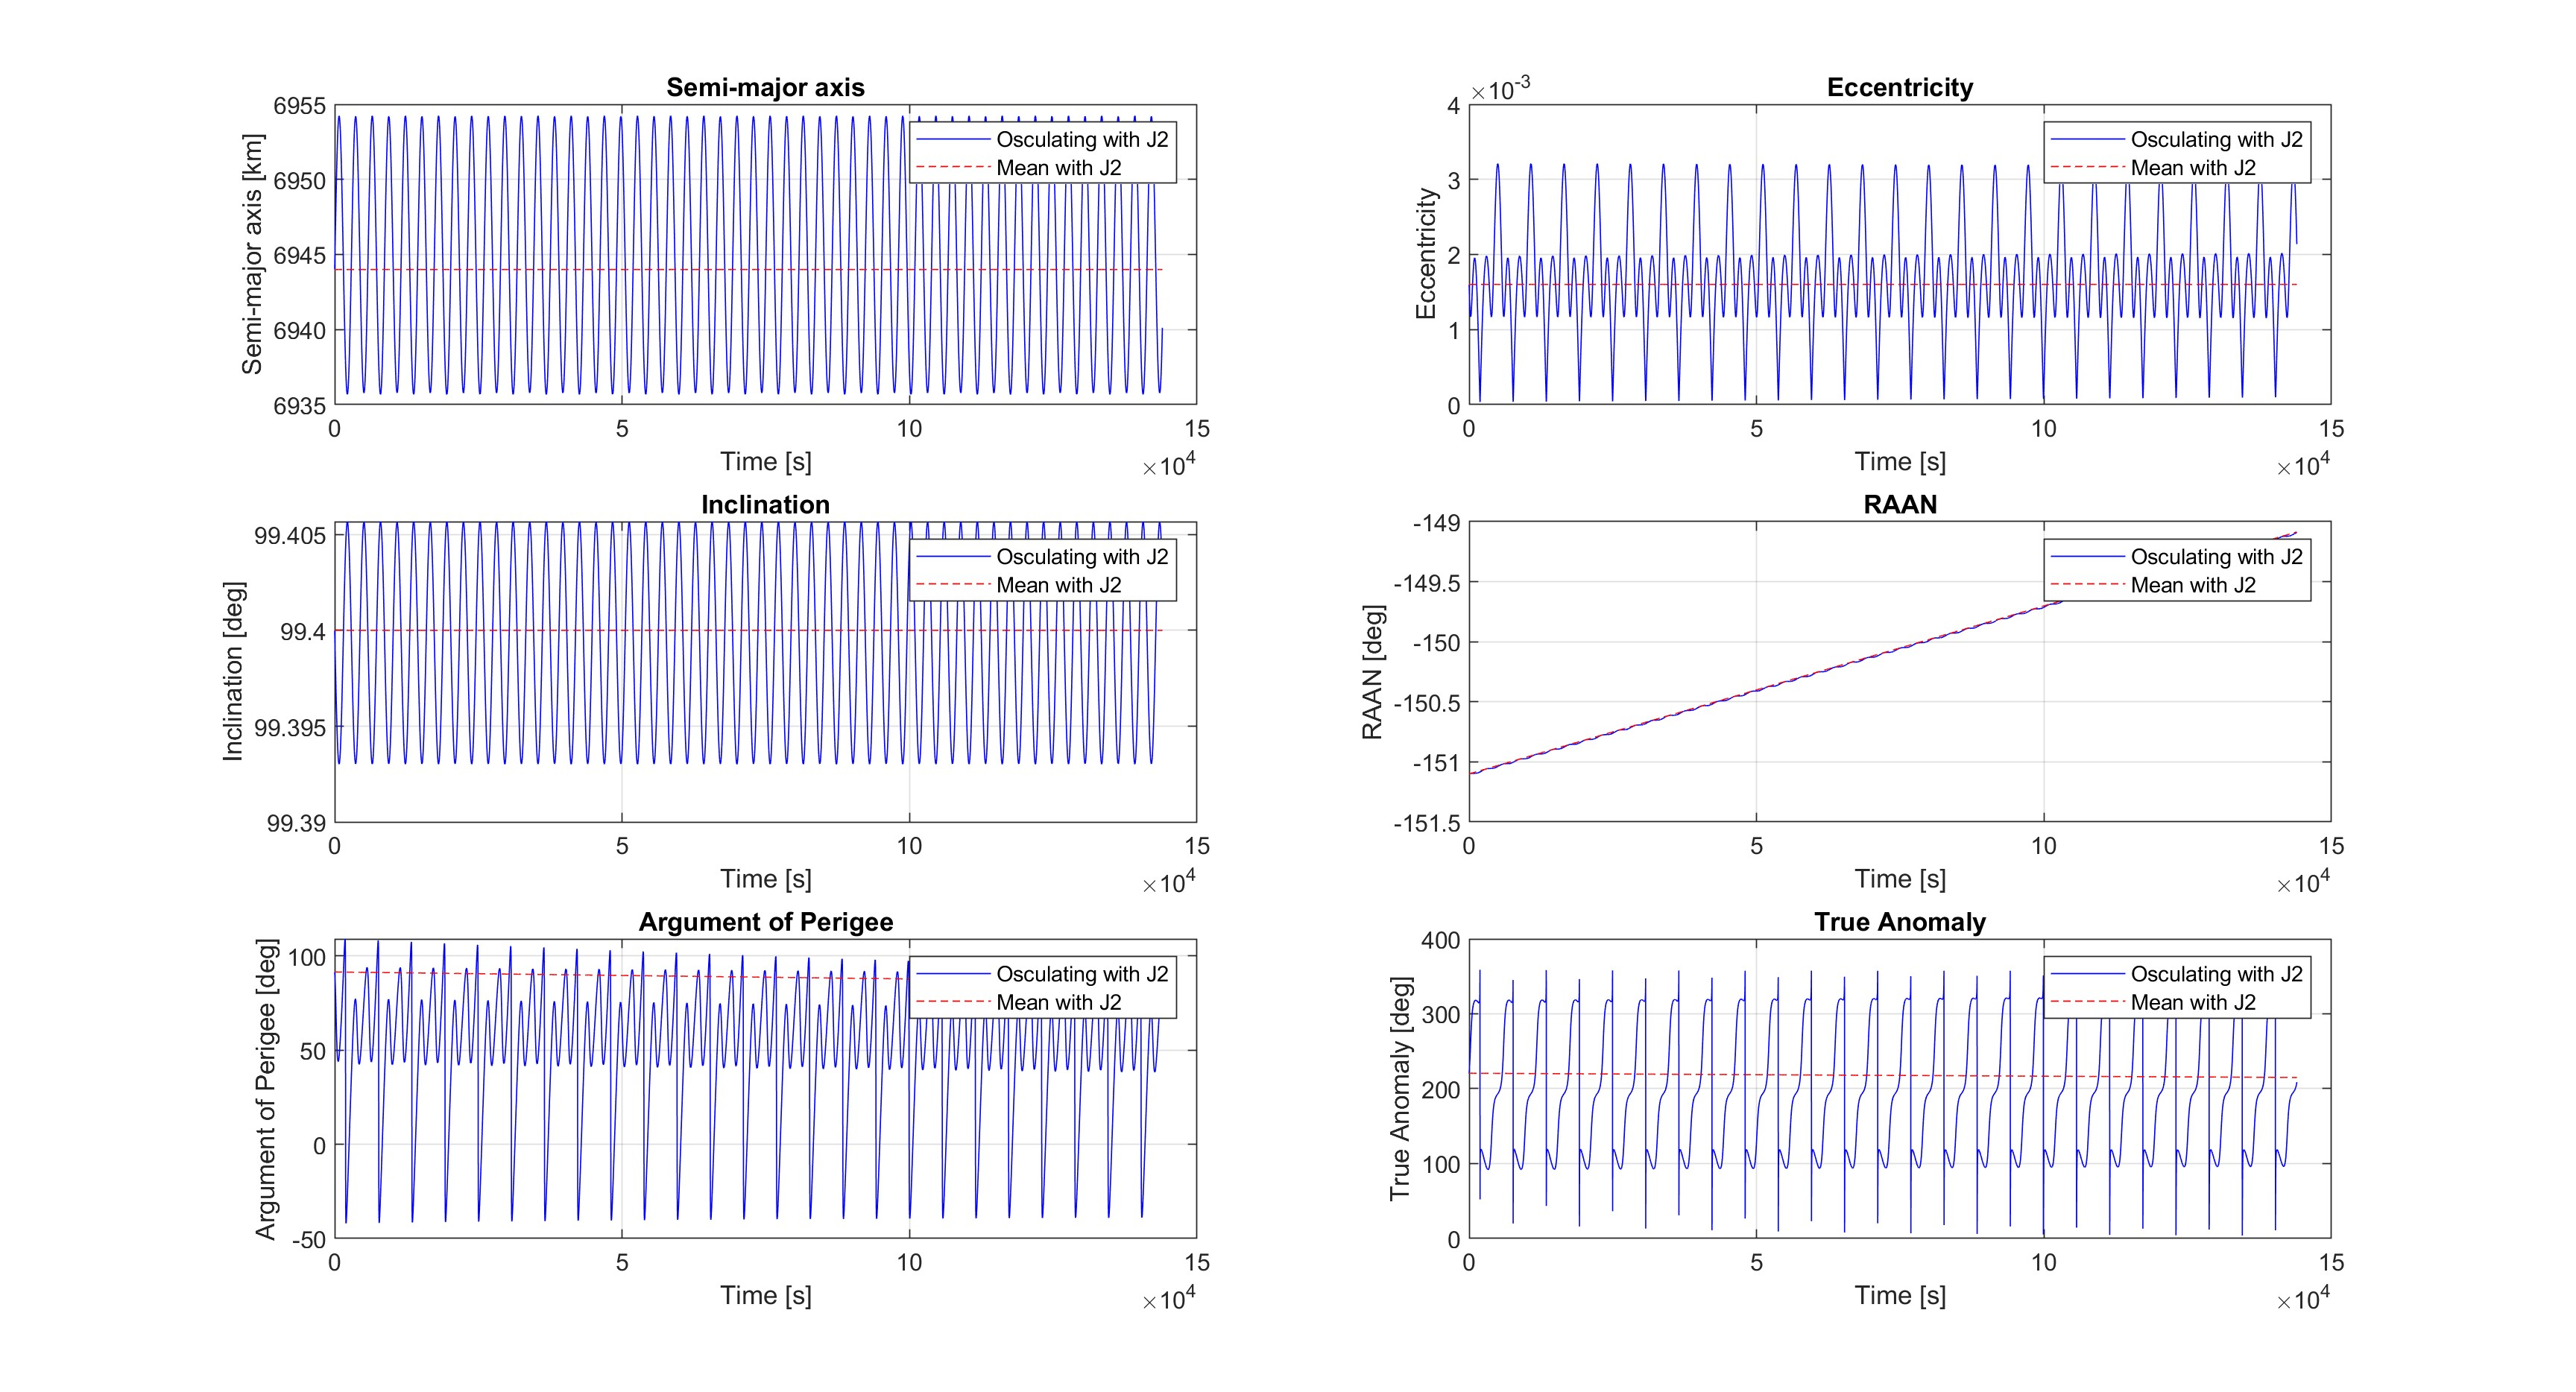
\includegraphics[width=1.1\linewidth]{PS1/Figures/OE_mean_osc_J2_comparison.jpg}
    \caption{Osculating vs Mean Orbital Elements with J2}
    \label{fig:osc_mean_oe}
\end{figure}

\subsubsection{Issues with Comparison}\label{sec:comp_issues}
Issues could arise from the comparison of osculating and mean orbital elements due to the initialization procedure. Specifically, we interpreted our initial orbital elements as osculating at first and then as mean states later on. To ensure that the comparisons remain consistent, it would be most appropriate to convert our initial orbital elements from mean to osculating at first using Brower's Theory. Furthermore, to ensure that both methods align, the final results from osculating could be converted to mean elements to numerically determine if there are any discrepancies, rather than by visual inspection.

\newpage
\section{Problem Set 2}
\subsection{Everything is Relative}

\subsubsection{Variations in Initial Orbital Elements} \label{sec:rel_init_oe}
We will use the initial quasi-nonsingular relative orbital elements (ROE) given in section \ref{sec:ROE_init}, except with zero difference in semi-major axis ($\delta a =0$). Using the chief's initial quasi-nonsingular absolute orbital elements, we can find the initial absolute orbital elements and then the initial position and velocity in ECI of both of the deputy satellites (SV2 and SV3), through the following method: 

The subscript $o$ indicates the chief or "observer", while the subscript $t$ indicates the deputy or "target". First, we convert the chief semi-major axis from km to m to agree with the units of the ROEs:
\begin{align}
   a_o \leftarrow a_o \cdot 10^3 
\end{align}


Then, we compute the deputy semi-major axis, eccentricity components, inclination, RAAN, and argument of latitude using the ROEs from Starling:
    \begin{align}
    a_t &= \frac{a_o + d_a}{10^3} \\
    e_{x,t} &= \frac{d_{e_x}}{a_o} + e_{x,o} \\
    e_{y,t} &= \frac{d_{e_y}}{a_o} + e_{y,o} \\
    i_t &= \frac{d_{i_x}}{a_o}  + i_o \\
    \Omega_t &= \frac{d_{i_y}}{a_o \cdot \sin(i_o)}  + \Omega_o \\
    u_t &=  \frac{d_\lambda}{a_o}+ u_o - (\Omega_t - \Omega_o) \cdot \cos(i_o)
\end{align}


Then the quasi-nonsingular orbital elements can be converted to the Keplerian orbital elements through the method outlined in section \ref{sec:initial_oe}. Finally, the Keplerian orbital elements can be converted to position and velocity in the ECI frame through the method outlined in section \ref{sec:initial_ECI}. This results in the initial ECI position and velocity of both the deputies: 

\begin{align}
    \mathbf{r}_{\text{SV2}} &=
    \begin{bmatrix}
    -3574.8655 \\
    -2953.8783 \\
    -5180.4446
    \end{bmatrix} \text{km} \\
    \mathbf{v}_{\text{SV2}} &=
    \begin{bmatrix}
    -5.3901 \\
    -2.0500 \\
    \phantom{-}4.8991
    \end{bmatrix} \text{km/s} \\
    \mathbf{r}_{\text{SV3}} &=
    \begin{bmatrix}
    -3606.2292 \\
    -2965.3946 \\
    -5150.6778
    \end{bmatrix} \text{km} \\
    \mathbf{v}_{\text{SV3}} &=
    \begin{bmatrix}
    -5.3652 \\
    -2.0292 \\
    \phantom{-}4.9357
    \end{bmatrix} \text{km/s}
\end{align}

\subsubsection{Numerical Integration of Non-linear Equations for Relative Motion} \label{sec:nonlinear_rel_eom}
Given the initial ECI conditions of the chief (SV1) and the deputies (SV2 and SV3), we can find the initial position and velocity of the deputies in the RTN frame of the chief. The rotation matrix from ECI to RTN is the same as in Equations \ref{eq:eci2rtn} to \ref{eq:v_rtn}. 

We take $\boldsymbol{\rho}$ as the relative position between the chief and deputy (for the equations below, we use SV2), so $\boldsymbol{\rho}^{RTN}$ is relative position of the deputy in the chief's RTN frame. Similarly, $\boldsymbol{\dot{\rho}}^{RTN}$ is the relative velocity of the deputy in the chief's RTN frame.

\begin{align}
    \boldsymbol{\rho}_{SV2}^{ECI} &= \boldsymbol{r}^{ECI}_{SV2} - \boldsymbol{r}^{ECI}_{SV1}\\
    \boldsymbol{\rho}^{RTN}_{SV2} &= Q_{eci2rtn} \boldsymbol{\rho}_{SV2}^{ECI} \\
    \boldsymbol{\dot{\rho}}^{RTN}_{SV2} &= Q_{eci2rtn} \left(\boldsymbol{v}^{ECI}_{SV2} - \boldsymbol{v}^{ECI}_{SV1}\right)  - \omega_{RTN} \times \boldsymbol{\rho}^{RTN}_{SV2} \label{eq:v_rtn_rel}
\end{align}

where $\omega_{RTN} = \begin{bmatrix}
    0 & 0 & ||r\times v ||/||r||^2
\end{bmatrix}$. We can define $\boldsymbol{\rho}^{RTN}$ and $\boldsymbol{\dot{\rho}}^{RTN}$ (Here, the time derivative accounts for the rotating RTN frame) to be

\begin{align}
    \boldsymbol{\rho}^{RTN} &= \begin{bmatrix}
        x & y & z
    \end{bmatrix}^T, \\
    \boldsymbol{\dot{\rho}}^{RTN} &= \begin{bmatrix}
        \dot{x} & \dot{y} & \dot{z}
    \end{bmatrix}^T 
\end{align}

The non-linear equations of motion for relative motion give us a method to numerically propagate $x, y, \text{and} \ z$. The equations of motion are given by

\begin{align}
\ddot{x} &= 2\dot{\theta}_0 \dot{y} + \ddot{\theta}_0 y - \dot{\theta}_0^2 x -\frac{\mu (r_0 + x)}{\left[(r_0 + x)^2 + y^2 + z^2\right]^{3/2}} + \frac{\mu}{r_0^2} \\
\ddot{y} &= - 2\dot{\theta}_0 \dot{x} - \ddot{\theta}_0 x + \dot{\theta}_0^2 y  -\frac{\mu y}{\left[(r_0 + x)^2 + y^2 + z^2\right]^{3/2}} \\
\ddot{z} &= -\frac{\mu z}{\left[(r_0 + x)^2 + y^2 + z^2\right]^{3/2}}
\end{align}

The value $r_0$ is the radial position of the chief when expressed in the RTN frame (or, the norm of the position vector of the chief) $\boldsymbol{r}_0 = ||\boldsymbol{r}^{ECI}_{SV1}|| = \boldsymbol{r}^{RTN}_{SV1, x}$ 
Here, $\dot{\theta}$ is the angular velocity of the chief (and thus the angular velocity of the RTN frame), and $\ddot{\theta}$ is the angular acceleration of the chief. We can get 
\begin{align}
    \dot{\theta} &= \frac{{||\boldsymbol{r}_{SV1}^{ECI} \times \boldsymbol{v}_{SV1}^{ECI}||}}{r_0^2} \\
    \ddot{\theta} &= -\frac{2\dot{r}_0\dot{\theta}}{r_0}
\end{align}

Here, $\dot{r}_0$ is the rate of change in the length of the position vector of the chief. A convenient way to get this is to take the radial component of the chief's velocity in its RTN frame.

\begin{align}
    \dot{r}_0 = \boldsymbol{v}^{RTN}_{SV2, x}
\end{align}

With these differential equations and the initial conditions in RTN, the relative motion of the deputy satellites is propagated using RK4 (Runga-Kutta-4) through the entire duration that the chief is propagated. The specifications of the time-steps are the same as Equation \ref{eq:timestep}.

All the above operations are also repeated for the third satellite, SV3/Docker, for which the initial conditions are given in Section \ref{sec:rel_init_oe}.
The results of the propagation are shown in Figures \ref{fig:rel_3d_traj}, \ref{fig:rel_3d_proj}, \ref{fig:rel_pos_vel_rtn_sv2}, and \ref{fig:rel_pos_vel_rtn_sv3}.

\subsubsection{Computing Relative Orbits using FODE of Absolute Motion}\label{sec:rel_FODE_num_int}

In this method, we perform the absolute orbit propagation of the three satellites SV1, SV2, and SV3 using just the fundamental orbital differential equations of absolute motion utilized in Section \ref{sec:fode_simulation}. Once the motion of all three satellites is calculated, the positions and velocities of the deputies SV2 and SV3 can be converted into the RTN frame of the chief using the procedure described in Section \ref{sec:nonlinear_rel_eom} in equations \ref{eq:q_eci2rtn_rel} to \ref{eq:v_rtn_rel}. This FODE propagation is done with the same numerical method (RK4) and time-steps as the nonlinear relative motion method, given in equation \ref{eq:timestep}. The results of this method are shown and compared in Figures \ref{fig:rel_3d_traj}, \ref{fig:rel_3d_proj}, \ref{fig:rel_pos_vel_rtn_sv2}, and \ref{fig:rel_pos_vel_rtn_sv3}.

It is interesting to note that in Figure \ref{fig:rel_3d_traj}, the relative orbits are not centered around the $x = 0$ point. Instead, the deputy satellites always have a negative radial position despite having the same semi-major axis as the chief. This is because we are using rectilinear co-ordinates instead of curvi-linear co-ordinates, and so these plots don't correct for the curvature of the earth, which is non-negligible when one has large cross-track separations.

\begin{figure}[H]
    \centering
    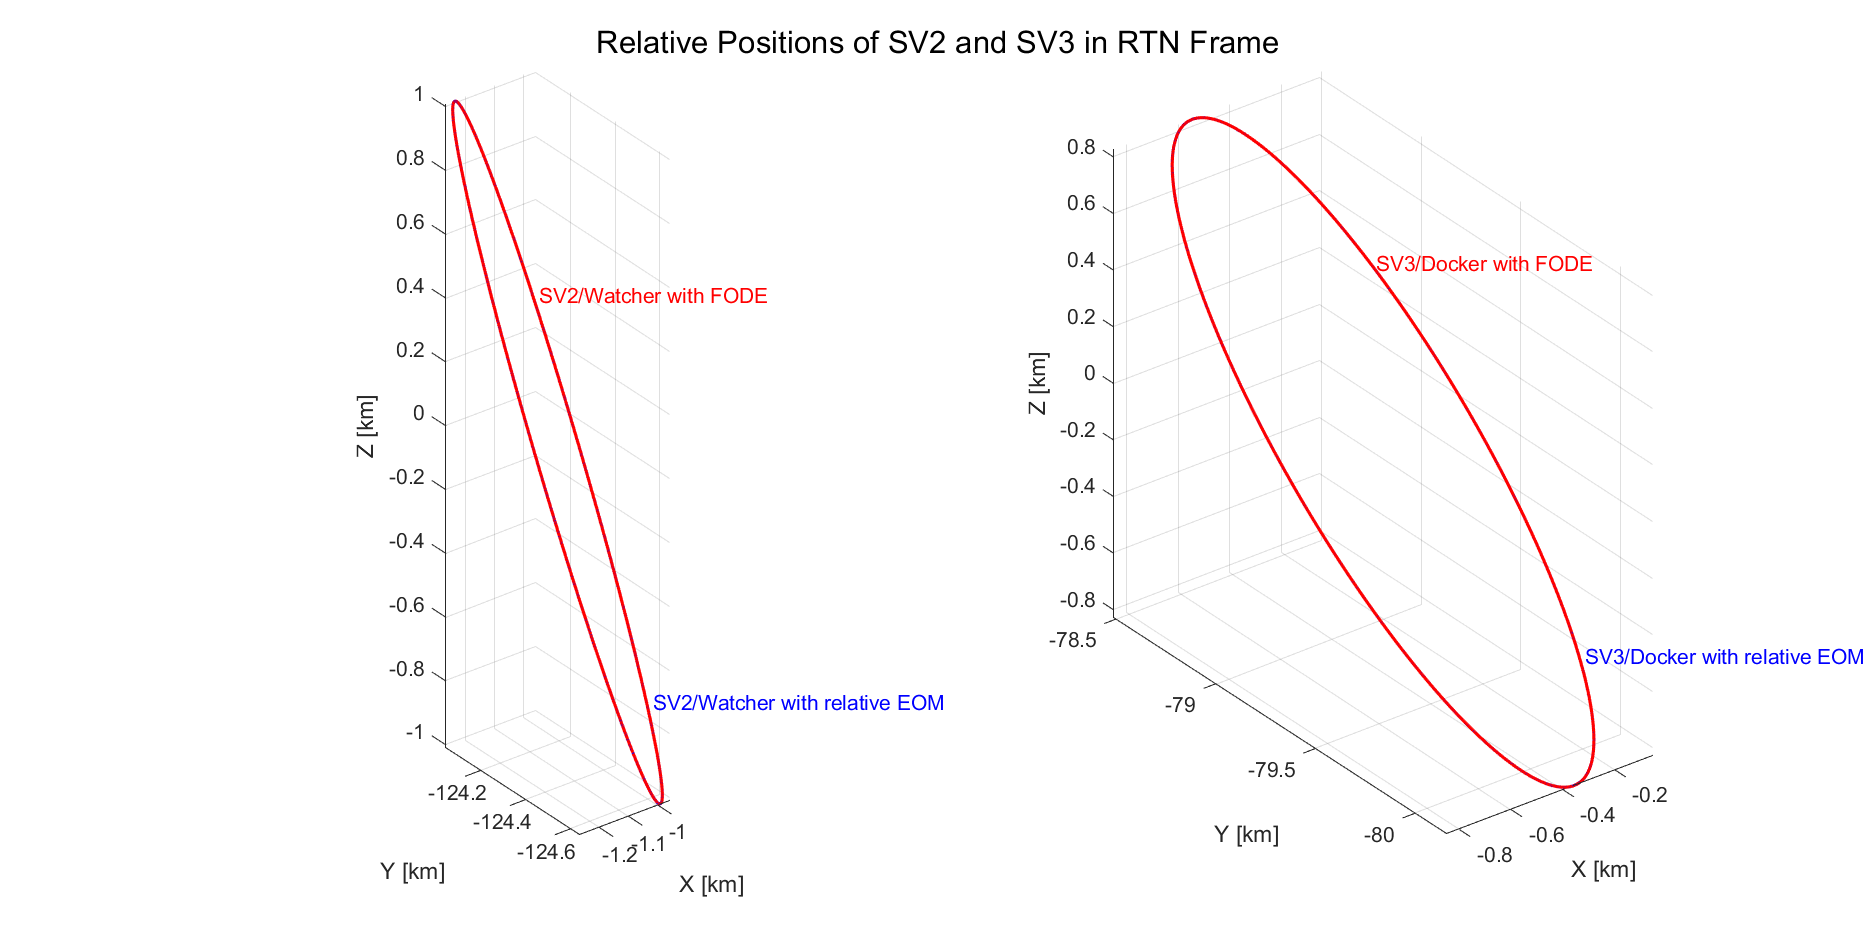
\includegraphics[width=0.9\linewidth]{sim/figures/SV2_SV3_3d_traj_rel.png}
    \caption{The 3D trajectories of SV2 and SV3 with the relative orbit propagation and FODE absolute motion propagation}
    \label{fig:rel_3d_traj}
\end{figure}

\begin{figure}[H]
    \centering
    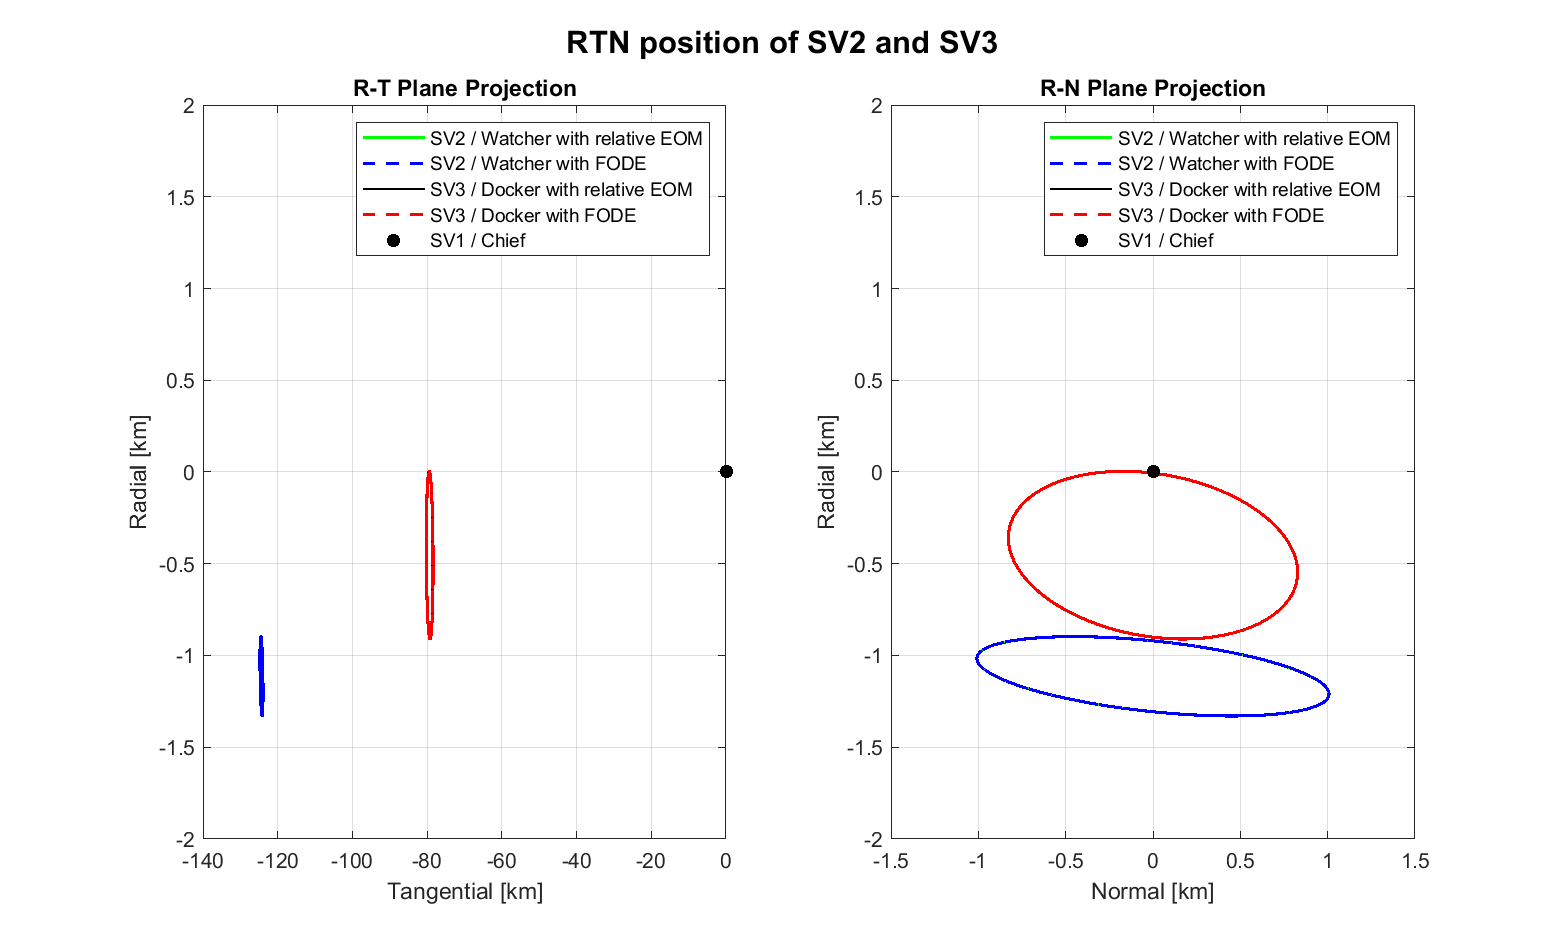
\includegraphics[width=0.9\linewidth]{sim/figures/RTN_projection.png}
    \caption{Projection of the trajectory to the Radial-Tangential and Radial-Normal planes, for both SV2 and SV3, and for both methods.}
    \label{fig:rel_3d_proj}
\end{figure}

\begin{figure}[H]
    \centering
    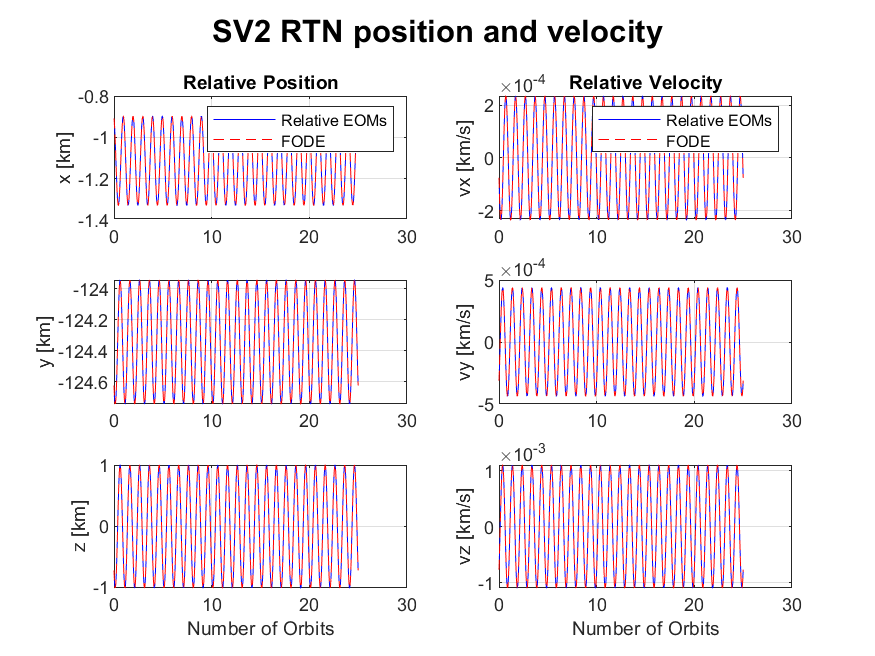
\includegraphics[width=0.7\linewidth]{sim/figures/SV2_rel_pos_vel.png}
    \caption{The RTN position and velocity of SV2, for both methods of relative orbit calculation.}
    \label{fig:rel_pos_vel_rtn_sv2}
\end{figure}

\begin{figure}[H]
    \centering
    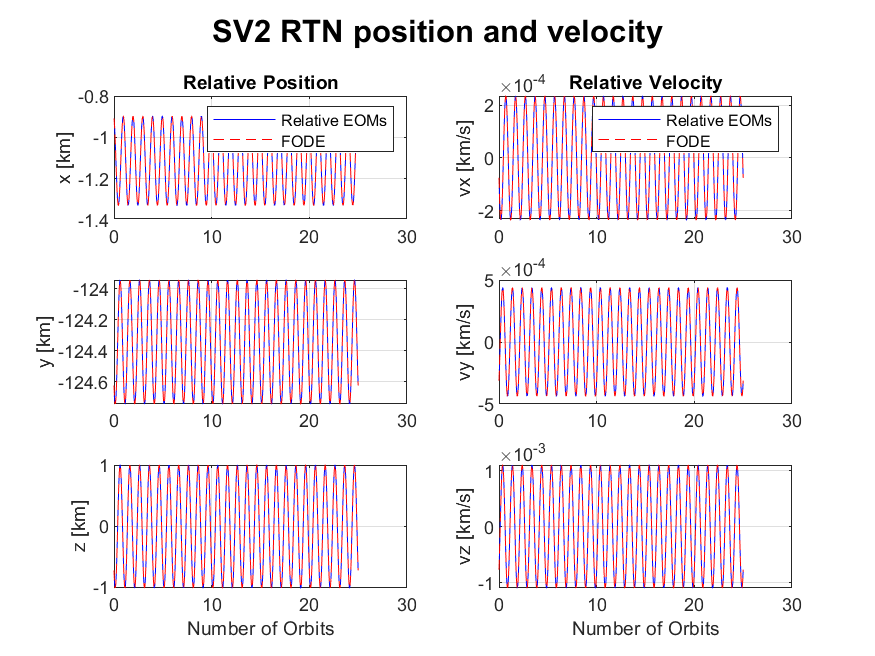
\includegraphics[width=0.7\linewidth]{sim/figures/SV2_rel_pos_vel.png}
    \caption{The RTN position and velocity of SV3, for both methods of relative orbit calculation.}
    \label{fig:rel_pos_vel_rtn_sv3}
\end{figure}

\subsubsection{Comparison of Relative Orbit Calculation Methods}
Since the two methods used above for relative orbit calculation are mathematically equivalent irrespective of initial conditions utilized, the only difference in the results should be numerical errors. Figures \ref{fig:error_in_SV2_rel} and \ref{fig:error_in_SV3_rel} showcase the error between the two methods for SV2 and SV3 respectively.

\begin{figure}
    \centering
    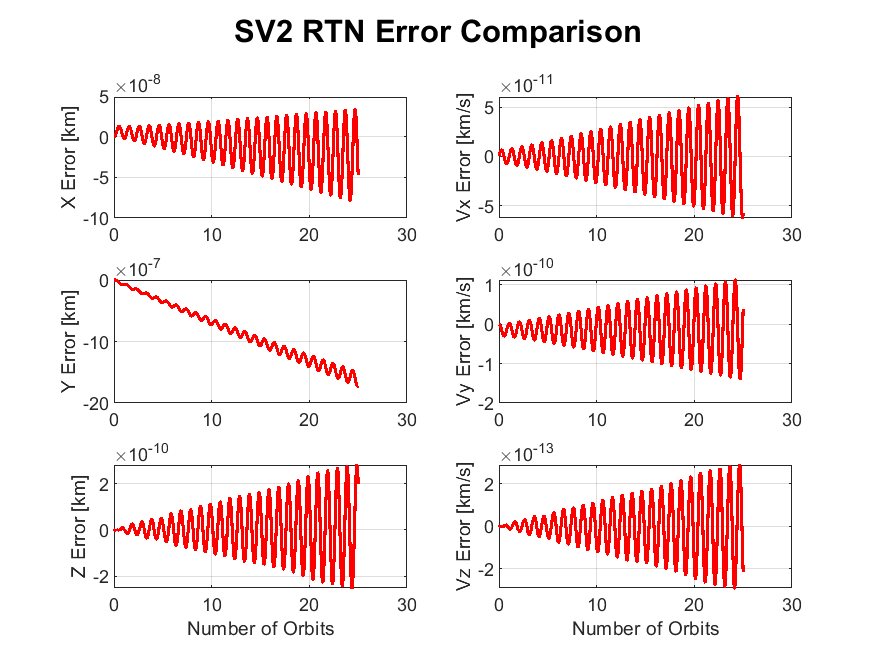
\includegraphics[width=0.75\linewidth]{sim/figures/SV2_error_in_rel_methods.png}
    \caption{Error between the relative orbits of SV2 calculated by FODE methods and Nonlinear relative EOM methods.}
    \label{fig:error_in_SV2_rel}
\end{figure}

\begin{figure}
    \centering
    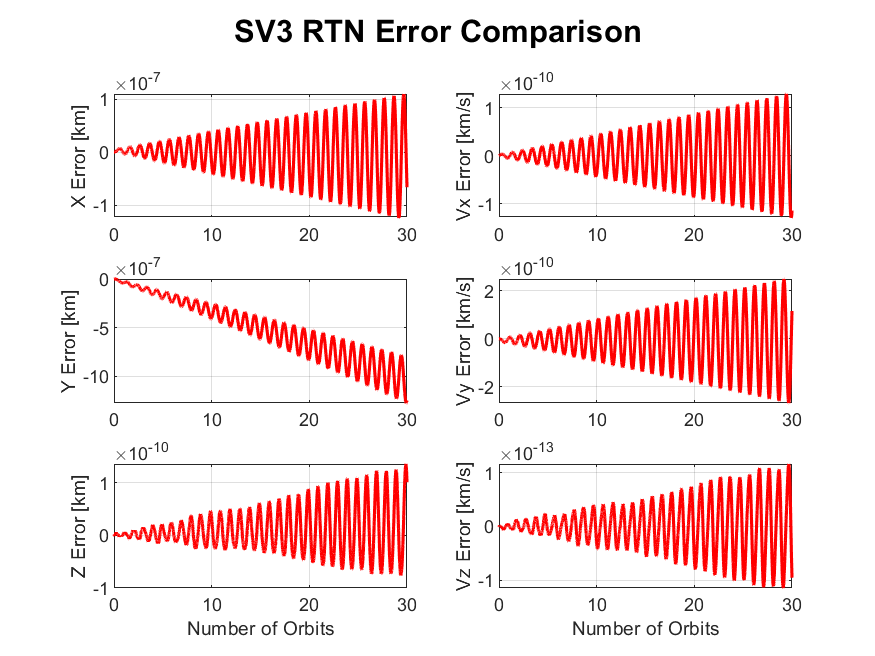
\includegraphics[width=0.75\linewidth]{sim/figures/SV3_error_in_rel_methods.png}
    \caption{Error between the relative orbits of SV3 calculated by FODE methods and Nonlinear relative EOM methods.}
    \label{fig:error_in_SV3_rel}
\end{figure}

We see that using fine time-steps of 11.5 seconds, we can keep the numerical error between the two methods contained to negligible amounts.

This also holds when the initial condition has a semi-major axis difference, which we can see in Figure \ref{fig:error_in_SV2_rel_nonzero_a} for SV2 when its initial conditions of SV2 have a non-zero difference in the semi-major axis. Although the error has a different profile than in the previous plots, the error is still at a much smaller magnitude than the actual values, so is negligible, and can be attributed to numerical error. The different error profile is due to the drift in the RTN frame due to the difference in semi-major axis. 

\begin{figure}
    \centering
    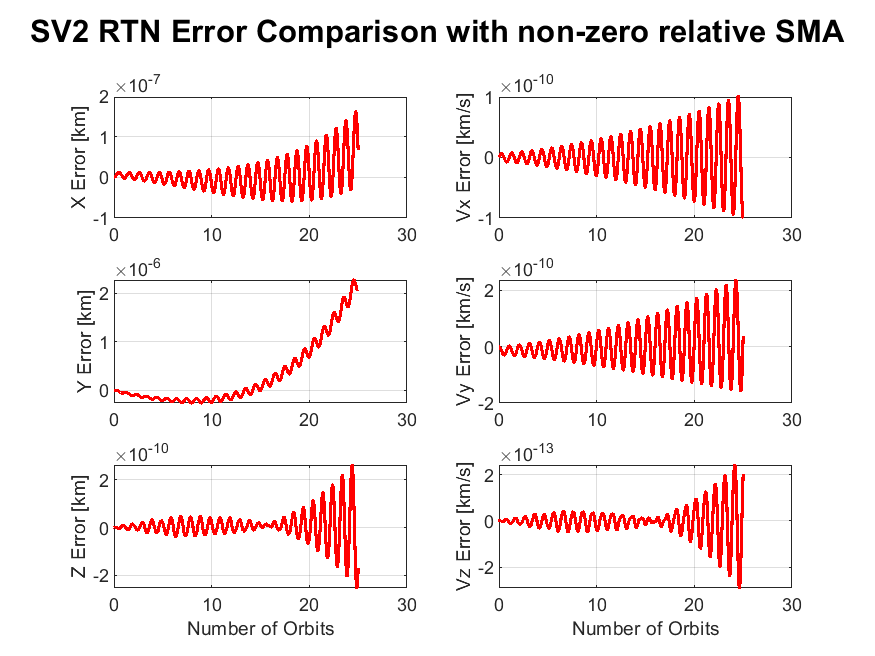
\includegraphics[width=0.7\linewidth]{sim/figures/SV2_error_in_rel_methods_nonzero_a.png}
    \caption{Error between the relative orbits of SV2 calculated by FODE methods and Nonlinear relative EOM methods, in a case where there is a relative semi-major axis difference.}
    \label{fig:error_in_SV2_rel_nonzero_a}
\end{figure}

\subsubsection{Derivation of Impulsive Maneuver for Bounded Period Motion}
To re-establish a bounded periodic relative motion between the deputy and the chief, the specific mechanical energies and, thus, the semi-major axes of the orbits must match. For a circular chief orbit (or near-circular as in our case), an equilibrium continuum exists that satisfies the energy matching condition: when the deputy is co-located on the same circular orbit of the chief. To achieve this condition, the semi-major axis of the deputy must be the same as the chief's, leading to both having the same mean motion. Therefore, an impulsive maneuver to adjust the deputy's semi-major axis is chosen. The Gauss Variational Equation (GVE) for semi-major axis is given as follows:
\begin{align}
\frac{da}{dt} &= \frac{2e \sin f}{n \sqrt{1 - e^2}} f_r + \frac{2a \sqrt{1 - e^2}}{n r} f_t
\end{align}
In order to find the size (delta-v) and location of the maneuver, we can integrate the GVE over an impulsive maneuver delta-v with constant orbit elements, using the following framework:
\begin{align}
\int_{t^-}^{t^+} \frac{d\vec{o}}{dt} dt &= \int_{t^-}^{t^+} \frac{\partial \vec{o}}{\partial \vec{v}} \left( \vec{a} \right) dt
\end{align}
Applying this to the semi-major axis GVE results in the following:
\begin{align}
\Delta a = \int \frac{da}{dt} dt = \int \left( \frac{2a \sqrt{1 - e^2}}{n r} \cdot f_t \right) dt
\end{align}
And then assuming impulsive maneuver, \( \int f_t dt = \Delta v_t \):
\begin{align}
\Delta a = \frac{2a \sqrt{1 - e^2}}{n r} \Delta v_t
\end{align}
Rearranging for $\Delta v_t$:
\begin{align}
\Delta v_t = \frac{n r}{2a \sqrt{1 - e^2}} \Delta a
\end{align}
This can be simplified for near-circular orbits \( e = 0, a \approx r \), however we will use the more accurate previous expresision:
\begin{align}
\Delta v_t = \frac{n}{2} \Delta a
\end{align}

Note that we ignore the radial component of the GVE because radial acceleration is not as efficient at changing \( a \) as tangential acceleration is. Also, the radial term only contributes if \( e \neq 0 \), and the maneuver does not occur at periapsis or apoapsis due to its dependence on true anomaly \(\sin f\). While there is some eccentricity, the second condition will not hold for our maneuver. Thus, the most fuel-efficient maneuver will be in the along-track direction.

For the most fuel-efficient location, the impulsive maneuver should be applied at periapsis due to the Oberth effect. Note that this is assuming the relative phasing of the deputy from the chief is less important than fuel efficiency. Also note that if the orbit is near-circular, there is not much added efficiency by performing at the periapsis as compared to anywhere else due to very small velocity changes throughout the orbit.

Therefore, the most fuel-efficient impulsive maneuver will be performed at the periapsis of the deputy's orbit in the along-track direction with size $\Delta v_t$. A single-burn maneuver will lead to a change in the eccentricity, which is acceptable for our purposes in this case. If no eccentricity change was desired, this could be accomplished with splitting up the single maneuver into two burns with one at the periapsis and one at the apoapsis, each with half of the original delta-v. 

\subsubsection{Application of Impulsive Maneuver for Bounded Period Motion}
To apply the impulsive maneuver to re-establish bounded periodic motion, we first found the required $\Delta v_t$ from the desired $\Delta a$ to match the chief's semi-major axis. The differences in semi-major axes of the deputies were arbitrarily set to be large to create a noticeable drift. Specifically, the initial conditions were:

\begin{align*}
\delta a_{\text{SV2, init}} &= 200 \text{ m} \\
\delta a_{\text{SV3, init}}  &= -1000 \text{ m}
\end{align*}

Both orbits were propagated for approximately 12 orbits. Then burn was performed at the periapsis of the 12th orbit for fuel-optimality. As seen in both Figure \ref{fig:SV2_rel_pos_vel_eom_maneuver} and \ref{fig:SV3_rel_pos_vel_eom_maneuver}, the drift in radial ($x$) and tangential ($y$) positions was stopped by the maneuver. Instead of oscillations with secular drift, there are now purely oscillations post-maneuver. The secular drift arises from differences in the mean motions of the deputy and chief due to the difference in semi-major axis of the two. The drift cancellation arises from the equilibrium condition of semi-major axis matching. The amplitude of oscillations is related to the phasing of the deputies with respect to the chief, which is a function of timing and relative positioning during the maneuver. Note that while the changes in relative position appear to be instantaneous, they occur over a short period of time. The magnitude of these changes arises from the arbitrary initial conditions set and the amount of drift before the maneuver is applied. 

\begin{figure}[H]
    \centering
    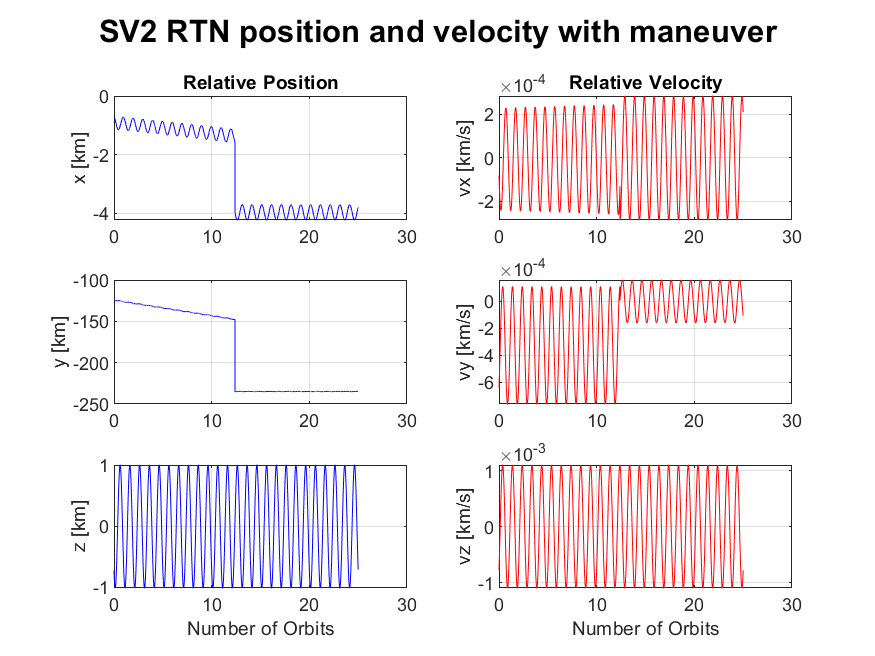
\includegraphics[width=0.7\linewidth]{sim/figures/SV2_rel_pos_vel_eom_maneuver.png}
    \caption{SV2 RTN position and velocity with maneuver applied}
    \label{fig:SV2_rel_pos_vel_eom_maneuver}
\end{figure}

\begin{figure}[H]
    \centering
    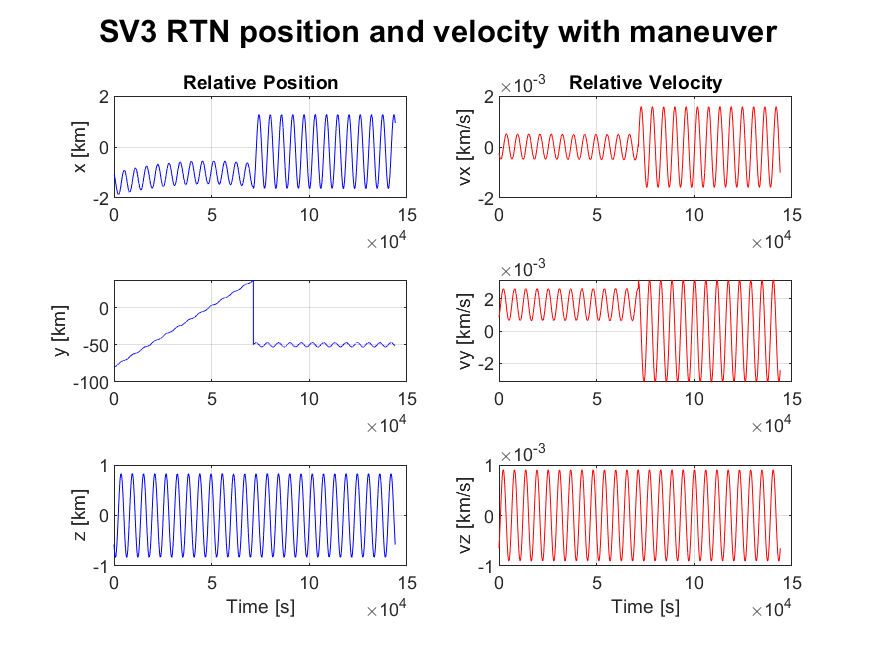
\includegraphics[width=0.7\linewidth]{sim/figures/SV3_rel_pos_vel_eom_maneuver.png}
    \caption{SV3 RTN position and velocity with maneuver applied}
    \label{fig:SV3_rel_pos_vel_eom_maneuver}
\end{figure}
\newpage
\section{Problem Set 3}
\subsection{We are Close in Near-Circular Orbits}

\subsubsection{Initial Conditions for HCW}

We would like to use the Hill-Clohessy-Wiltshire (HCW) equations to give us a clear solution to the relative motion of the deputy satellites. However, the HCW equations assume that the motion of the depity with respect to the chief is very small compared to the orbit radius, as they rely on linearizing the non-linear equations of motion the The initial conditions for this are built over the original absolute and relative initial conditions for SV1, SV2, and SV3 that were previous defined in Table \ref{tab:abs_oe} and Table \ref{tab:relative_oe}.

The eccentricity of SV1 is already very low, as seen in Table \ref{tab:abs_oe_kepler} (and meets the conditions for applying HCW). Therefore, the orbital elements of the chief did not need to be modified. However, the relative orbital elements initial conditions create a large separation between SV1 and SV2/SV3. So the quasi-nonlinear relative orbital elements are modified to be as in Table \ref{tab:relative_oe_hcw} below. These are written in order as described in Equation \ref{eq:quasi_nonsign_roe}.

\begin{table}[h!]
\centering
\begin{tabular}{ll}
\toprule
\textbf{ID} & \textbf{HCW Conditions} \\
\midrule
SV2 & $\delta\boldsymbol{\alpha} = [0, 0, 0, 100, 0, 1000]~\text{m}$ \\
SV3 & $\delta\boldsymbol{\alpha} = [0, 0, 0, 200, 0, 800]~\text{m}$ \\
\bottomrule
\end{tabular}
\caption{Quasi-Nonsingular Relative Orbit Parameters for SV2 and Sv3 to apply for HCW}
\label{tab:relative_oe_hcw}
\end{table}

The main differences in these quasi-nonsingular relative orbital elements (and the justification for these changes), are:
\begin{itemize}
    \item $\delta\alpha$ is 0 for both SV2 and SV3, so that they have the same semi-major axes as SV1.
    \item The $\delta\lambda$ for both deputy satellites is reduced to 0. This helps reduce the separation between the deputies and the chief
    \item $\delta e_x$and $\delta i_x$ are set to zero for convenience, and to easily create a $\boldsymbol{e}-\boldsymbol{i}$ vector angle separation of $0^\circ$.
    \item $\delta e_y$ and $\delta i_y$ are set to convenient values close to the original relative orbital elements in Table \ref{tab:relative_oe}.
\end{itemize}

Based on these initial conditions, we see that the ratio of the maximum separation between spacecraft is small relative to the distance of the chief from the primary attractor.

TODO: Add something here to show this.

\subsubsection{Transforming the Initial Conditions} \label{sec:hcw_initial_conditions}
We can convert the initial conditions set in Table \ref{tab:relative_oe_hcw} to different representations. The initial conditions for the chief are not recalculated, as these have not been modified from previous sections.

\textbf{ECI and Absolute Orbital Elements} \\
Using the transformations highlighted in Equation \label{eq:quasi_nonsign_roe}, 
we convert the quasi-nonsingular relative orbital elements into absolute orbital elements. The results for SV2 and SV3 are given in Table \ref{tab:abs_oe_kepler_SV2_HCW} and Table \ref{tab:abs_oe_kepler_SV3_HCW}. The absolute orbital elements of the chief remain the same as in Table \ref{tab:abs_oe_kepler}.

TODO: Need to update these tables.

\begin{table}[h]
\centering
\begin{tabular}{cccccc} \hline
    $a$ & $e$ & $i$ & $\omega$ & $\Omega$ & $\nu$ \\ \hline 
     6944 km & 0.0016 & 99.4 $^\circ$ & 91.432$^\circ$ & -151.1$^\circ$ & -139.45$^\circ$ \\ \hline
\end{tabular}
\caption{Initial Keplerian Orbit Parameters of SV2, modified for applying HCW}
\label{tab:abs_oe_kepler_SV2_HCW}
\end{table}

\begin{table}[h]
\centering
\begin{tabular}{cccccc} \hline
    $a$ & $e$ & $i$ & $\omega$ & $\Omega$ & $\nu$ \\ \hline 
     6944 km & 0.0016 & 99.4 $^\circ$ & 91.432$^\circ$ & -151.1$^\circ$ & -139.45$^\circ$ \\ \hline
\end{tabular}
\caption{Initial Keplerian Orbit Parameters of SV3, modified for applying HCW}
\label{tab:abs_oe_kepler_SV3_HCW}
\end{table}

These Keplerian orbital elements are then converted to ECI co-ordinates using the expressions provided in Section \ref{sec:initial_ECI}. The initial ECI co-ordinates of the chief remain the same as in Equation \ref{eq:SV1_initial_ECI}. Equations \ref{eq:SV2_HCW1_ECI_initial} and \ref{eq:SV3_HCW1_ECI_initial} provide the ECI co-ordinates of SV2 and SV3. 


\begin{align} \label{eq:SV2_HCW1_ECI_initial}
    r_{0, ECI, SV2} &= \begin{bmatrix}
        -3091.3 \\
        -2937.0 \\
        -6503.8
    \end{bmatrix} km \\
    v_{0, ECI, SV2} &= \begin{bmatrix}
        -5.0008 \\
        -2.0031 \\
        4.0106
    \end{bmatrix} \frac{km}{s}
\end{align}


\begin{align} \label{eq:SV3_HCW1_ECI_initial}
    r_{0, ECI. SV3} &= \begin{bmatrix}
        -3091.4 \\
        -2937.0 \\
        -6503.7
    \end{bmatrix} km \\
    v_{0, ECI, SV3} &= \begin{bmatrix}
        -5.0009 \\
        -2.0029 \\
        4.0107
    \end{bmatrix} \frac{km}{s}
\end{align}


\textbf{Relative Position and Velocity in Chief's RTN frame, Orbital Element Differences} \\

Since the initial conditions of SV1, SV2, and SV3 are known, we can find the positions and velocities of SV2 and SV3 in SV1's RTN frame using the equations highlighted in Section \ref{sec:nonlinear_rel_eom}. These are provided below in Equations \ref{eq:SV2_HCW_RTN_init} and \ref{eq:SV3_HCW_RTN_init}.

\begin{align} \label{eq:SV2_HCW_RTN_init}
    r_{0, RTN. SV2} &= \begin{bmatrix}
        0.3256 \\
        -0.4989 \\
        -0.5971
    \end{bmatrix} km \\
    v_{0, RTN, SV2} &= \begin{bmatrix}
        -2.0102 \\
        -5.8056 \\
        -7.7372
    \end{bmatrix}\cdot 10^{-4} \frac{km}{s}
\end{align}

\begin{align} \label{eq:SV3_HCW_RTN_init}
    r_{0, RTN. SV2} &= \begin{bmatrix}
        0.2433 \\
        -0.3730 \\
        -0.4914
    \end{bmatrix} km \\
    v_{0, RTN, SV2} &= \begin{bmatrix}
        -1.5210 \\
        -4.3352 \\
        -6.3669
    \end{bmatrix}\cdot 10^{-4} \frac{km}{s}
\end{align}

The differences in the initial orbital elements between the chief and the deputies is best conveyed by the quasi-nonsingular relative orbital elements that are provided in Table \ref{tab:relative_oe_hcw}.

\subsubsection{Computing the Integration Constants}

The Hill-Clohessy Wiltshire equations for linearized relative orbital dynamics allows for analytical solutions of the RTN position $[x, y, z]^\top$ and the RTN velocity $[\dot{x}, \dot{y}, \dot{z}]^\top$ of the deputy satellites in the chief's RTN frame. This solution can be expressed as a function of time, when six integration constants are known (one for each state). The integration constants and the satellite's RTN state are related the Matrix-Vector solution for HCW, given in Equation \ref{eq:HCW_solution}, 


\begin{align} \label{eq:HCW_solution}
\begin{bmatrix}
x \\ y \\ z \\ \dot{x} \\ \dot{y} \\ \dot{z}
\end{bmatrix}
&=
\begin{bmatrix}
a I_{3 \times 3} & 0_{3 \times 3} \\
0_{3 \times 3} & a n I_{3 \times 3}
\end{bmatrix}
\begin{bmatrix}
1 & \sin nt & \cos nt & 0 & 0 & 0 \\
-\frac{3}{2}nt & 2 \cos nt & -2 \sin nt & 1 & 0 & 0 \\
0 & 0 & 0 & 0 & \sin nt & \cos nt \\
0 & \cos nt & -\sin nt & 0 & 0 & 0 \\
-\frac{3}{2} & -2 \sin nt & -2 \cos nt & 0 & 0 & 0 \\
0 & 0 & 0 & 0 & \cos nt & -\sin nt
\end{bmatrix}
\begin{bmatrix}
K_1 \\ K_2 \\ K_3 \\ K_4 \\ K_5 \\ K_6
\end{bmatrix},
\end{align}

where $a$ represents the semi-major axis, $n$ represents the mean motion, and $t$ is time since the initial conditions. $K_1$ through $K_6$ are the integration constants. THe matrix relating the integration constants and the state is called the State Transition Matrix (STM).

To calculate the integration constants, $t = 0$ in the STM, and the state is set to the initial conditions calculated in Section \ref{sec:hcw_initial_conditions}. Then the inverse of the STM matrix is taken to find the state.

\begin{align}
    \begin{bmatrix}
K_1 \\ K_2 \\ K_3 \\ K_4 \\ K_5 \\ K_6
\end{bmatrix} = \left(\begin{bmatrix}
a I_{3 \times 3} & 0_{3 \times 3} \\
0_{3 \times 3} & a n I_{3 \times 3}
\end{bmatrix}
\begin{bmatrix}
1 & 0 & 1 & 0 & 0 & 0 \\
0 & 2 & 0 & 1 & 0 & 0 \\
0 & 0 & 0 & 0 & 0 & 1 \\
0 & 1 & 0 & 0 & 0 & 0 \\
-\frac{3}{2} & 0 & -2 & 0 & 0 & 0 \\
0 & 0 & 0 & 0 & 1 & 0
\end{bmatrix}\right)^{-1} \begin{bmatrix}
x_0 \\ y_0 \\ z_0 \\ \dot{x}_0 \\ \dot{y}_0 \\ \dot{z}_0
\end{bmatrix}
\end{align}

For our chosen initial conditions, the integration constants computed are provided in Table \ref{tab:integration_constants_HCW}.

\begin{table}[ht]
    \centering
    \renewcommand{\arraystretch}{1.2}
    \begin{tabular}{c c c}
        \toprule
        \textbf{Constant} & \textbf{SV2} & \textbf{SV3} \\
        \midrule
        $K_1$ & $3.652\cdot10^{-7}$ & $2.764\cdot10^{-7}$ \\
        $K_2$ & $-3.848\cdot10^{-5}$ & $-2.886\cdot10^{-5}$ \\
        $K_3$ & $4.242\cdot10^{-5}$& $3.181\cdot10^{-5}$\\
        $K_4$ & $-2.076\cdot10^{-7}$ & $-1.583\cdot10^{-7}$ \\
        $K_5$ & $-1.0734\cdot10^{-4}$ & $-8.834\cdot10^{-5}$ \\
        $K_6$ & $-9.692\cdot10^{-5}$ & $-7.976\cdot10^{-5}$ \\
        \bottomrule
    \end{tabular}
    \caption{Integration Constants for SV2 and SV3 Used in HCW Analytical Solution}
    \label{tab:integration_constants_HCW}
\end{table}

\subsubsection{Relative State Propagation Using HCW Solution}

With the integration constants known, we can find the state (position and velocity) of SV2 and SV3 over all the 15 orbits we want to simulate, using the relation in Equation \ref{eq:HCW_solution}. Since this assumes circular orbits, we can use time as our independent variable rather than true anomaly. The time series used is the same Equation \ref{eq:timestep}, except with 15 orbits instead of 25. This is done for both SV2 and SV3.

Figures \ref{fig:hcw_sv2_pos_vel} and \ref{fig:hcw_sv2_pos_vel} showcase the position and velocity of SV2 and SV3 over time with HCW. Figure \ref{fig:hcw_projections} projects the RTN projection of SV2 and SV3 on the R-N, R-T, and T-N frames to give a better idea of the relative motion of the deputy satellites. Figure \ref{fig:hcw_comparisons_projections} compares the HCW result with the Fundamental Equations of Relative Motion (FERM) result, computed with the nonlinear equations described in Section \ref{sec:nonlinear_rel_eom}. Finally, for additional visualization, Figure \ref{fig:hcw_3d_side_by_side} showcases the trajectory of SV2 and SV3 in the chief's RTN frame over time in 3D.

The results in these plots are analyzed in the Section \ref{sec:analysis_of_hcw}.

\begin{figure}[htpb]
    \centering
    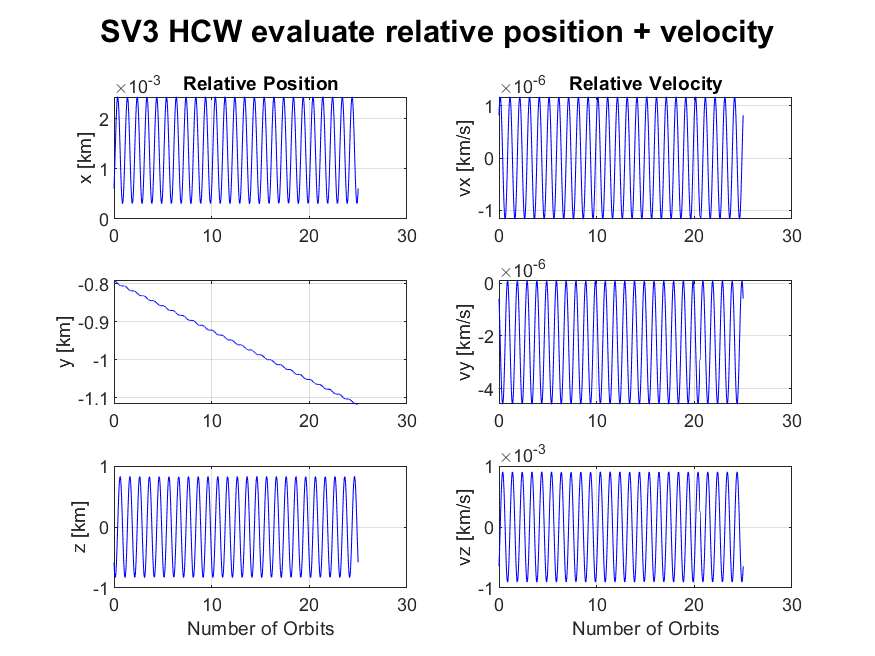
\includegraphics[width=0.7\linewidth]{sim/figures/PS3/HCW_pos_vel_SV2.png}
    \caption{Relative position and velocity of SV2 in the chief's RTN frame, evaluated using HCW equations.}
    \label{fig:hcw_sv2_pos_vel}
\end{figure}

\begin{figure}[htpb]
    \centering
    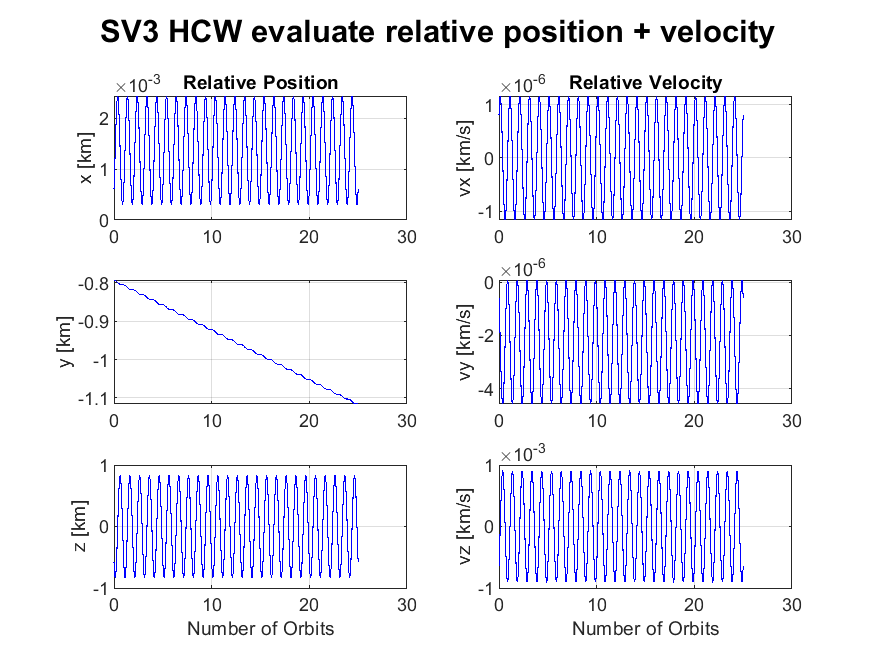
\includegraphics[width=0.7\linewidth]{sim/figures/PS3/HCW_pos_vel_SV3.png}
    \caption{Relative position and velocity of SV3 in the chief's RTN frame, evaluated using HCW equations.}
    \label{fig:hcw_sv2_pos_vel}
\end{figure}

\begin{figure}[htpb]
    \centering
    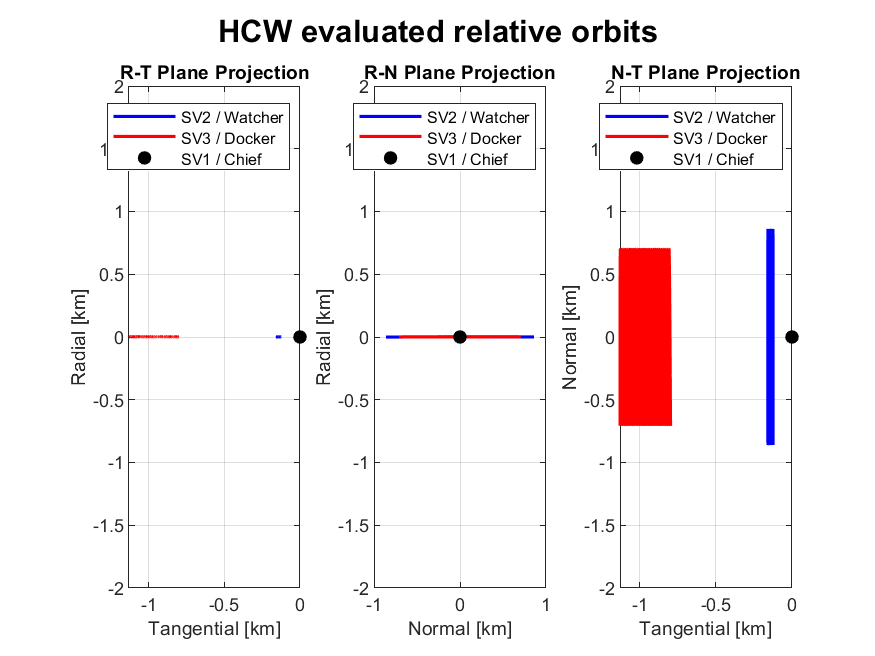
\includegraphics[width=0.7\linewidth]{sim/figures/PS3/RTN_projections_HCW.png}
    \caption{RTN Projections of SV2 and SV3 trajectories calculating using HCW}
    \label{fig:hcw_projections}
\end{figure}

\begin{figure}[htpb]
    \centering
    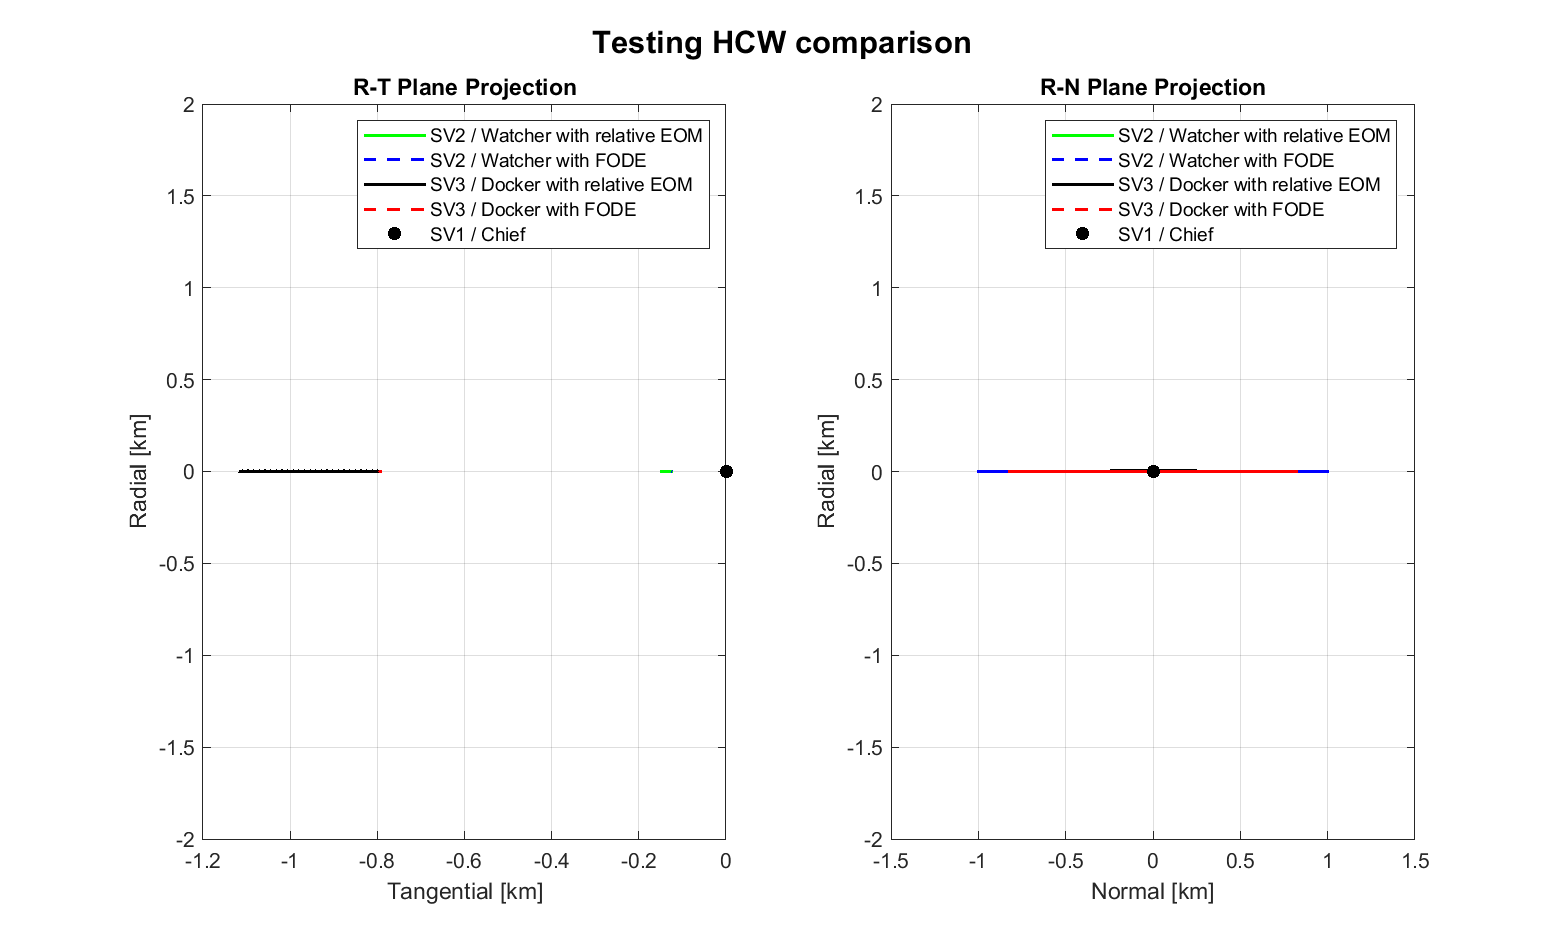
\includegraphics[width=0.7\linewidth]{sim/figures/PS3/RTN_projections_HCW_comparison.png}
    \caption{RTN Projections of SV2 and SV3 comparison between HCW and FERM.}
    \label{fig:hcw_comparisons_projections}
\end{figure}

\begin{figure}[htpb]
    \centering
    \begin{subfigure}[t]{0.45\linewidth}
        \centering
        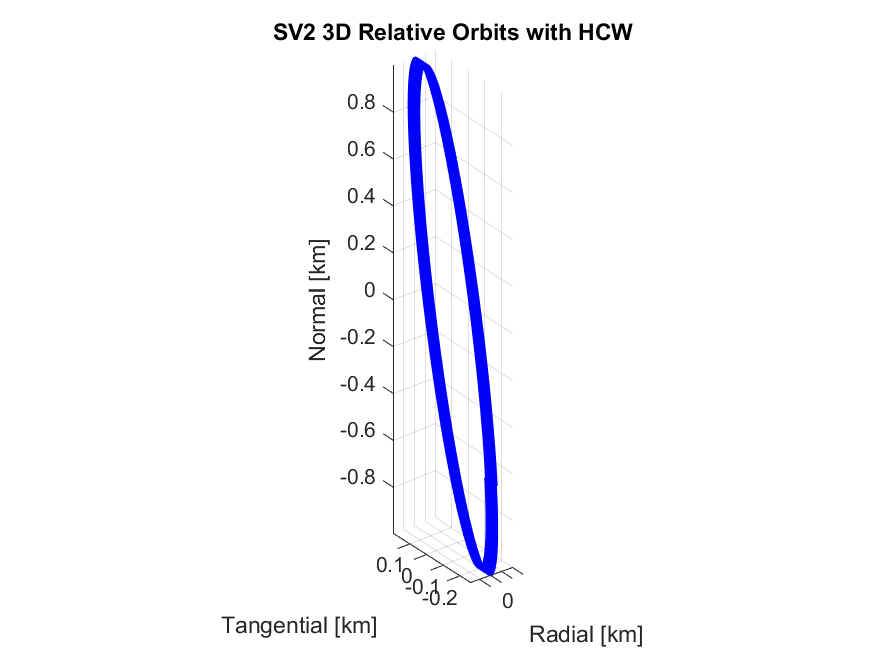
\includegraphics[width=1.2\linewidth]{sim/figures/PS3/3D_HCW_orbit_SV2.png}
        \caption{SV2-HCW Orbit}
        \label{fig:hcw_sv2}
    \end{subfigure}%
    \begin{subfigure}[t]{0.45\linewidth}
        \centering
        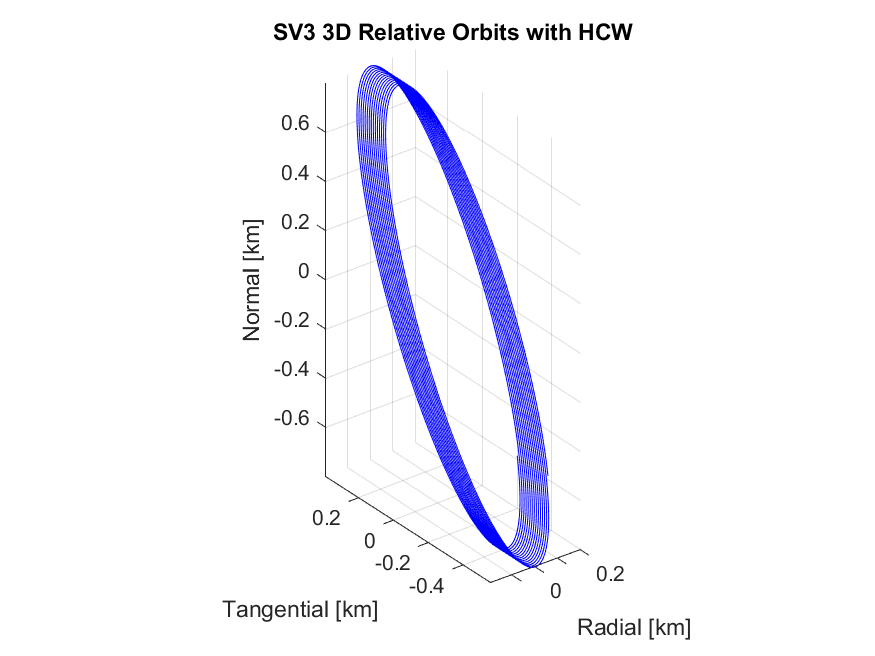
\includegraphics[width=1.2\linewidth]{sim/figures/PS3/3D_HCW_orbit_SV3.png}
        \caption{SV3-HCW Orbit}
        \label{fig:hcw_sv3}
    \end{subfigure}
    \caption{3D HCW-relative orbits of SV2 and SV3.}
    \label{fig:hcw_3d_side_by_side}
\end{figure}

\subsubsection{Analysis of HCW Solution Behavior}

\newpage

\subsection{We are Close in Eccentric Orbits}
\subsubsection{Initial Conditions for Tschauner-Hempel Equations}
Now, we turn our analysis to eccentric orbits, where relative motion is described by the Tschauner-Hempel (TH) equations. The TH equations can be solved using the Yamanaka-Ankersen (YA) model. We will use the same initial conditions for the absolute and relative states as with HCW, except now the chief's orbit has an eccentricity of 0.15. The ROE for SV2 and SV3 remain the same as outlined in Table \ref{{tab:relative_oe_hcw}}, as these initial conditions also lie whtin the range of validity of the TH equations. Specifically, the chief and deputy have equal semi-major axes and the the maximum separation between spacecraft is small relative to the minimum distance from the primary attractor center. 

\subsection{YA Integration Constants}
From these chosen initial conditions, the 6 integration constants of the YA solution can be computed through the following process.

Willis outlines the transformation matrices ($A,B$) from YA integration constants to RTN position and velocity of the deputy \cite{willis2023analytical}. These matrices can be inverted to instead go from initial RTN position and velocity to YA integration constants. 

YA defines the following expressions:
\begin{align*}
n &= \sqrt{\frac{\mu_{\text{earth}}}{a^3}} \\
\eta &= \sqrt{1 - e^2} \\
\tau &= \frac{nt}{\eta^3}\\
k &= 1 + e \cos(f) \\
k' &= -e \sin(f)
\end{align*}

And the following transformation components:
\begin{align*}
\psi_{x1} &= \frac{1}{k} + \frac{3}{2}k' \tau, &
\psi_{x2} &= \sin(f), &
\psi_{x3} &= \cos(f) \\
\psi_{y1} &= -\frac{3}{2}k\tau, &
\psi_{y2} &= \left(1 + \frac{1}{k}\right)\cos(f), &
\psi_{y3} &= -\left(1 + \frac{1}{k}\right)\sin(f), &
\psi_{y4} &= \frac{1}{k} \\
\psi_{z5} &= \frac{1}{k}\sin(f), &
\psi_{z6} &= \frac{1}{k}\cos(f)
\end{align*}

And their respective derivatives:
\begin{align*}
\psi_{x1}' &= \frac{k'}{2} - \frac{3}{2}k^2(k - 1)\tau, &
\psi_{x2}' &= k^2 \cos(f), &
\psi_{x3}' &= -k^2 \sin(f) \\
\psi_{y1}' &= -\frac{3}{2}\left(k + k^2k'\tau\right), &
\psi_{y2}' &= -(k^2 + 1)\sin(f), &
\psi_{y3}' &= -e - (k^2 + 1)\cos(f), &
\psi_{y4}' &= -k' \\
\psi_{z5}' &= e + \cos(f), &
\psi_{z6}' &= -\sin(f)
\end{align*}

And finally the full transformation matrices:
\begin{align*}
A &= 
\begin{bmatrix}
a\eta^2 I_{3 \times 3} & 0 \\
0 & \frac{a n}{\eta} I_{3 \times 3}
\end{bmatrix}
\end{align*}

\begin{align*}
B &=
\begin{bmatrix}
\psi_{x1} & \psi_{x2} & \psi_{x3} & 0 & 0 & 0 \\
\psi_{y1} & \psi_{y2} & \psi_{y3} & \psi_{y4} & 0 & 0 \\
0 & 0 & 0 & 0 & \psi_{z5} & \psi_{z6} \\
\psi_{x1}' & \psi_{x2}' & \psi_{x3}' & 0 & 0 & 0 \\
\psi_{y1}' & \psi_{y2}' & \psi_{y3}' & \psi_{y4}' & 0 & 0 \\
0 & 0 & 0 & 0 & \psi_{z5}' & \psi_{z6}'
\end{bmatrix}
\end{align*}

We then invert the transformation matrices to solve for the initial conditions:
\[
K = (A B)^{-1} \cdot \begin{bmatrix}
x_0 \\ y_0 \\ z_0 \\ \dot{x}_0 \\ \dot{y}_0 \\ \dot{z}_0
\end{bmatrix}
\]

Note that in solving this equation, $\tau$ will be zero because our initial time is 0. For our chosen initial conditions, the integration constants computed are provided in Table \ref{tab:integration_constants_HCW}.

\begin{table}[ht]
    \centering
    \renewcommand{\arraystretch}{1.2}
    \begin{tabular}{c c c}
        \toprule
        \textbf{Constant} & \textbf{SV2} & \textbf{SV3} \\
        \midrule
        $K_1$ & $-1.5886\cdot10^{-8}$ & $-1.0799\cdot10^{-8}$ \\
        $K_2$ & $3.7051\cdot10^{-6}$ & $2.9694\cdot10^{-6}$ \\
        $K_3$ & $-1.4750\cdot10^{-5}$& $-2.9477\cdot10^{-5}$\\
        $K_4$ & $8.4251\cdot10^{-7}$ & $6.7435\cdot10^{-7}$ \\
        $K_5$ & $1.4401\cdot10^{-4}$ & $1.1521\cdot10^{-4}$ \\
        $K_6$ & $3.8971\cdot10^{-8}$ & $3.0781\cdot10^{-8}$ \\
        \bottomrule
    \end{tabular}
    \caption{Integration Constants for SV2 and SV3 Used in HCW Analytical Solution}
    \label{tab:integration_constants_HCW}
\end{table}

\subsection{Relative State Propagation Using YA Solution}
We use the same propagation strategy as with the HCW solution, except now using the YA integration constants and STM. 


\newpage
\section{Problem Set 4}
\subsection{These are Relative Orbits!}

\subsubsection{Initial Conditions for the Chief} 
The osculating initial conditions for the chief are the same as outlined in Table \ref{tab:abs_oe}. We chose to remain with the same initial chief conditions since they are well within the range of the HCW equations, with an eccentricity much less than 1. 

\subsubsection{Initial Conditions for the Deputy} \label{sec:ic_for_pset4}

We set the new initial conditions for the deputy based on the following given values. Since we are only considering one set of provided initial conditions in this section of the report, we only consider a single deputy (SV2), as the results for SV3 would be identical if given the same initial conditions.

\[
a_c (\delta a, \delta \lambda, \delta e_x, \delta e_y, \delta i_x, \delta i_y) = (0,\ 100,\ 50,\ 100,\ 30,\ 200)~\text{m}
\]

\subsubsection{Numerical Integration of Chief and Deputy}
From these initial conditions, we can perform a numerical integration of the equations of motion for the chief and deputy with position and velocity as state variables. This process is outlined in Section \ref{sec:rel_FODE_num_int}. The simulation was repeated two times with the same initial conditions: with and without J2 effects. Then the osculating and mean absolute and relative quasi-non-singular orbital elements were computed. The numerical integration was done with osculating inputs and outputs, thus Brower's Theory was used to convert the osculating quantities to mean quantities. 

Figure \ref{fig:osc_OE} shows the osculating quasi-non-singular orbital elements, while Figure \ref{fig:mean_OE} shows the mean quasi-non-singular orbital elements. As expected, both the osculating and mean elements showcase the secular effects of J2 on both the components of the eccentricity vector and RAAN. There is also a drift in true longitude, but it is so small that it is not observable on these figures. The equations governing these drifts and a discussion around them can be found in Section \ref{sec:osc_mean_J2}.

Also as expected, the osculating quantities also showcase periodic effects of J2 on eccentricity, inclination, and semi-major axis. Note that there are minor offsets between the mean and osculating quantities with J2 effects in semi-major axis, eccentricity, and inclination, which are introduced by the approximate inverse transformation done in Brower's Theory during the conversion. Without J2 effects, the mean and osculating quantities line up exactly, because by definition, they are equivalent when there are no perturbations. 

\begin{figure}[H]
    \centering
    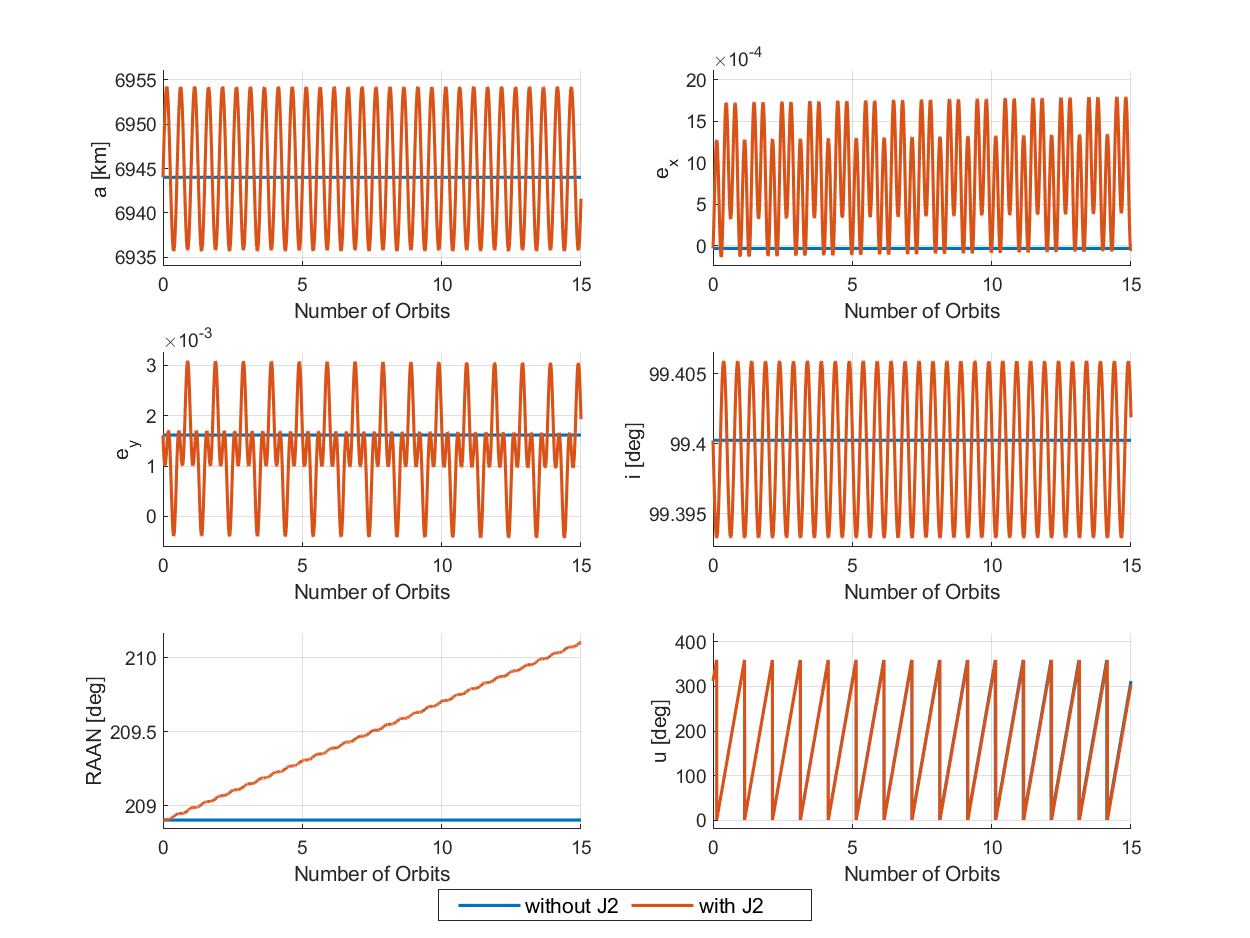
\includegraphics[width=0.75\linewidth]{sim/figures/PS4/OE_abs_osc_SV2.png}
    \caption{Osculating quasi-non-singular orbital elements}
    \label{fig:osc_OE}
\end{figure}

\begin{figure}[H]
    \centering
    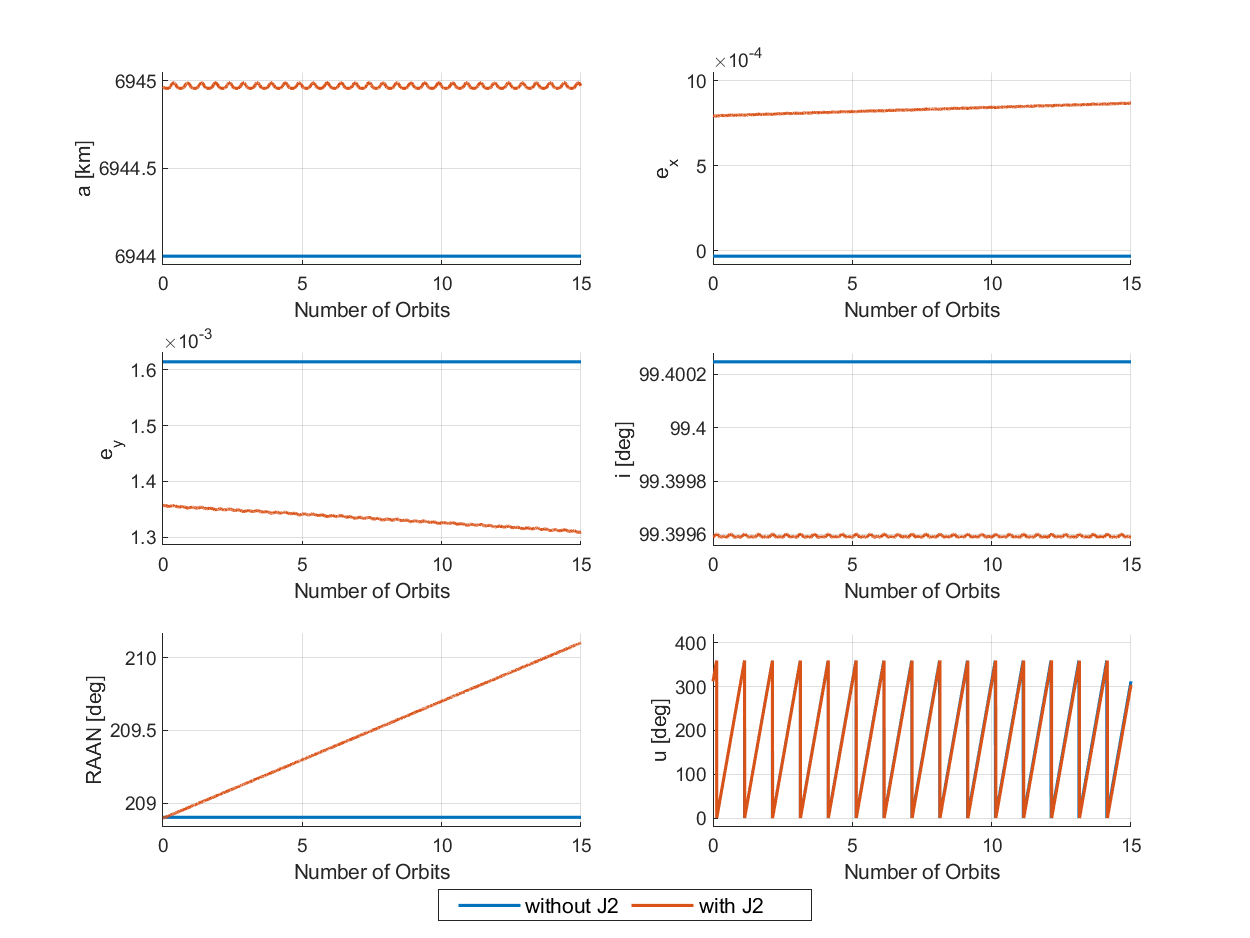
\includegraphics[width=0.75\linewidth]{sim/figures/PS4/OE_abs_mean_SV2.png}
    \caption{Mean quasi-non-singular orbital elements}
    \label{fig:mean_OE}
\end{figure}

Similarly, Figure \ref{fig:osc_ROE} shows the osculating relative quasi-non-singular orbital elements, while Figure \ref{fig:mean_ROE} shows the mean relative quasi-non-singular orbital elements. Again, as expected, J2 effects are observed in $\delta \lambda$, the phase of the eccentricity vector, and $\delta i_y$

\begin{figure}[H]
    \centering
    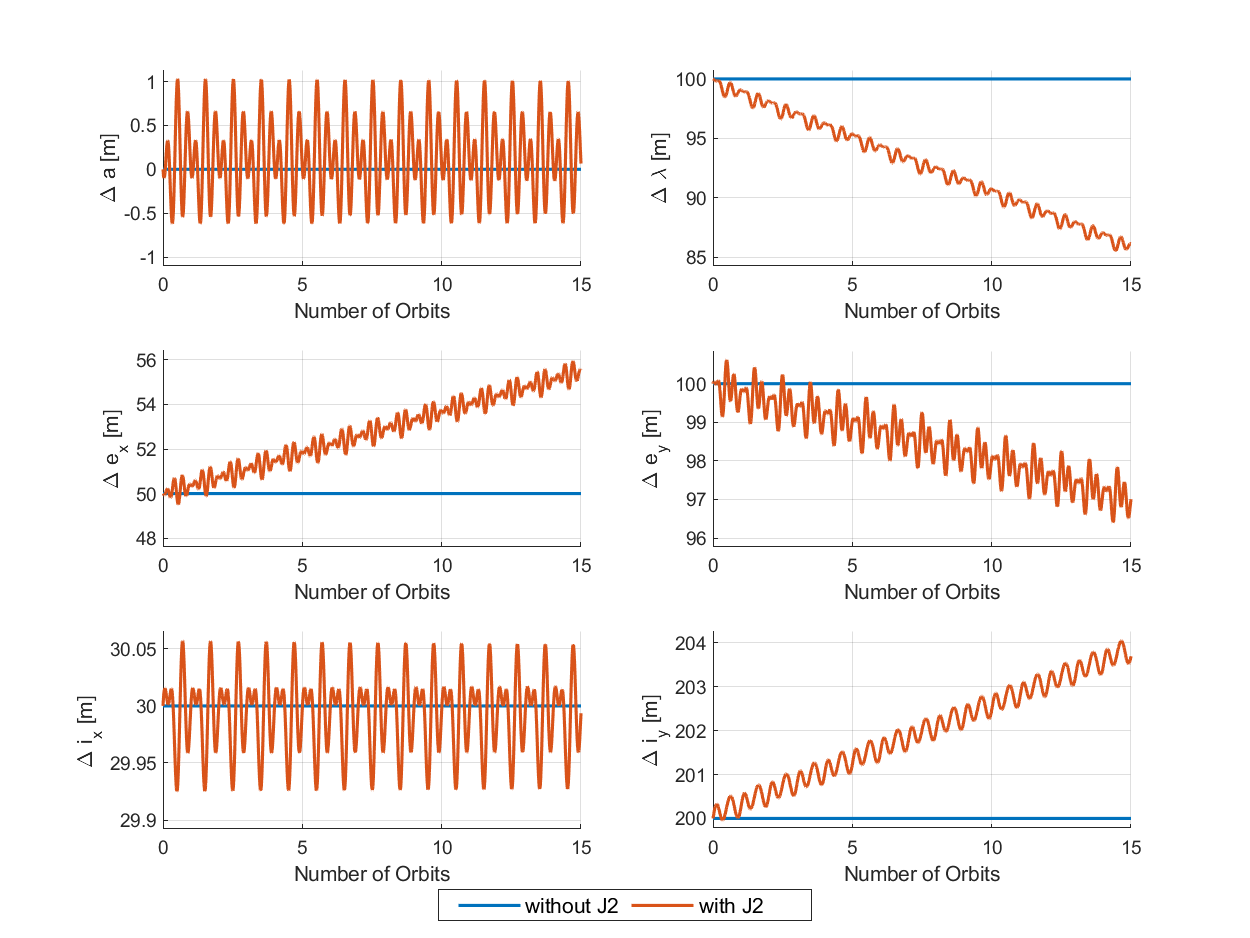
\includegraphics[width=0.75\linewidth]{sim/figures/PS4/ROE_osc_SV2.png}
    \caption{Osculating relative quasi-non-singular orbital elements}
    \label{fig:osc_ROE}
\end{figure}

\begin{figure}[H]
    \centering
    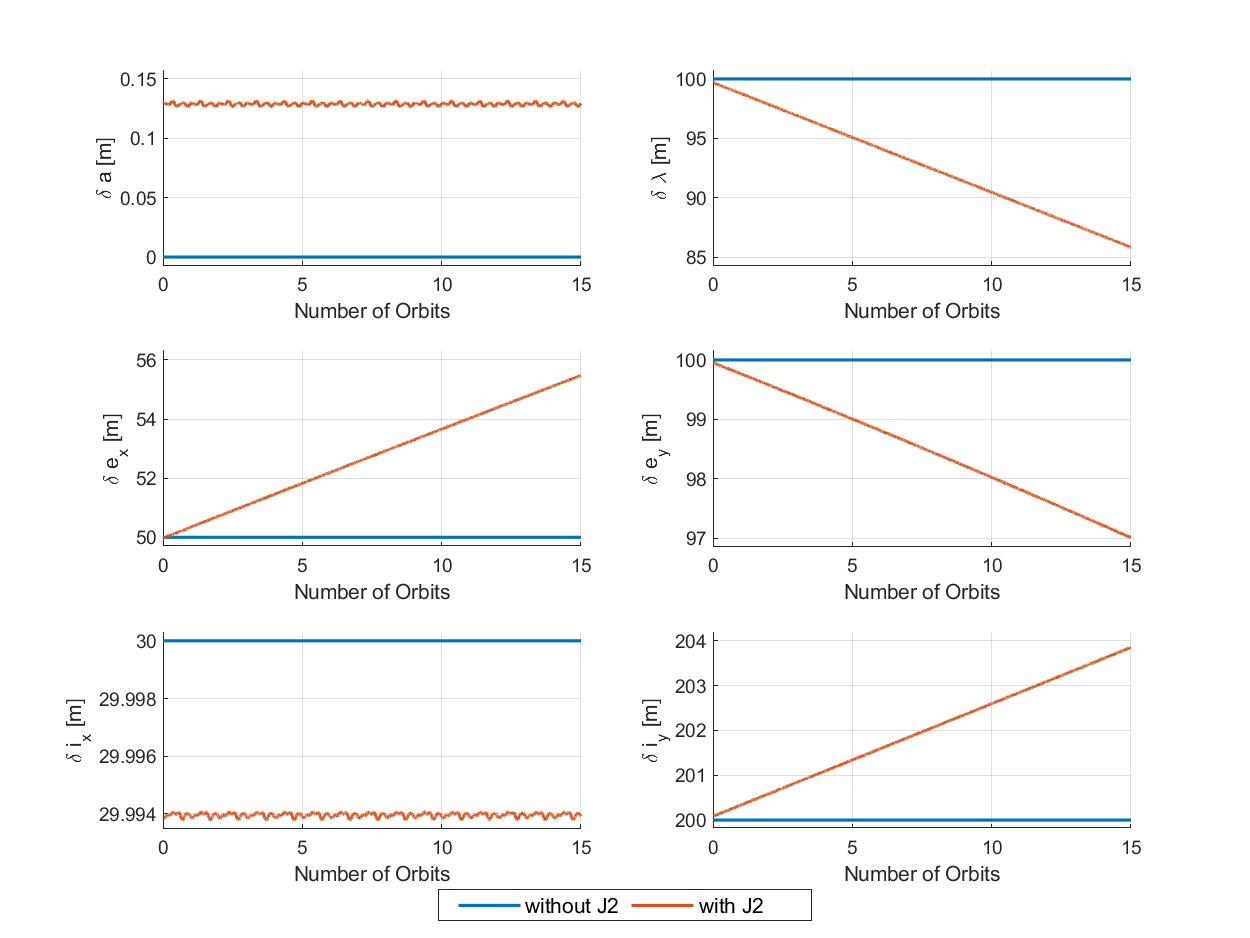
\includegraphics[width=0.75\linewidth]{sim/figures/PS4/ROE_mean_SV2.png}
    \caption{Mean relative quasi-non-singular orbital elements}
    \label{fig:mean_ROE}
\end{figure}

\subsubsection{J2 perturbations in RTN Frame}



\subsubsection{J2 perturbations in ROE space}

\subsubsection{Maneuver to remove J2 secular effects}

In the quasi-nonsingular relative orbital elements, there are drifts seen in the eccentricity vector $\delta e$, the inclination vector $\delta i$ (specifically the y-component $\delta i_y$), and the mean longitude $\delta \lambda$. The differential J2 effects for near-circular orbits is given by
\begin{align}
    \frac{d \varphi'}{d u} &= \frac{3}{2} \gamma (5\cos^2(i_c) - 1) \\
    \frac{d \delta i_y}{d u} &= 3\gamma \sin^2(i_c) \delta i_x \label{eq:drift_in_rel_i} \\
    \frac{d \delta \lambda}{d u} &= -\frac{21}{2}\left(\gamma \sin(2i_c)\delta i_x 
+ \frac{1}{7} \delta a\right) \label{eq:drift_in_lambda_rel}\\
    \text{where} \quad \gamma  &= \frac{J_2 R_E^2}{2 a^2 (1 - e)^2}
\end{align}
Here, the $\varphi$ is the angle of the eccentricity vector $\delta e$, i.e. $\varphi = \tan^{-1}\left(\frac{\delta e_y}{\delta e_x}\right)$. So, we see that the drift in the eccentricity vector is circular rather than secular. Therefore, to eliminate the secular drift we just need to eliminate the secular effects in the inclination vector and the mean longitude.

From Equation \ref{eq:drift_in_rel_i}, we see that one way to remove this differential effect in the inclination vector is by setting $\delta i_x = 0$. From Equation \ref{eq:quasi_nonsign_roe}, $\delta i_x = 0 \implies i_t = i_o$, or in other words the deputy satellite and the chief satellite have the same orbital inclination. 

To completely remove the drift in the mean longitude based on Equation \ref{eq:drift_in_lambda_rel}, we would need to not only set $\delta i_x = 0$ but also  $\delta a = 0$. 

Based on the given initial conditions in Section \ref{sec:ic_for_pset4}, we assume that the $\delta a = 0$ already. So the maneuver would mainly be to remove the inclination difference. 

The optimal location (minimum $\Delta v$) to produce an orbital inclination change is at the ascending node of the orbit, i.e. when $u_M = TODO$, and with the TODO TODO TODO. Direction is perpendicular?

TODO: Could also do a more in-depth derivation from the STM for the delta lambda terms.

\subsubsection{Simulation with new initial conditions that don't have secular effects}

We set the initial condition $\delta i_x = 0$ to remove secular effects. With this, we get the relative orbital elements over time shown in Figure \ref{fig:rel_roe_no_drift}.

\begin{figure}[htpb]
    \centering
    \includegraphics[width=0.5\linewidth]{}
    \caption{Relative orbital elements with initial conditions set to remove the }
    \label{fig:rel_roe_no_drift}
\end{figure}

\subsubsection{Analytical Solution for J2 on Relative Orbital Elements}

\begin{align*}
\Phi^{J_2}_{\text{qns}}(\alpha_c(t_i), \tau) &=
\begin{bmatrix}
1 & 0 & 0 & 0 & 0 & 0 \\
-\left( \frac{3}{2}n + \frac{7}{2} \kappa E P \right)\tau & 1 & \kappa e_{x_i} F G P \tau & \kappa e_{y_i} F G P \tau & -\kappa F S \tau & 0 \\
\frac{7}{2} \kappa e_{y_f} Q \tau & 0 & \cos(\dot{\omega} \tau) - 4\kappa e_{x_i} e_{y_f} G Q \tau & -\sin(\dot{\omega} \tau) - 4\kappa e_{y_i} e_{y_f} G Q \tau & 5\kappa e_{y_f} S \tau & 0 \\
-\frac{7}{2} \kappa e_{x_f} Q \tau & 0 & \sin(\dot{\omega} \tau) + 4\kappa e_{x_i} e_{x_f} G Q \tau & \cos(\dot{\omega} \tau) + 4\kappa e_{y_i} e_{x_f} G Q \tau & -5\kappa e_{x_f} S \tau & 0 \\
0 & 0 & 0 & 0 & 1 & 0 \\
\frac{7}{2} \kappa S \tau & 0 & -4 \kappa e_{x_i} G S \tau & -4 \kappa e_{y_i} G S \tau & 2 \kappa T \tau & 1
\end{bmatrix}
\begin{bmatrix}
\delta a \\
\delta \lambda \\
\delta e_x \\
\delta e_y \\
\delta i_x \\
\delta i_y
\end{bmatrix}
\end{align*}

\vspace{1em}

\noindent
\textbf{Eccentricity dependent parameters:}
\begin{align*}
\eta &= \sqrt{1 - e^2} &
\kappa &= \frac{3}{4} \frac{J_2 R_E^2 \sqrt{\mu}}{a^{7/2} \eta^4} &
E &= 1 + \eta \\
F &= 4 + 3\eta &
G &= \frac{1}{\eta^2}
\end{align*}

\vspace{1em}

\noindent
\textbf{Inclination dependent parameters:}
\begin{align*}
P &= 3\cos^2(i) - 1 &
Q &= 5\cos^2(i) - 1 &
R &= \cos(i) \\
S &= \sin(2i) &
T &= \sin^2(i) &
U &= \sin(i) \\
V &= \tan(i/2) &
W &= \cos^2(i/2)
\end{align*}

\cite{koenig2017new}
\newpage
\section{Problem Set 5}
\subsection{Control Objectives} \label{sec:control_objectives}
\subsubsection{Operational Modes}
The ultimate goal of our formation is to demonstrate on-orbit servicing of an uncontrollable target spacecraft with a swarm of one docking satellite and one observing satellite. Specifically, the Target spacecraft (SV1) has no maneuvering capabilities as it has run out of propellant, and our formation is aiming to refuel it. As such, SV1 will act as the origin of the RTN frame and remain there throughout all of our operational modes. The Watcher spacecraft (SV2) has sensing capabilities, including optical cameras such as those in the NASA Starling mission, which will be used to inspect the Target and estimate its pose for servicing purposes. The Docker spacecraft (SV3) also has optical sensors that will aid in this inspection, but also play a crucial role in proximity and docking operations. Our formation aims to demonstrate a significant advance in on-orbit pose estimation and characterization of objects, along with improved docking operations through the use of multiple spacecraft with a variety of sensor modalities. 

In order to achieve this, the significant operational modes of our formation are as follows: 

\begin{enumerate}
\item \textbf{Initial Checkout Mode} - Initial checkout of Target spacecraft with both Watcher and Docker less than a kilometer and more than 200 meters away at closest approach to allow for vision-based sensing
\item \textbf{Approach Mode} - Docker approaches the Target while Watcher watches from the same distance. This mode runs until the Docker is approximately 10 meters away from the Target
\item \textbf{Proximity Operations Mode} - Docker completes final approach Target while Watcher watches
\item \textbf{Docked Mode} - Docker docks and services Target while Watcher watches
\item \textbf{Station Keeping Mode} - Watcher and Target stay within prescribed limits of relative eccentricity and relative inclination to remain passively safe. This mode will be applied whenever the formation is not reconfiguring. 
\end{enumerate}

\subsubsection{Operational Mode ROEs}
The absolute motion of our spacecraft is not the focus, as our formation is purely concerned with servicing a satellite. As such, all of the operational modes are defined as deputy ROEs as follows. Note that the Approach mode was split into two separate waypoints (Mode 2 and Mode 3) to better illustrate the reconfiguration. 

\begin{table}[h!]
\centering
\begin{tabular}{|c|rrrrrr|rrrrrr|}
\hline
\textbf{Mode} & \multicolumn{6}{c|}{\textbf{SV2 (m)}} & \multicolumn{6}{c|}{\textbf{SV3 (m)}} \\
\cline{2-13}
 & $d_a$ & $d_\lambda$ & $d_{e_x}$ & $d_{e_y}$ & $d_{i_x}$ & $d_{i_y}$ 
 & $d_a$ & $d_\lambda$ & $d_{e_x}$ & $d_{e_y}$ & $d_{i_x}$ & $d_{i_y}$ \\
\hline
1 & 0 & 0 & 0 & 300 & 0 & 300 & 0 & 0 & 0 & 250 & 0 & -250 \\
2 & 0 & 0 & 0 & 300 & 0 & 300 & 0 & 0 & 0 & 100 & 0 & -100 \\
3 & 0 & 0 & 0 & 300 & 0 & 300 & 0 & 0 & 0 & 10  & 0 & -10 \\
4 & 0 & 0 & 0 & 300 & 0 & 300 & 0 & 0 & 0 & 1   & 0 & -1 \\
\hline
\end{tabular}
\caption{Relative Orbital Element Modes for SV2 and SV3 (scaled by $a_c$)}
\label{tab:roe_modes}
\end{table}

These ROE values were chosen to meet the minimum separation requirements outlined above, by using the following equation:

\begin{align}
R_{\min} &= \frac{\sqrt{2} \cdot a \cdot |\delta e \cdot \delta i|}%
{\sqrt{(\delta e)^2 + (\delta i)^2 + |\delta e + \delta i| \cdot |\delta e - \delta i|}}
\end{align} \label{eqn:roe_spacing}

Plotting this equation in 3D shows that the minimum distance is dominated by the minimum of the given $\delta e$ and $\delta i$, as shown by Figure \ref{fig:min_dist_contour}.
\begin{figure}[H]
    \centering
    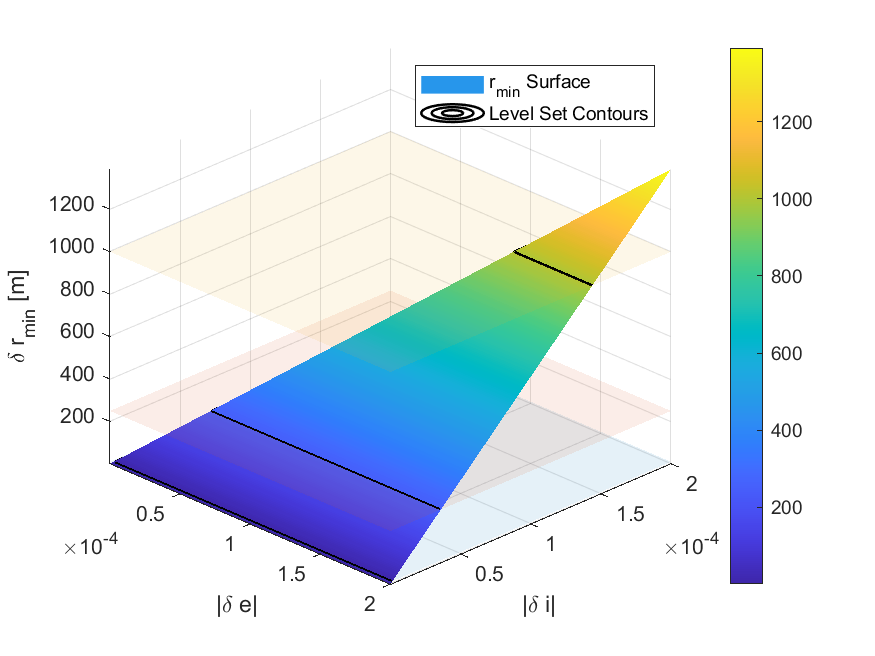
\includegraphics[width=0.75\linewidth]{sim/figures/PS5/min_dist_contour.png}
    \caption{Minimum distance contour over relative eccentricity and relative inclination}
    \label{fig:min_dist_contour}
\end{figure}
As such, $\delta e$ and $\delta i$ were chosen to be equal in magnitude for both SV2 and SV3 in order to give circular relative motion, which is helpful for maintaining the same distance throughout an orbit for the vision-based sensing on both spacecraft. Additionally, $\delta e$ and $\delta i$ were chosen to be antiparallel for SV3 (Docker) and parallel for SV2 (Watcher) to ensure that the Docker never blocks the Watcher's view of the Target by tilting the Docker's relative orbit perpendicular to the Watcher's.

\subsubsection{Formation Keeping Control Requirements}
For each station keeping mode, a keep-in region was defined for the relative eccentricity and relative inclination in order to ensure passive safety and maintain the allowable separations defined earlier. Due to the small size of the relative eccentricity and relative inclination vectors during our operational modes, a tight keep-in region of a circle with a 1-meter radius was used. 

This tight keep-in region dictates a tight relative position knowledge requirement: the Watcher's knowledge should be less than a meter and the Docker's should be less than a centimeter in order to allow for successful docking and servicing. Similarly, the velocity estimation of the Docker should be on order of mm/s.

Additionally, the actuation needed will be low-thrust, high-preicison with a low impulse bit on the order of mm/s, such as a cold gas thruster. Short, impulsive bursts will be used so to not disturb the attitude of the Docker and allow for precise control. 


\subsubsection{Reconfiguration Control Requirements}
For reconfiguration, there must always be passive safety, which is achieved through aligning the relative eccentricity and relative inclination vectors. Additionally the time to reconfigure, given in number of orbits, is prescribed for each mode below. These numbers were chosen to best illustrate the control behavior. In practice, the Approach Mode would take the longest time, especially in proximity operations where the maneuvers are small and need to be precise. 

\begin{table}[h!]
\centering
\begin{tabular}{|c|c|}
\hline
\textbf{Phase} & \textbf{Number of Orbits} \\
\hline
Mode 2 & 2 \\
Station-Keeping 2 & 3 \\
Mode 3 & 2 \\
Station-Keeping 3 & 3 \\
Mode 4 & 2 \\
\hline
\end{tabular}
\caption{Number of orbits spent in each mode and station-keeping phase} \label{tab:mode_durations}
\end{table}

\subsubsection{Choice of Actuators}
Two different types of actuators will be used. The first will be higher-thrust and lower specific impulse chemical propulsion for station keeping, phasing, and the approach. Electric propulsion is also an option here as it has higher specific impulse, but will not be used for now as impulsive delta-v's are simpler to model. The second kind of actuator used with be lower-thrust propulsion, such as cold-gas thrusters. These will be used for proximity and docking operations, as fine and accurate thrust control with small impulse bits is required. Cold gas thrusters will be used instead of hydrazine thrusters since they are less hazardous to work with. 

\subsubsection{Absolute and Relative Orbit Dynamics Models}
Two dynamics models are needed: the first will be the ground-truth and the second will actually run onboard the computationally-limited spacecraft. The absolute ground-truth will be given by numerical integration of the Fundamental Orbital Differential Equation (FODE) with J2 effects for the chief and both deputies. The relative ground-truth will be calculated by taking the differences in the absolute states and converting to the RTN and ROE representations. The onboard dynamics model cannot perform numerical integration as this would be too computationally-expensive. Instead, the absolute and onboard dynamics will be given by the analytical STM with J2 for ROE as outlined in Section \ref{sec:j2_analytical_roe}, which still needs to provide accuracy as it will be used for control. 

Implementing the ground-truth model in open-loop shows each desired mode in the RTN planes as shown in Figures \ref{fig:mode_1_rtn}, \ref{fig:mode_2_rtn}, \ref{fig:mode_3_rtn}. Note that Mode 4 is not shown because SV3 does not appear in the plots due to its ROE all being 0. This ground-truth model exhibits expected J2 perturbations with a drifting relative perigee. Also note how the inclinations of the relative orbits are offset in the NT projection due to the design choice of antiparallel relative eccentricity and relative inclination vectors of SV3. All of these modes exhibit passive safety as well. 

% --- Mode 1 ---
\begin{figure}[H]
    \centering
    \begin{subfigure}[b]{0.32\linewidth}
        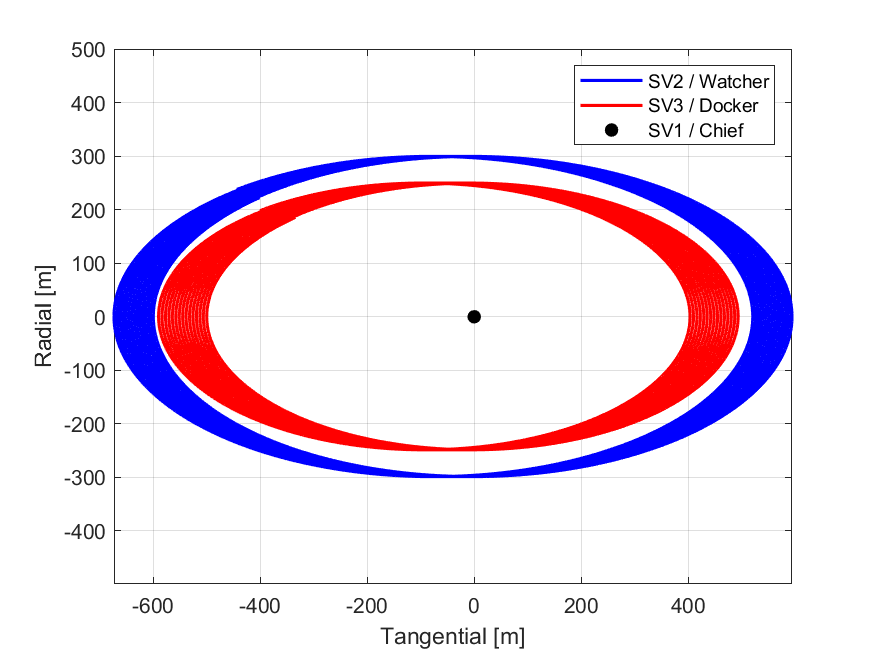
\includegraphics[width=\linewidth]{sim/figures/PS5/mode_1_RTN.png_RT.png}
        \caption{RT Projection}
        \label{fig:mode_1_rt}
    \end{subfigure}
    \begin{subfigure}[b]{0.32\linewidth}
        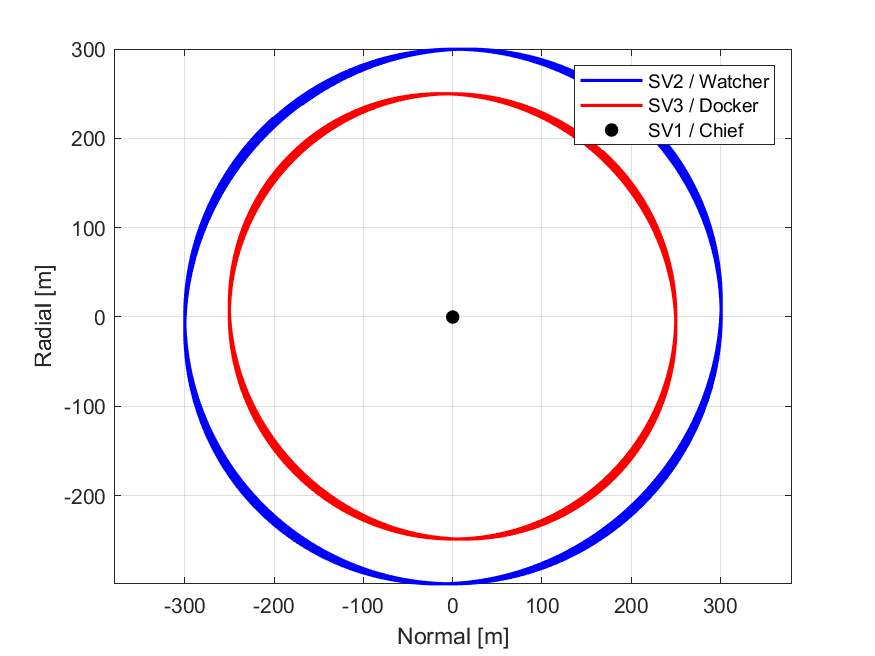
\includegraphics[width=\linewidth]{sim/figures/PS5/mode_1_RTN.png_RN.png}
        \caption{RN Projection}
        \label{fig:mode_1_rn}
    \end{subfigure}
    \begin{subfigure}[b]{0.32\linewidth}
        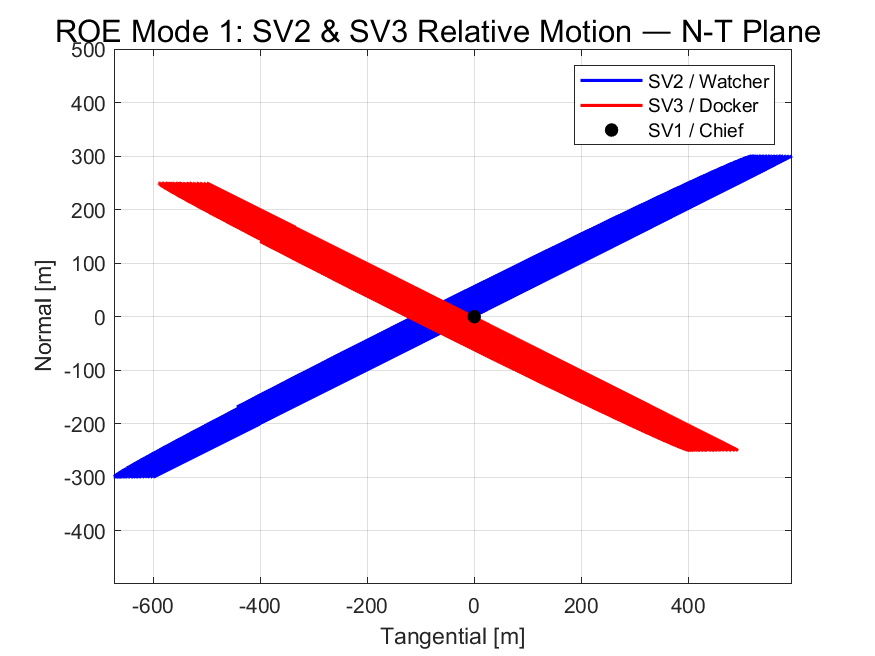
\includegraphics[width=\linewidth]{sim/figures/PS5/mode_1_RTN.png_NT.png}
        \caption{NT Projection}
        \label{fig:mode_1_nt}
    \end{subfigure}
    \caption{Mode 1 RTN Projections}
    \label{fig:mode_1_rtn}
\end{figure}

% --- Mode 2 ---
\begin{figure}[H]
    \centering
    \begin{subfigure}[b]{0.32\linewidth}
        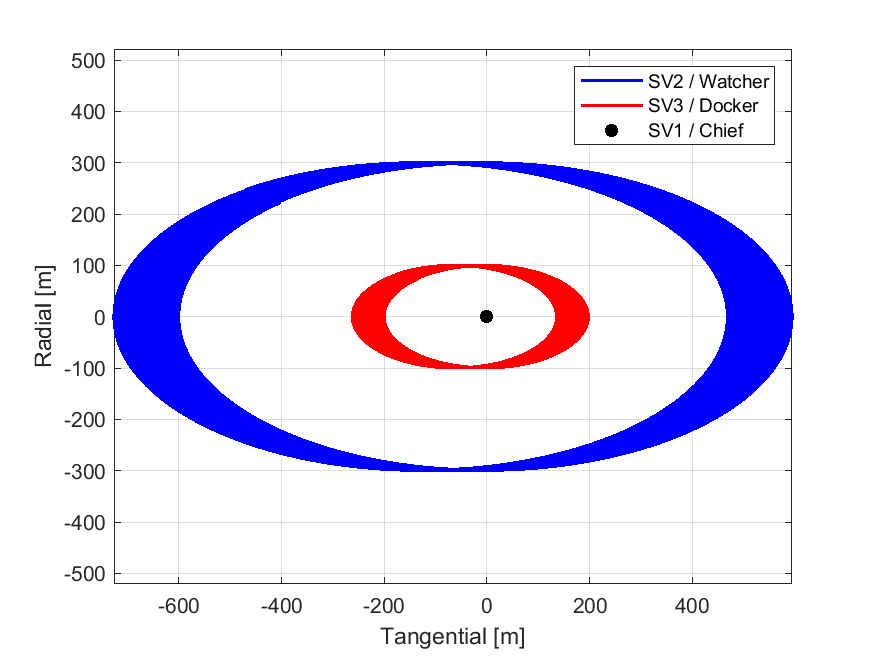
\includegraphics[width=\linewidth]{sim/figures/PS5/mode_2_RTN.png_RT.png}
        \caption{RT Projection}
        \label{fig:mode_2_rt}
    \end{subfigure}
    \begin{subfigure}[b]{0.32\linewidth}
        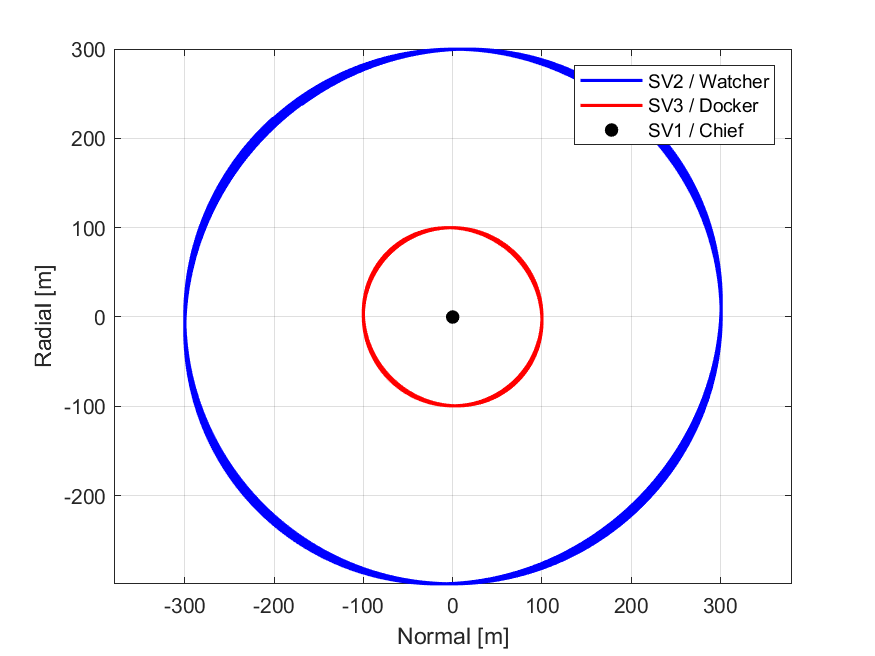
\includegraphics[width=\linewidth]{sim/figures/PS5/mode_2_RTN.png_RN.png}
        \caption{RN Projection}
        \label{fig:mode_2_rn}
    \end{subfigure}
    \begin{subfigure}[b]{0.32\linewidth}
        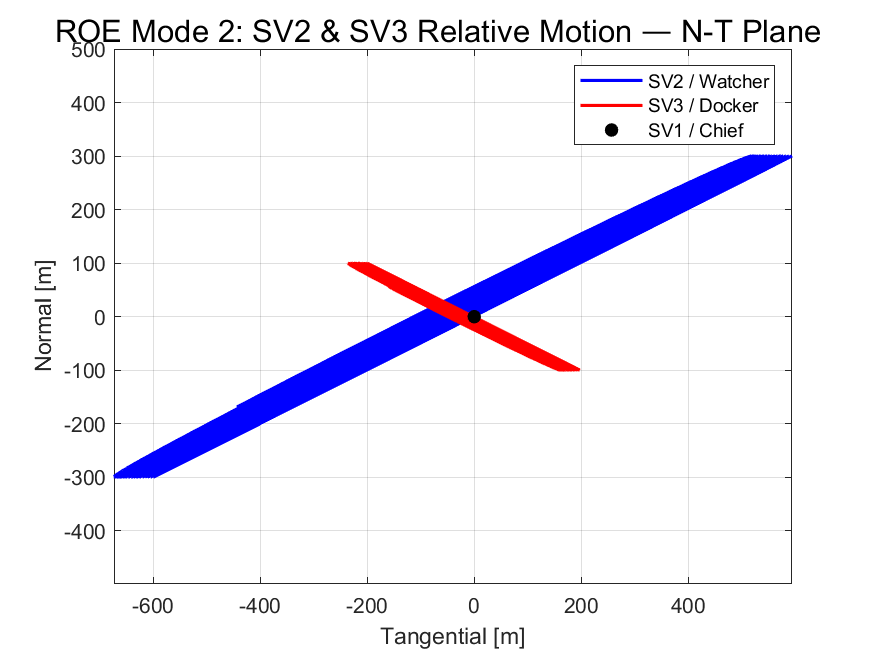
\includegraphics[width=\linewidth]{sim/figures/PS5/mode_2_RTN.png_NT.png}
        \caption{NT Projection}
        \label{fig:mode_2_nt}
    \end{subfigure}
    \caption{Mode 2 RTN Projections}
    \label{fig:mode_2_rtn}
\end{figure}

% --- Mode 3 ---
\begin{figure}[H]
    \centering
    \begin{subfigure}[b]{0.32\linewidth}
        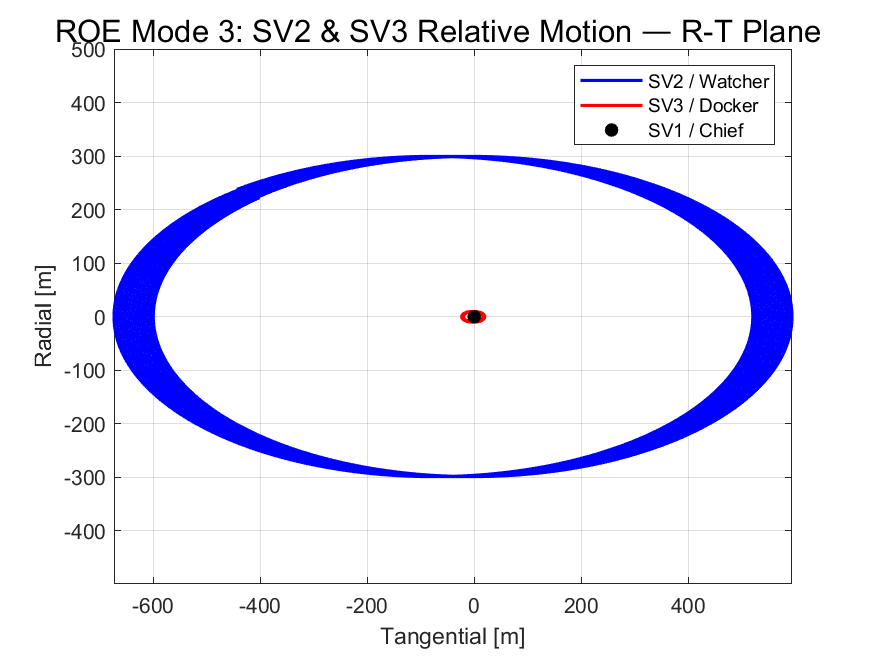
\includegraphics[width=\linewidth]{sim/figures/PS5/mode_3_RTN.png_RT.png}
        \caption{RT Projection}
        \label{fig:mode_3_rt}
    \end{subfigure}
    \begin{subfigure}[b]{0.32\linewidth}
        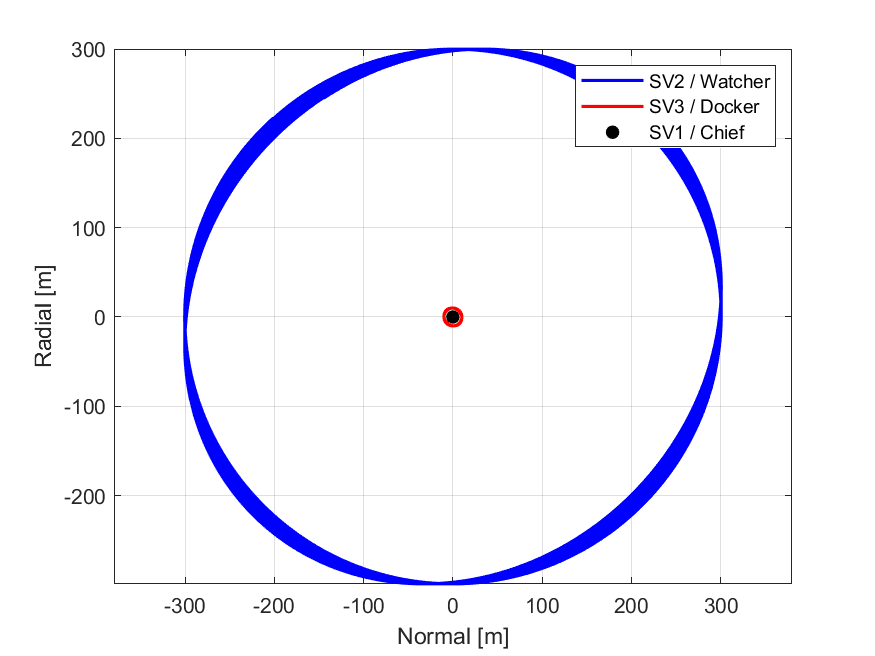
\includegraphics[width=\linewidth]{sim/figures/PS5/mode_3_RTN.png_RN.png}
        \caption{RN Projection}
        \label{fig:mode_3_rn}
    \end{subfigure}
    \begin{subfigure}[b]{0.32\linewidth}
        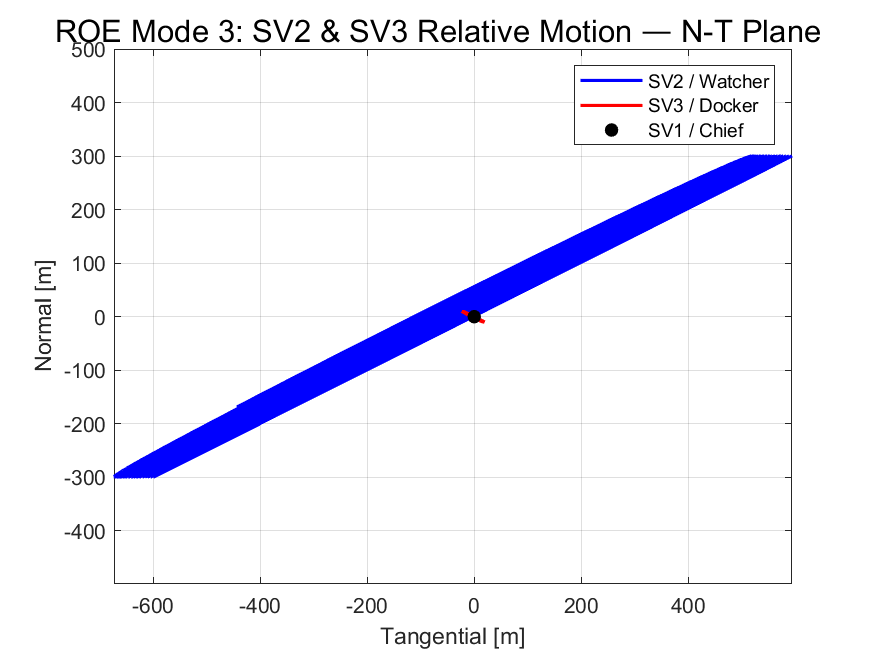
\includegraphics[width=\linewidth]{sim/figures/PS5/mode_3_RTN.png_NT.png}
        \caption{NT Projection}
        \label{fig:mode_3_nt}
    \end{subfigure}
    \caption{Mode 3 RTN Projections}
    \label{fig:mode_3_rtn}
\end{figure}

To verify that the STM is an acceptable model, it is compared in the ROE representation. As seen in Figures \ref{fig:roe_plane_compare_method} and \ref{fig:roe_time_compare_method} the STM aligns closely with the ground-truth Differences in FODE (Dif. FODE) method. The one notable exception is in the $\delta i_y$ case, although the error is very minimal.

\begin{figure}[H]
    \centering
    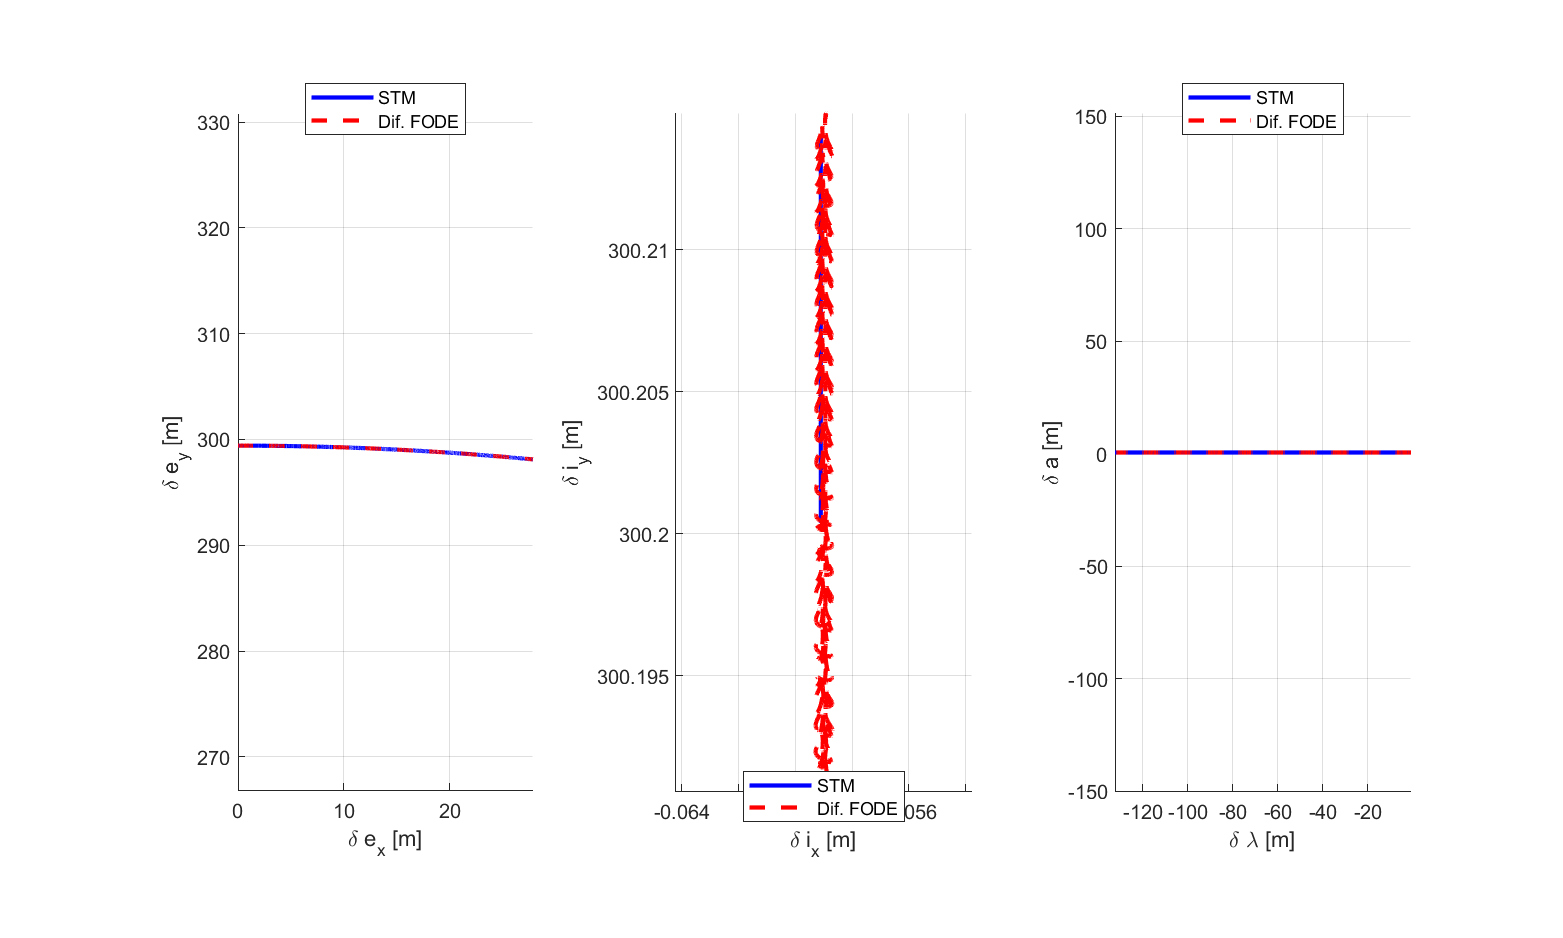
\includegraphics[width=0.75\linewidth]{sim/figures/PS5/mode_1_ROE_Planes.png}
    \caption{STM and Dif. FODE methods plotted in ROE planes}
    \label{fig:roe_plane_compare_method}
\end{figure}
\begin{figure}[H]
    \centering
    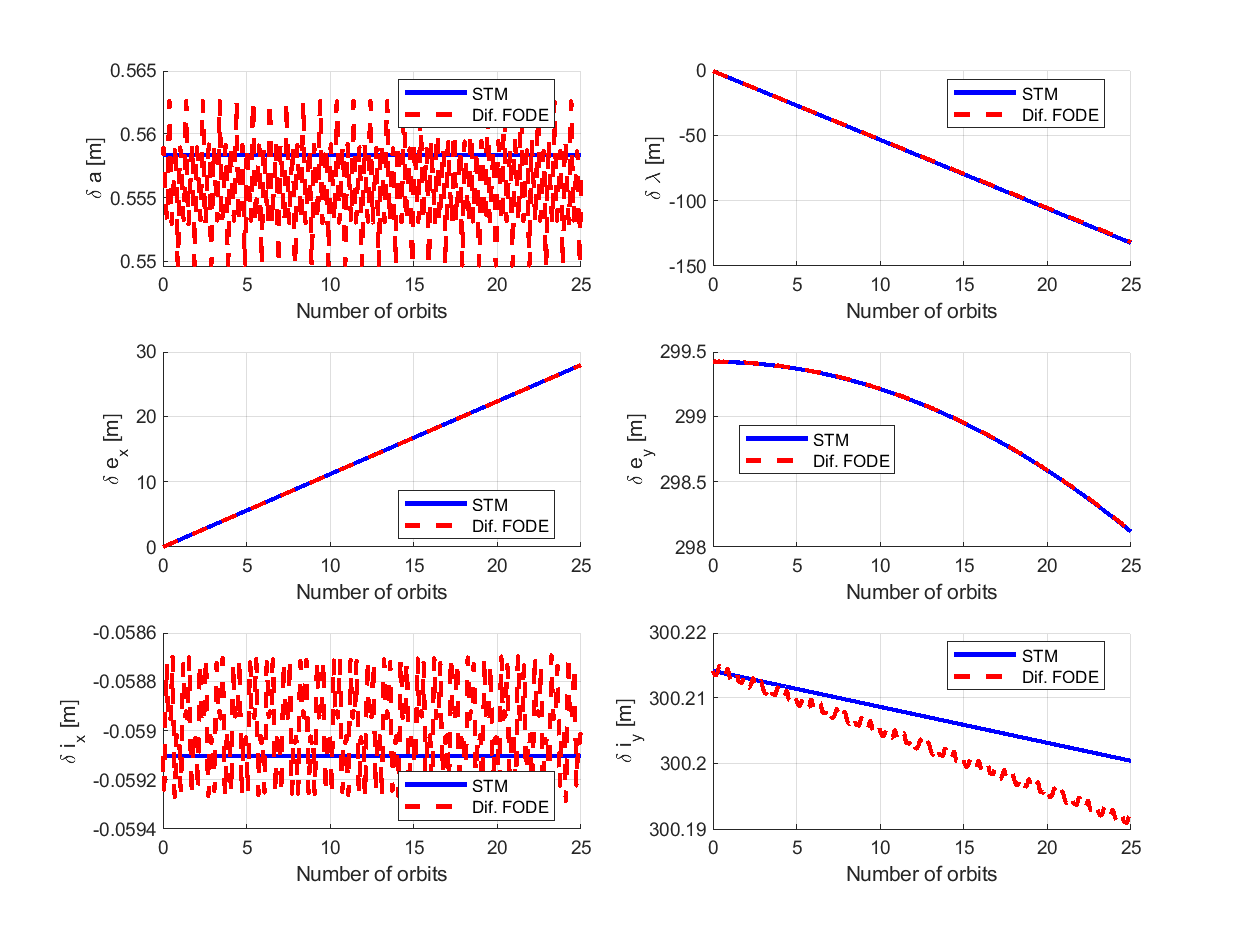
\includegraphics[width=0.75\linewidth]{sim/figures/PS5/mode_1_ROE_Time.png}
    \caption{STM and Dif. FODE methods plotted in ROE time history}
    \label{fig:roe_time_compare_method}
\end{figure}
\subsection{Impulsive Control Law}

\subsubsection{Control Method Considerations}\label{sec:control_considerations}

As highlighted in Section \ref{sec:control_objectives}, our system has four distinct operational modes, each with their own unique control accuracy and safety requirements. We also have control considerations for the maneuvers for transitioning between different modes.

Based on the requirements detailed in the previous section, we decided on the operational methods highlighted in Table \ref{tab:mode_control_methods}. Note here, that just the Docker (SV3) that performs the approach towards SV1, and so its control schemes change with time. SV2, on the other hand, keeps its original station through all modes, and does not perform any larger maneuvers (attitude maneuvers are not considered in this formulation).

\definecolor{lightgray}{gray}{0.9}

\begin{table}[H]
    \centering
    \caption{Control Methods by Mode of Operation}
    \renewcommand{\arraystretch}{1.3}

    \begin{tabularx}{\textwidth}{|>{\raggedright\arraybackslash}p{0.13\textwidth}|%
                                      >{\raggedright\arraybackslash}p{0.13\textwidth}|%
                                      >{\raggedright\arraybackslash}p{0.12\textwidth}|%
                                      >{\raggedright\arraybackslash}p{0.12\textwidth}|%
                                      >{\raggedright\arraybackslash}p{0.12\textwidth}|%
                                      >{\raggedright\arraybackslash}X|}
        \rowcolor{lightgray}
        \hline
        \textbf{Mode of Operation} & \textbf{Tracked State} & \textbf{In-plane Control Method} & \textbf{Out-of-plane Control Method} & \textbf{Control Window} & \textbf{Reasoning} \\
        \hline
        General Station Keeping (SV2 always and SV3 Mode 1) & Relative orbital elements that provide passive safety & Pairs of along-track burns & Single impulse cross-track burn & Full duration of station-keeping (see Table \ref{tab:mode_durations}) & Simple efficient control methodology that does not require prior time allocation. \\
        \hline
        Approach Transfer (SV3 Mode 2) & Desired Mode 2 final ROE & Naive least squares control solution & Naive least squares control solution & Two orbits for transfer & Simple open-loop solution, merges in-plane and out-of-plane, no drift in $\delta \lambda$ \\
        \hline
        Proximity Maneuvers (SV3 Mode 3) & Desired Mode 3 final ROE & Radial impulse burns & Single-impulse cross-track burn & Two orbits for transfer & Provides tight control, no plume on target satellite. \\
        \hline
        Docked Station Keeping (SV3 Mode 4) & N/A (Docked State) & No in-plane control & No out-of-plane control & Service duration & Rigid-body docking eliminates relative motion; no active control required. \\
        \hline
    \end{tabularx}
    \label{tab:mode_control_methods}
\end{table}



\subsubsection{Control Maneuver Formulations}



Although we had the different ideas for control methodologies for the different modes, during the duration of this submission we were only able to get one method working exactly to meet our requirements: naive least squares. Two other methods were attempted: the relative orbit control impulse burn formulations in \cite{damicothesis}, and the closed-form control solution highlighted in \cite{chernick2021optimal}. However, the method from \cite{damicothesis} causes a drift in the $\delta \lambda$ that we were not able to close (likely with a third burn). We were also unable to complete a working implementation of the closed-form solution. Although these will be discussed in later submissions (to cover all the methods detailed in Table \ref{tab:mode_control_methods}), here we will primarily discuss the naive-least squares method.

\textit{\textbf{Naive Least-Squares Method}}\\
The naive least-squares method works on the principle that a sequence of relative orbital elements can be related to each other with a linearized model that accounts for J2 perturbations, called a state transition matrix. This STM was previously stated in Equations \ref{eq:stm_matrix} and \ref{eq:state_transition_relation}. 

The change in relative orbital elements $\Delta \delta \alpha$ can also be related to the applied $\Delta v$ as \cite{chernick2021optimal}
\begin{align}
    \boldsymbol{\Delta \delta \alpha} = \Gamma\Delta \boldsymbol{v}
\end{align} \label{eq:delta_v_to_alpha}
Putting these together, we have a formulation for a set of control maneuvers $\Delta v$ required to achieve a desired change in relative orbital elements.
\begin{align}
\Delta \delta \boldsymbol{\alpha} = \delta \boldsymbol{\alpha}(t_f) - \Phi_{f,0} \, \delta \boldsymbol{\alpha}(t_0)
= \sum_{k = 1}^{M} \Phi(t_k) \Gamma (t_k)  \delta \mathbf{v}_k 
\end{align} \label{eq:delta_v_to_delta_alpha}
From theoretical formulations, we adopt the standard of setting three equally-spaced in time $\Delta v$ impulses for in-plane maneuvers, or a single impulse burn $\Delta v$ for out-of-plane maneuvers.
For near-circular orbit, the transformation matrix $\Gamma$ is given simply by
\begin{align}
\Delta \delta \boldsymbol{\alpha}_k = \Gamma_k \delta \mathbf{v}_k = \frac{1}{na}
\begin{bmatrix}
0 & 2 & 0 \\
-2 & 0 & 0 \\
\sin(u_k) & 2\cos(u_k) & 0 \\
-\cos(u_k) & 2\sin(u_k) & 0 \\
0 & 0 & \cos(u_k) \\
0 & 0 & \sin(u_k)
\end{bmatrix}
\begin{bmatrix}
\delta v_R \\
\delta v_T \\
\delta v_N
\end{bmatrix}
\end{align}

where $\Delta v$ is in the RTN frame, and $a$ is the semi-major axis of the chief SV1. We can also relate the mean argument of latitude to the maneuver time using the formulation

\begin{align}
    u_k = t_{k} \left( n + \kappa \left( \eta P + Q \right) \right) + u_{0}
\end{align}

where $P, Q, \eta, \kappa$ are defined in Equation \ref{eq:stm_matrix}.

The control maneuvers are solved by applying least-squares the linear system $M\delta v = \delta a$ which is formed by stacking all the states in the summation of Equation \ref{eq:delta_v_to_delta_alpha}.

\begin{equation}
\left[
\Phi_1 \mathbf{\Gamma}_1 \quad
\Phi_2 \mathbf{\Gamma}_2 \quad
\cdots \quad
\Phi_N \mathbf{\Gamma}_N
\right]
\begin{bmatrix}
\delta \mathbf{v}_1 \\
\delta \mathbf{v}_2 \\
\vdots \\
\delta \mathbf{v}_N
\end{bmatrix}
= M_{[6,3N]} \delta \mathbf{v}_{[3N,1]} = \Delta \delta \boldsymbol{\alpha}
\end{equation}

Using a pseudo-inverse for an analytical least-squares solution 

\begin{align}
    \delta \mathbf{v} = M^\top (M M^\top)^{-1} \Delta \delta \boldsymbol{\alpha}
\end{align}

This is our control solution, and is applied in the FODE simulation described in the following section.

\textbf{\textit{Setup Formulation}} \\
The setup of the formation reconfigurations and what we want to solve are highlighted in Section \ref{sec:control_objectives}.

\textbf{\textit{Comparing delta-v}} \\
The comparison of the least-squares method with the lower-bound delta-v $\Delta v_{lb}$ is provided in Table \ref{tab:dv_comparison}.

\textbf{\textit{Station-Keeping Maneuvers}}

Station keeping has not been fully integrated with the rest of the maneuvers yet, however we have a separate demo where we apply station keeping to prevent a drift in the relative orbital elements.
\begin{figure}[H]
    \centering
    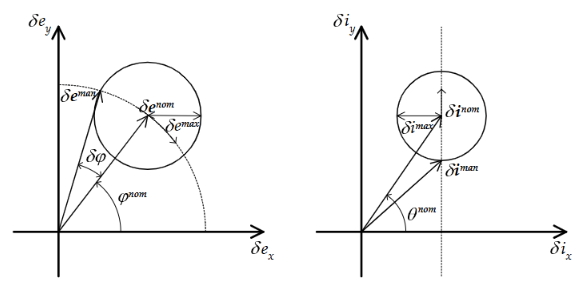
\includegraphics[width=0.75\linewidth]{sim//figures//PS5/station_keeping_man_damico.png}
    \caption{Station keeping the relative eccentricity and inclination vectors \cite{damicothesis}}
    \label{fig:station_keeping_guide}
\end{figure}

Based on Figure \ref{fig:station_keeping_guide}, we calculate the required relative orbital elements $\delta e_{man}$ and $\delta i_{man}$ that put us on the other end of the safety window. The safety window is determined by the control requirements and Equation \ref{eqn:roe_spacing}.

\subsubsection{Justificiation and Implementation of Control}

\textbf{\textit{Dynamics Model for Ground Truth Simulation}}

For our ground-truth simulation model, we utilized a FODE simulation model that is described in Section \ref{sec:fode_simulation}. This model gives us a high-fidelity model in which it is simple to incorporate J2 perturbations and drag models (although the drag models have not been implemented yet). The states of the satellites are stored and propagated in ECI co-ordinates. 

When simulating a maneuver, the propagation is stopped, the required $\delta v$ is added to the state, and then the propagation is continued. This allows us to simulate the impulsive burns. The $\delta v$ burns, which are calculated in RTN frame as a result of the naive least-squares and converted to ECI based on the chief's state at maneuver time.

Separate from the primary simulation that implemented the different modes and maneuvers, we implemented a more integrated simulation for station-keeping that continuously plans maneuvers if the eccentricity vector or inclination vector go beyond the safe region. The code structure for station keeping, which will also simulate the primary larger maneuvers in the future, is shown in Algorithm \ref{alg:station_keeping}.

\begin{algorithm}[H]
\caption{Station=keeping Simulation and Plotting}
\begin{algorithmic}[1]

\State Initialize time array, chief semi-major axis, and empty state histories
\State Extract nominal ROE for SV2 and SV3
\State Define station-keeping bounds
\State Compute desired eccentricity offsets

\For{each time step $t_i$ in $t_{\text{series}}$}
    \State Propagate SV1, SV2, SV3 states using RK4
    \State Convert SV2 and SV3 states to ROE w.r.t. SV1

    \If{SV has not yet performed control}
        \If{eccentricity deviation exceeds threshold}
            \State Compute station keeping maneuver with naive least squares (3 burns)
            \State Store SV $\Delta v$ for eccentricity control
        \EndIf
        \If{inclination deviation exceeds threshold}
            \State Compute station keeping maneuver with naive least squares (1 burn)
            \State Store SV $\Delta v$ for inclination control
        \EndIf
    \EndIf
    \If{a planned SV $\Delta v$ is scheduled now}
        \State Apply $\Delta v$ to SV and remove it from queue
    \EndIf
\EndFor

\State Convert SV2 and SV3 final states to RTN position relative to SV1\EndProcedure
\end{algorithmic}
\end{algorithm} \label{alg:station_keeping}

\textbf{\textit{Selection of Dynamics Model for Controller}} \\
The naive least-squares utilizes the STM for near-circular orbits detailed in Equation \ref{eq:stm_matrix} to propagate the state. Control maneuvers calculate $\delta v$ in the RTN frame, the input and reference ROEs use quasi-nonsingular relative orbital elements.

\textbf{\textit{Actuator Implementation, Sensor and Disturbance Models}} \\
For this submission, considerations of the delta-v budget, actuator implementation, sensor models, and disturbance models (apart from J2) are ignored. These other practical considerations will be incorporated in future submissions.

\subsubsection{Results and Analysis of Control Performance} \label{sec:analysis_of_control}

The results of the control system are shown in the following figures. Note that these figures do not include station-keeping control in between the modes, as this will be implemented in the future. This is why there are still significant drifts in the station keeping modes from J2. 

Figures \ref{fig:roe_planes_modes} and \ref{fig:roe_time_modes} show the desired and actual ROEs for each mode. $\delta a$ becomes non-zero during the maneuvers because there are along-track elements. However, at the end of each mode, the control system is able to reduce $\delta a$ to near zero. But due to $\delta a$ and $\delta i_x$ not being precisely zero throughout the control and station-keeping modes, a drift is introduced in $\delta \lambda$. $\delta e_x$ and $\delta i_x$ are always meant to be zero, but again the maneuvers introduce variations. Each control mode tries to return $\delta e_x$ and $\delta i_x$ to zero but is unable to get all the way there. These errors can be addressed by station-keeping control in between modes. $\delta e_y$ and $\delta i_y$ exhibit the most accurate behavior. The control system is able to reach the desired $\delta e_y$ and $\delta i_y$ in each mode with very little error. This is important because these are the only non-zero factors in the desired ROEs and drive passive safety. 

\begin{figure}[H]
    \centering
    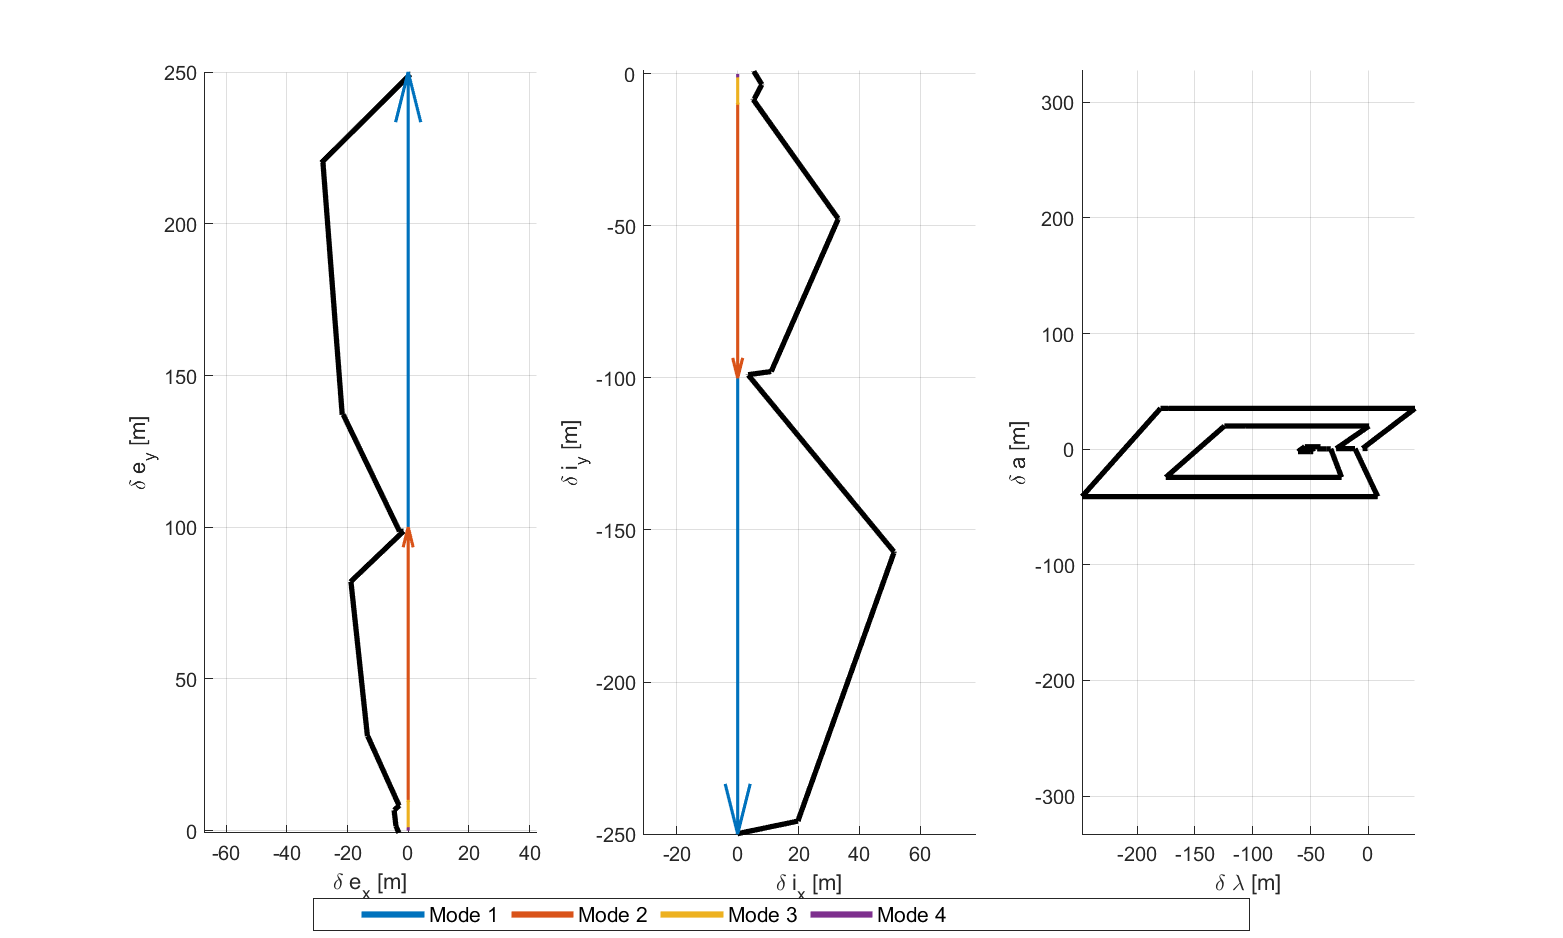
\includegraphics[width=0.75\linewidth]{sim/figures/PS5/ROE_planes_modes.png}
    \caption{Actual and desired ROE plotted for all modes in ROE planes}
    \label{fig:roe_planes_modes}
\end{figure}
\begin{figure}[H]
    \centering
    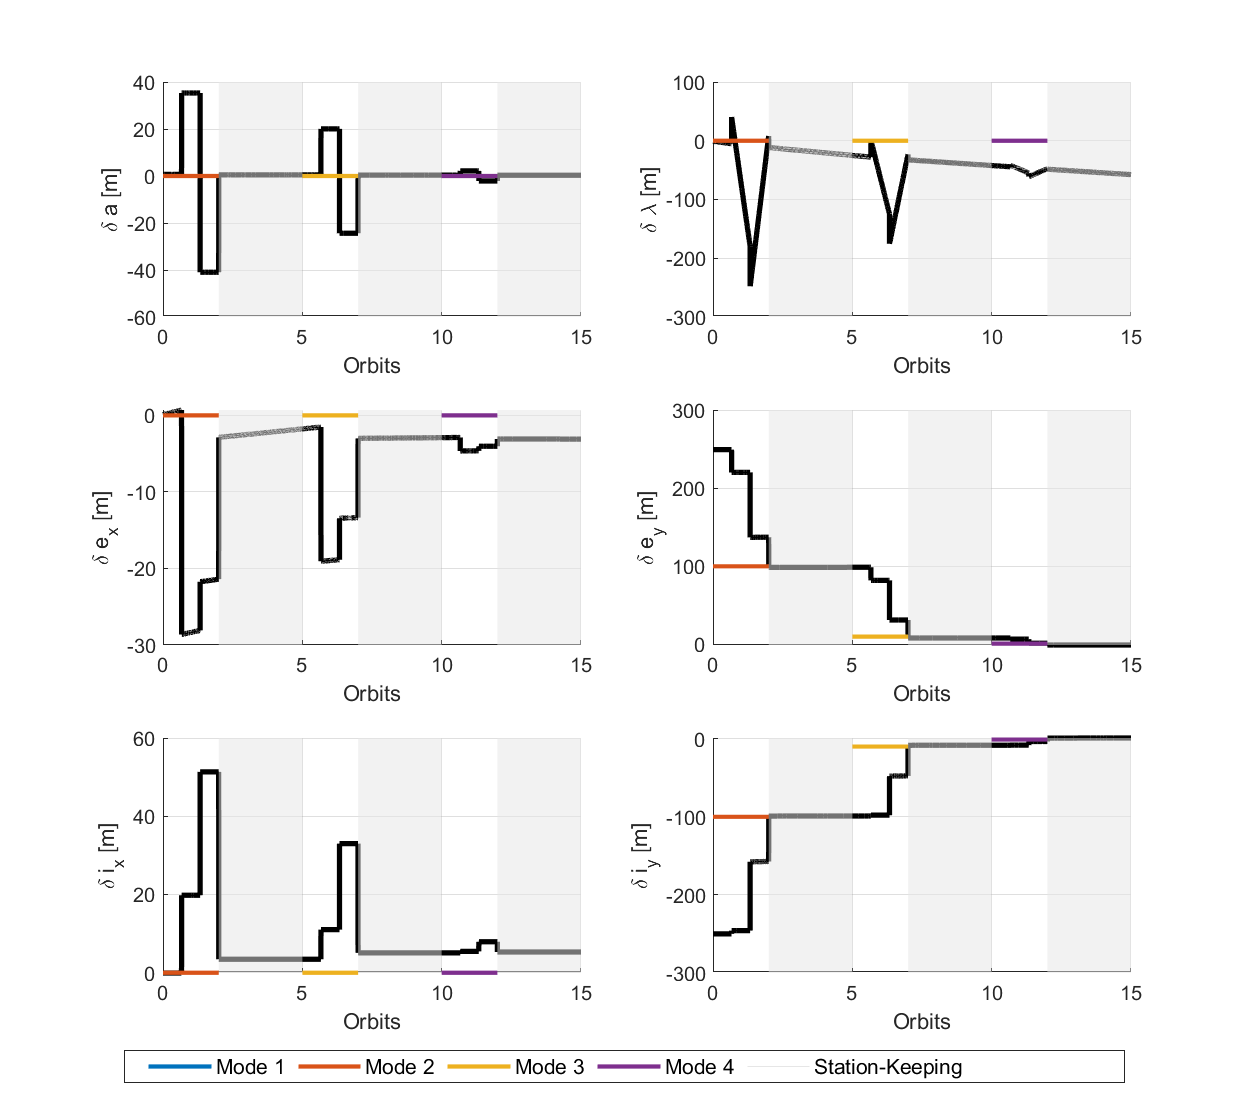
\includegraphics[width=0.75\linewidth]{sim/figures/PS5/ROE_over_time_modes.png}
    \caption{Actual and desired ROE plotted for all modes in ROE time history}
    \label{fig:roe_time_modes}
\end{figure}

Figure \ref{fig:roe_error_time_modes} reflects the same behavior in the tracking errors. The control system is able to track $\delta a, \delta e_y, and \delta i_y$ very well. The other tracking errors can be corrected either through station-keeping control or the usage of another control method. The naive least-squares method produces delta-v's that are in all directions in RTN. Other closed-form approaches, such as reachable set theory are able to specify more precise maneuvers that do not have as many unwanted side effects on other ROEs. 

\begin{figure}[H]
    \centering
    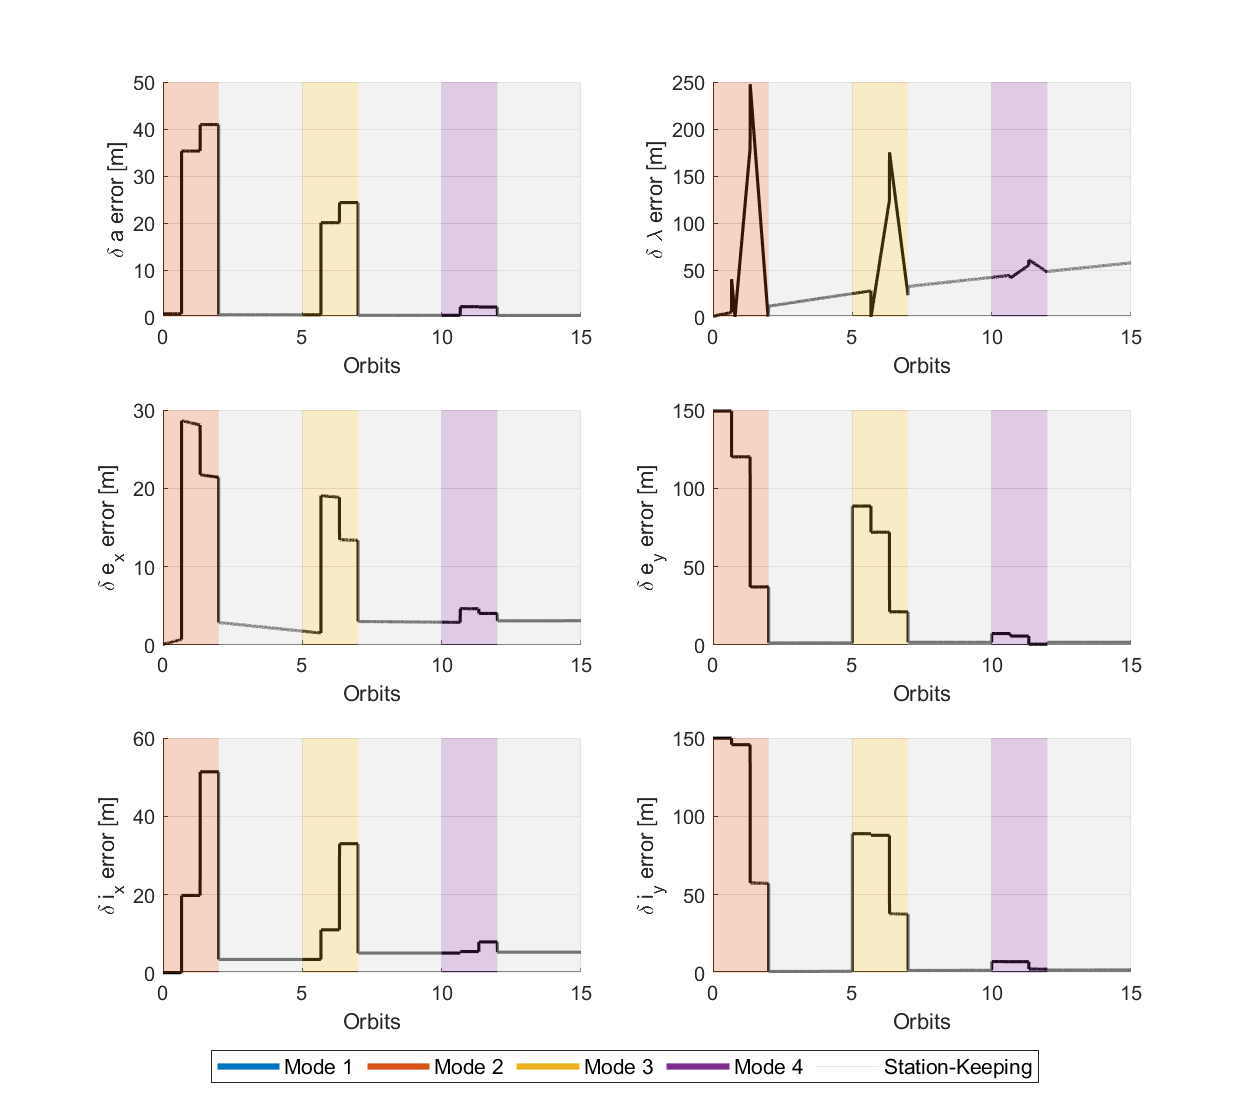
\includegraphics[width=0.75\linewidth]{sim/figures/PS5/ROE_error_over_time_modes.png}
    \caption{Tracking error between actual and desired ROE plotted for all modes in ROE time history}
    \label{fig:roe_error_time_modes}
\end{figure}

Figure \ref{fig:delta_v_modes} shows the delta-v magnitudes in the RTN directions throughout each control mode. As expected, delta-v magnitudes are on the order of mm/s. The magnitudes decrease in size as the desired change in ROE decreases throughout the modes. Additionally, the magnitudes in the normal direction are multiple times larger than those in radial or tangential. This arises from the fact that inclination maneuvers are much more expensive than eccentricity maneuvers. Since each mode changes relative eccentricity and relative inclination by the exact same magnitude, the inclination maneuver is going to have to be larger. 
\begin{figure}[H]
    \centering
    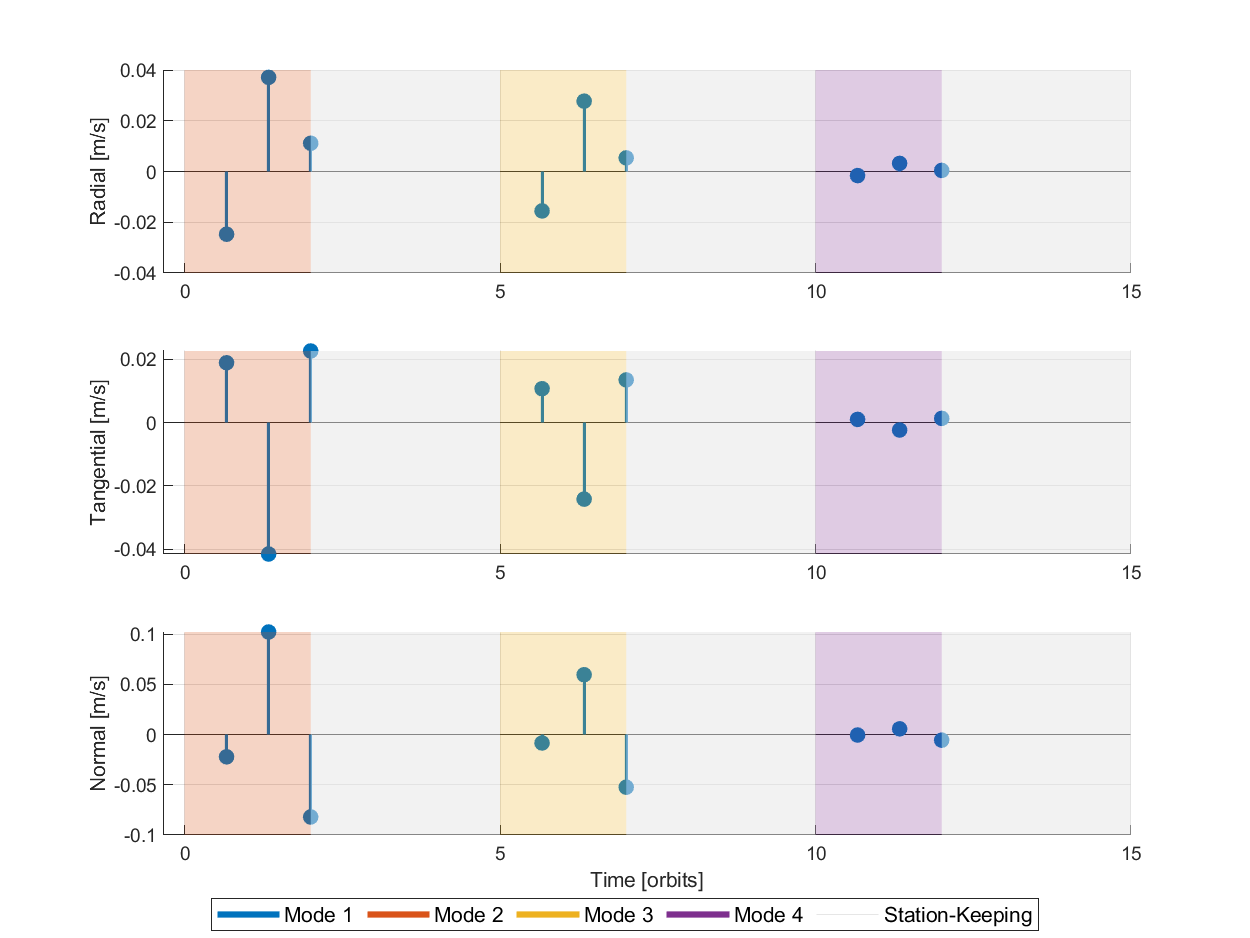
\includegraphics[width=0.75\linewidth]{sim/figures/PS5/delta_v_timeline_modes.png}
    \caption{Actual delta-v of control maneuvers over time}
    \label{fig:delta_v_modes}
\end{figure}

As a point of comparison, the theoretical delta-v lower bound can be calculated as follows:
\begin{align*}
\Delta v_{\text{ecc}} &= \frac{1}{2} \cdot n \cdot a \cdot \left\| \Delta \delta\vec{e} \right\| \\
\Delta v_{\text{inc}} &= n \cdot a \cdot \left\| \Delta \delta\vec{i} \right\| \\
\Delta v_{\text{lb}} &= \sqrt{\Delta v_{\text{ecc}}^2 + \Delta v_{\text{inc}}^2}
\end{align*}
Note that only changes in ROEs were in $\delta e$ and $\delta i$, which is why delta-v lower bound can be calculated as the norm of the along-track and cross-track delta-v's. 

Table \ref{tab:dv_comparison} compares the total delta-v with the theoretical lower-bound. The actual delta-v's were approximately double the theoretical lower-bound for each mode. This suggests that there is room for improvement in optimizing the delta-v cost, which methods like reachable set theory could offer. 
\begin{table}[h!]
\centering
\begin{tabular}{|c|c|c|}
\hline
\textbf{Mode} & \textbf{Total }$\Delta v$ \textbf{(m/s)} & \textbf{Lower Bound (m/s)} \\
\hline
2 & 0.3624 & 0.1830 \\
3 & 0.2174 & 0.1098 \\
4 & 0.0216 & 0.0110 \\
\hline
\end{tabular}
\caption{Total delta-$v$ compared with theoretical lower bounds for each maneuver mode}
\label{tab:dv_comparison}
\end{table}

As mentioned previously, the station-keeping mode was treated separately to the other modes for the time being. The algorithm for station keeping is provided in Algorithm \ref{alg:station_keeping}. Ultimately, the station-keeping mode will be integrated into the full control system to prevent drift in ROEs when maintaining a formation. Figures \ref{fig:roe_planes_stk} and \ref{fig:roe_time_stk} show the current performance of the station-keeping control method. While there is still some erroneous behaviors, the control method successfully prevents drift in $\delta \lambda$ which is key for our formation to stay centered around the Target. The keep-in zone was set to a 1-meter radius circle centered on the desired ROEs. The control method is generally able to keep errors to below 5 meters. In future work, the unexpected behavior towards the end of the time series will be addressed. Also, the keep-in zone of 1 meter might be too tight for the current formulation, leading to this undesired behavior. 

\begin{figure}[H]
    \centering
    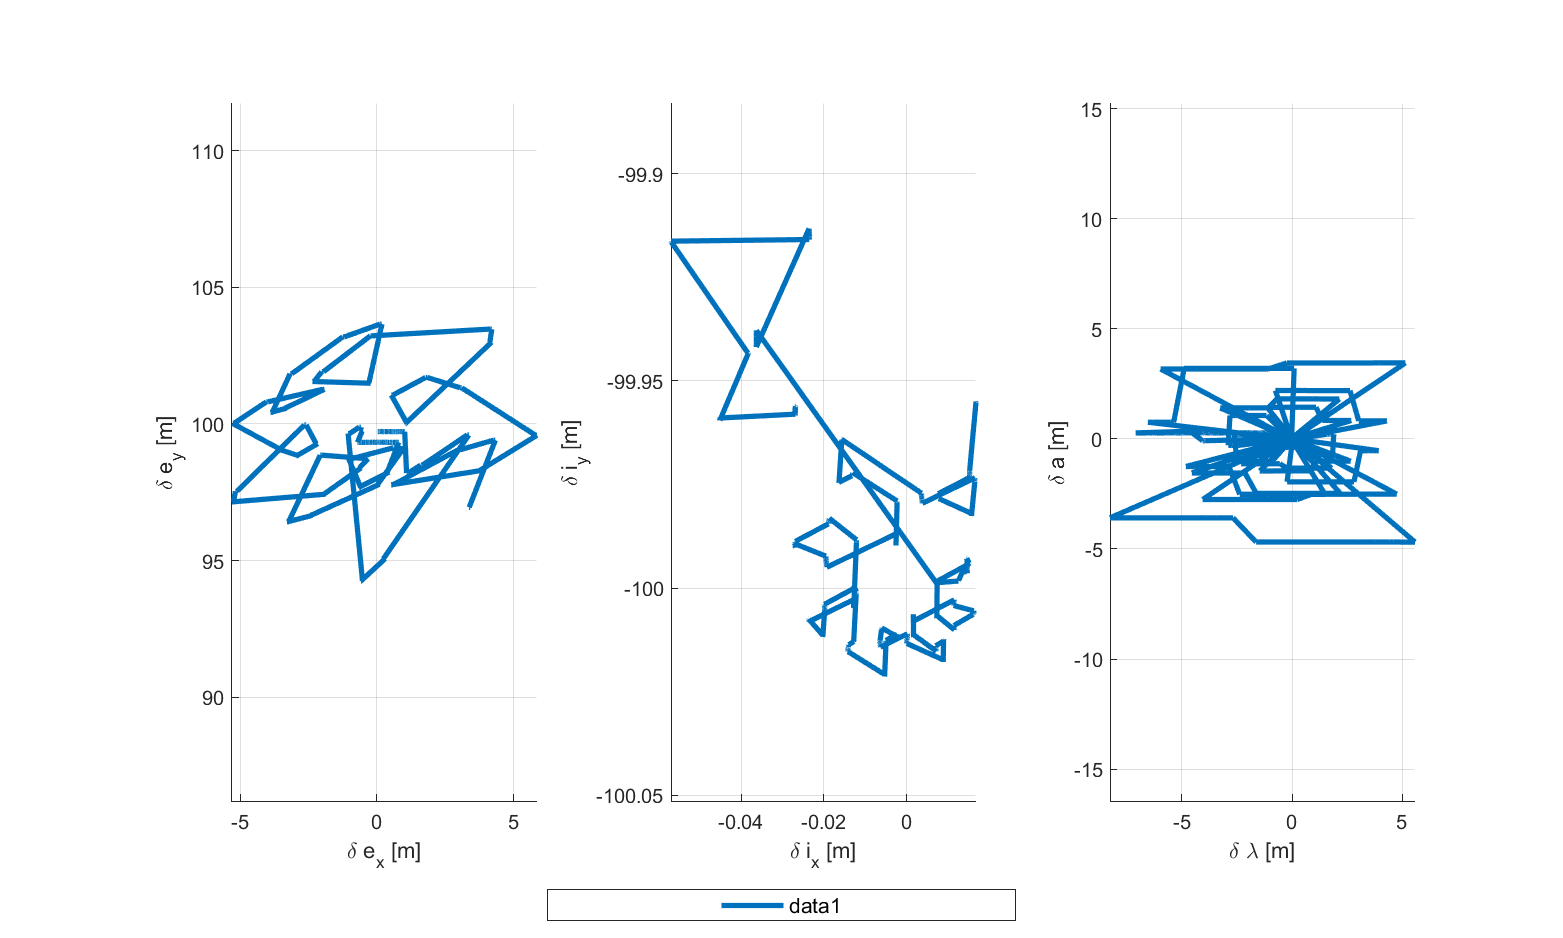
\includegraphics[width=0.7\linewidth]{sim/figures/PS5/ROE_planes.png}
    \caption{Station-keeping mode in ROE planes}
    \label{fig:roe_planes_stk}
\end{figure}

\begin{figure}[H]
    \centering
    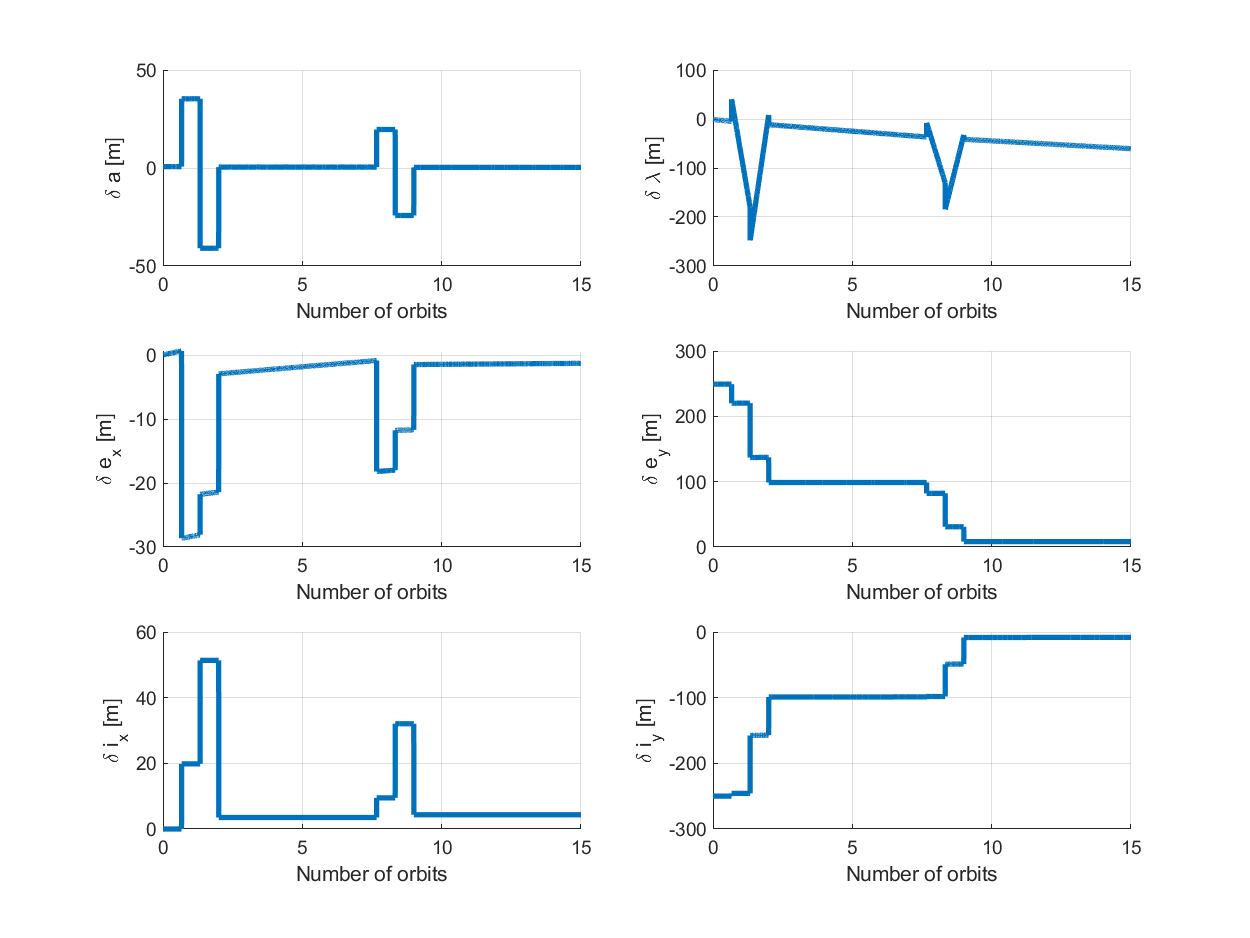
\includegraphics[width=0.7\linewidth]{sim/figures/PS5/ROE_over_time.png}
    \caption{Station-keeping mode in ROE time history}
    \label{fig:roe_time_stk}
\end{figure}


\newpage
\section{Problem Set 6}

\subsection{Continuous Control Law}

\subsubsection{Control Method Considerations}

The control method considerations are the same as in Section \ref{sec:control_objectives} and Section \ref{sec:control_considerations}. Our system has four distinct operational modes, each with their own unique control accuracy and safety requirements. We also have control considerations for the maneuvers for transitioning between different modes. In this section, we utilize a continuous control input rather than impulse delta-v inputs.

To provide enough time for the continuous control to act effectively, we increased the duration of each mode (maneuver times and station keeping times between maneuvers), provided in Table \ref{tab:mode_durations_cont}.

\begin{table}[h!]
\centering
\begin{tabular}{|c|c|}
\hline
\textbf{Phase} & \textbf{Number of Orbits} \\
\hline
Mode 2 & 15 \\
Station-Keeping 2 & 5 \\
Mode 3 & 10 \\
Station-Keeping 3 & 5 \\
Mode 4 & 10 \\
Station Keeping 4 & 5 \\
\hline
\end{tabular}
\caption{Number of orbits spent in each mode and station-keeping phase} \label{tab:mode_durations_cont}
\end{table}

Our system is still working in a near-circular orbit with two deputy spacecraft. The "Watcher/SV2" spacecraft only performs station-keeping, whereas the "Docker/SV3" performs various maneuvers to dock with the chief spacecraft. Table \ref{tab:mode_control_methods_cont} is analogous to Table \ref{tab:mode_control_methods}, but with continuous control methods considered.


\definecolor{lightgray}{gray}{0.9}

\begin{table}[H]
    \centering
    \caption{Control Methods by Mode of Operation}
    \renewcommand{\arraystretch}{1.3}

    \begin{tabularx}{\textwidth}{|>{\raggedright\arraybackslash}p{0.13\textwidth}|%
                                      >{\raggedright\arraybackslash}p{0.13\textwidth}|%
                                      >{\raggedright\arraybackslash}p{0.12\textwidth}|%
                                      >{\raggedright\arraybackslash}p{0.12\textwidth}|%
                                      >{\raggedright\arraybackslash}p{0.12\textwidth}|%
                                      >{\raggedright\arraybackslash}X|}
        \rowcolor{lightgray}
        \hline
        \textbf{Mode of Operation} & \textbf{Tracked State} & \textbf{In-plane Control Method} & \textbf{Out-of-plane Control Method} & \textbf{Control Window} & \textbf{Reasoning} \\
        \hline
        General Station Keeping (SV2 always and SV3 Mode 1) & Relative orbital elements that provide passive safety & Along-track continuous control input & Cross-track continuous control input & Full duration of station-keeping (see Table \ref{tab:mode_durations}) & Very small control inputs to maintain position when needed. \\
        \hline
        Approach Transfer (SV3 Mode 2) & Desired Mode 2 final ROE & Along-track continuous control input & Cross-track continuous control input & 15 orbits for maneuver & Using Lyapunov-based control scheme with modifications for handling $\delta \lambda $ drift\\
        \hline
        Proximity Maneuvers (SV3 Mode 3) & Desired Mode 3 final ROE & Along-track continuous control input & Cross-track continuous control input & 15 orbits for maneuver & Using Lyapunov-based control scheme with modifications for handling $\delta \lambda $ drift\\
        \hline
        Docked Station Keeping (SV3 Mode 4) & N/A (Docked State) & No in-plane control & No out-of-plane control & Service duration & Rigid-body docking eliminates relative motion; no active control required. \\
        \hline
    \end{tabularx}
    \label{tab:mode_control_methods_cont}
\end{table}


\subsubsection{Lyapunov Control Implementation}\label{sec:Lyapunov_implementation}
Although we had the different ideas for control methodologies for the different modes, during the duration of this submission we were only able to get one method working exactly to meet our requirements: Lyapunov control without constraints. 

First, the state-space reduced model as described by Steindorf is considered \cite{steindorf2017constrained}. Since tangential thrusts are two times more efficient than radial thrusts in changing $\delta e$ and $\delta a$, the reduced model does not involve any radial thrusts. Thus, the ROE vector is reduced to exclude $\delta \lambda$, since it can only be controlled directly by radial thrusts.Note that $\delta \lambda$ can still be controlled by adjusting $\delta a$ to induce a Keplerian drift such that $\delta \lambda$ reaches a desired state at the end of the control window. This process will be desribed in full later. The reduced ROE vector is defined as: 
\begin{align*}
\delta \bm{\alpha} = \begin{bmatrix} \delta a, \delta e_x, \delta e_y, \delta i_x, \delta i_y \end{bmatrix}^\top
\end{align*}

From here the reduced state-space model can be defined as follows:
\begin{equation}
\begin{bmatrix}
\delta \dot{\bm{\alpha}} \\
\delta \ddot{a}
\end{bmatrix}
=
A
\begin{bmatrix}
\delta \bm{\alpha} \\
\delta \dot{a}
\end{bmatrix}
+
\begin{bmatrix}
B \\
\bm{0}_{1 \times 3}
\end{bmatrix}
\bm{u}
\label{eq:reduced_state_space}
\end{equation}

The reduced ROE state is augmented by the differential rate of change of the relative semi-major-axis, $\delta \dot{a}$. This is to  deal with aerodynamic drag, but that is neglected in our case. 

The plant matrix for the reduced model with J2 effects is given by:
\begin{equation}
A_{J2}(\bm{\alpha}_c) = \kappa
\begin{bmatrix}
0 & 0 & \frac{7}{2} e_y Q & -4 e_x e_y G Q & -(1 + 4 e_y^2 G) Q & 5 e_y S & 0 & 0 \\
0 & 0 & -\frac{7}{2} e_x Q & (1 + 4 e_x^2 G) Q & 4 e_x e_y G Q & -5 e_x S & 0 & 0 \\
0 & 0 & 0 & 0 & 0 & 0 & 0 & 0 \\
0 & 0 & \frac{7}{2} S & -4 e_x G S & -4 e_y G S & 2 T & 0 & 0 \\
0 & 0 & 0 & 0 & 0 & 0 & 0 & 0 \\
\end{bmatrix}
\end{equation} \label{eq:continuous_control_A}
\noindent where
\[
\dot{\omega} = \kappa Q; \qquad \gamma = \frac{3}{4} J_2 R_e^2 \sqrt{\mu}; \qquad \eta = \sqrt{1 - e^2}; \qquad \kappa = \frac{\gamma}{a_c^{7/2} \eta_c^4}
\]

\[
e_x = e_c \cos(\omega_c); \qquad e_y = e_c \sin(\omega_c); \qquad E = 1 + \eta_c; \qquad F = 4 + 3 \eta_c; \qquad G = \frac{1}{\eta_c^2}
\]

\[
P = 3 \cos(i_c)^2 - 1; \qquad Q = 5 \cos(i_c)^2 - 1; \qquad S = \sin(2 i_c); \qquad T = \sin(i_c)^2
\]

The control input matrix for the reduced model is given by:

\begin{equation}
\bm{B}(\bm{\alpha}_c) = \frac{1}{a n}
\begin{bmatrix}
\frac{2}{\eta}(1 + e \cos f) & 0 \\
\eta \frac{(2 + e \cos f) \cos \theta + e_x}{1 + e \cos f} & \frac{\eta e_y}{\tan i} \cdot \frac{\sin \theta}{1 + e \cos f} \\
\eta \frac{(2 + e \cos f) \sin \theta + e_y}{1 + e \cos f} & -\frac{\eta e_x}{\tan i} \cdot \frac{\sin \theta}{1 + e \cos f} \\
0 & \eta \frac{\cos \theta}{1 + e \cos f} \\
0 & \eta \frac{\sin \theta}{1 + e \cos f}
\end{bmatrix}
\end{equation} \label{eq:continuous_control_B}

where \( f \) is the true anomaly and \( \theta = f + \omega \).

And the control input is given by:
\begin{equation}
\bm{u} = \begin{bmatrix} u_t, u_n \end{bmatrix}^\top
\end{equation}
which represents the control acceleration in along-track and normal directions of the co-rotating RTN frame.

For continuous control, a feedback controller can be implemented to stabilize the system at a desired reference, $\delta \boldsymbol{\alpha}_a$. A control law that ensures the relative state to asymptotically tend towards the desired reference is given by: 

\begin{equation}
\mathbf{u} = -\mathbf{B}^* \left[ A \delta \boldsymbol{\alpha} + P \left( \delta \boldsymbol{\alpha} - \delta \boldsymbol{\alpha}_a \right) \right]
\label{eq:feedback_continuous}
\end{equation}

To ensure that this control law achieves asymptotic stability, a Lyapunov function which is positive definite and whose time derivative is negative definite is chosen. Let the reduced state-space system described by Equation \ref{eq:reduced_state_space} be subject to the control law given in Equation \ref{eq:feedback_continuous} with $P$ being positive definite. A Lyapunov function candidate is given by:

\begin{equation}
V(\delta \boldsymbol{\alpha}_a, \delta \boldsymbol{\alpha}) = \frac{1}{2} (\delta \boldsymbol{\alpha} - \delta \boldsymbol{\alpha}_a)^\top (\delta \boldsymbol{\alpha} - \delta \boldsymbol{\alpha}_a) 
= \frac{1}{2} \Delta \boldsymbol{\alpha}^\top \Delta \boldsymbol{\alpha}
\label{eq:Lyapunov_candidate}
\end{equation}

By taking the derivative of Equation \ref{eq:Lyapunov_candidate} and substituting Equation \ref{eq:feedback_continuous} into Equation \ref{eq:Lyapunov_candidate}, it can be proven that Equation \ref{eq:Lyapunov_candidate} is a Lyapunov function:

\begin{align}
\dot{V}(\delta \boldsymbol{\alpha}_a, \delta \boldsymbol{\alpha}) 
&= \Delta \boldsymbol{\alpha}^\top \Delta \dot{\boldsymbol{\alpha}} \notag \\
&= \Delta \boldsymbol{\alpha}^\top \left( \dot{\delta \boldsymbol{\alpha}} - \dot{\delta \boldsymbol{\alpha}}_a \right) \notag \\
&= \Delta \boldsymbol{\alpha}^\top \left( A(\alpha_c) \delta \boldsymbol{\alpha} + B(\alpha_c) \mathbf{u} - 0 \right) \notag \\
&= \Delta \boldsymbol{\alpha}^\top \left( A(\alpha_c) \delta \boldsymbol{\alpha} + B(\alpha_c) \left( -\mathbf{B}^* \left[ A \delta \boldsymbol{\alpha} + P(\delta \boldsymbol{\alpha} - \delta \boldsymbol{\alpha}_a) \right] \right) \right) \notag \\
&= -\Delta \boldsymbol{\alpha}^\top P \Delta \boldsymbol{\alpha}
\tag{4.3}
\end{align}

which is negative definite.

The matrix \( P \) is defined as:

\[
P = \frac{1}{k} \begin{bmatrix}
\cos(J)^N & 0 & 0 & 0 & 0 \\
0 & \cos(J)^N & 0 & 0 & 0 \\
0 & 0 & \cos(J)^N & 0 & 0 \\
0 & 0 & 0 & \cos(H)^N & 0 \\
0 & 0 & 0 & 0 & \cos(H)^N \\
\end{bmatrix}
\]

where \( k \in \mathbb{R}^{+} \) is an arbitrary large scaling scalar, 
\( J = u - \bar{u}_{ip} \), \( H = u - \bar{u}_{oop} \), and 
\( u = M + \omega \) is the mean argument of latitude. 
The exponent \( N \in \mathbb{N} \) such that \( N \bmod 2 = 0 \land N > 2 \) 
defines to which extent the control inputs are centered around the fuel optimal locations to control the in-plane \((\delta a, \delta e)\) motion at \( \bar{u}_{ip} \), and the out-of-plane \((\delta i)\) motion at \( \bar{u}_{oop} \).

The optimal locations for near-circular orbits to apply thrust are given by:

\[
\bar{u}_{ip} = \text{atan2} \left( \Delta \delta e_y, \Delta \delta e_x \right)
\]
\[
\bar{u}_{oop} = \text{atan2} \left( \Delta \delta i_y, \Delta \delta i_x \right)
\]

The parameters $N$ and $k$ are used to tune the controller response. 

\textbf{\textit{Indirect Control of $\delta\lambda$}}

Direct control of $\delta \lambda$ would require the additional degree of freedom of radial burns, which can be very inefficient for $\Delta v$ usage. Instead, $\delta \lambda$ can be corrected indirectly by using along-track burns and applying an intermediate $\delta a_{des}$, and allowing for Keplerian dynamics to drift $\delta \lambda$ by a desired amount. \cite{steindorf2017constrained}

The rate of change of the $\delta \lambda$ is based on the semi-major axis separation $\delta a$
\begin{align}
    \delta \dot{\lambda} = -\frac{3}{2}n_c \delta a 
\end{align}
We can thus modulate the $\delta a_{des}$ such that we can help converge $\delta \lambda$ to zero by the end of the maneuver period. We can thus set up a desired $\delta \dot{\lambda}$ that helps converge $\Delta \delta \lambda \rightarrow 0$
\begin{equation}
\delta \dot{\lambda}_a =
\begin{cases}
-\min \left\{ \left| \frac{\Delta \delta \lambda}{\tau} \right| , \delta \dot{\lambda}_{\text{ref}} \right\}, & \text{if } \Delta \delta \lambda \geq 0 \\
\phantom{-}\min \left\{ \left| \frac{\Delta \delta \lambda}{\tau} \right| , \delta \dot{\lambda}_{\text{ref}} \right\}, & \text{if } \Delta \delta \lambda < 0
\end{cases}
\end{equation}

We determine those upper bounds $\delta \dot{\lambda}_{ref}$ based on a $\delta a_{ref}$
\begin{align}
    \delta \dot{\lambda}_{ref} = \frac{3}{2} n_c \delta a_{ref}
\end{align}

where $\delta a_{ref}$ accounts for the shift in $\delta a$ that occurs when performing tangential burns to modify the in-plane eccentricity vector change $\Delta \delta \textbf{e}$. We thus use the following expression for $\delta a_{ref}$ as
\begin{align}
    \delta a_{ref} &= \left|\frac{1}{a_cn_c \eta}(1 + e \cos(f))\cdot  \frac{v_{opt}}{2\cdot n_{orbits}}\right| \\
    v_{opt} &= \frac{a_cn_c||\Delta\delta \textbf{e}||_2}{2\eta}
\end{align}

With this, we now have all the information required to calculate $\delta \dot{\lambda}_a $, from which we can calculate the new target $\delta a_a$ that we should have the Lyapunov controller track to cause the desired shift in $\delta \lambda$.
\begin{align}
    \delta a_a = -\frac{2}{3}\frac{\delta \dot{\lambda}_a}{n_c}
\end{align}
This is then utilized as an intermediary reference $\delta a$. The new $\Delta \delta a = \delta a - \delta a_a$, rather than using a reference of $\delta a_a = 0$.

There is an additional accomodation made to the matrix P to bound the maximum tracking error to be around $\delta a_{ref}$, to prevent the tracking error from increasing to an amount that then conflicts with the control burn required for eccentricity vector correction. The adjustment to matrix P is just setting terms to $0$ to stop feedback of any tracking error that gets larger than $\delta a_{ref}$.

\[
P_{|\delta a_a| \geq |\delta a_{ref}|} = \frac{1}{k} \begin{bmatrix}
0 & 0 & 0 & 0 & 0 \\
0 & 0 & 0 & 0 & 0 \\
0 & 0 & 0 & 0 & 0 \\
0 & 0 & 0 & \cos(H)^N & 0 \\
0 & 0 & 0 & 0 & \cos(H)^N \\
\end{bmatrix}
\]

\subsubsection{Justificiation and Implementation of Control}

\textbf{\textit{Dynamics Model for Ground Truth Simulation}}

For our ground-truth simulation model, we utilized a FODE simulation model that is described in Section \ref{sec:fode_simulation} (utilizing RK4). This model gives us a high-fidelity model in which it is simple to incorporate J2 perturbations and drag models (although the drag models have not been implemented yet). The states of the satellites are stored and propagated in ECI co-ordinates. 

Based on the time-index of the simulation, it is decided whether station-keeping or maneuevering to the specified ROEs of the next mode is required. Then, the lyapunov control scheme is utilized to calculate required acceleration control inputs in the tangential and normal directions. These are then applied as an approximate change in velocity to the ECI state vector being propagated. The full structure of this code is shown in Algorithm \ref{alg:continuous_control_sim}
\begin{align}
    \Delta v_t = u_t \Delta t
\end{align}

\begin{algorithm}[H]
\caption{FODE Simulation with Continuous Control}
\begin{algorithmic}[1]

\State Initialize time array, chief semi-major axis, and empty state histories
\State Get maneuver control block times
\State Extract nominal ROE for SV2 and SV3

\For{each time step $t_i$ in $t_{\text{series}}$}
    \State Propagate SV1, SV2, SV3 states using RK4
    \State Convert SV2 and SV3 states to ROE w.r.t. SV1

    \State Compute control input to station-keep SV2
    \If{$t_i$ belongs to a maneuver block}
        \State Get desired final ROE values for SV3
        \State Compute control input to maneuver SV3
    \Else
        \State Compute control input to station-keep SV3
    \EndIf
    \State Convert control inputs to a change in $\Delta v$ in the ECI frame
    \State Apply control input
\EndFor
\State Convert SV2 and SV3 final states to RTN position relative to SV1
\State Plot desired data in RTN and ROE frames.
\EndProcedure
\end{algorithmic}
\end{algorithm} \label{alg:continuous_control_sim}

\textbf{\textit{Selection of Dynamics Model for Continuous Controller}} \\
The Lyapunov-based control uses a reduced-order model as an approximation of the true dynamics that can be utilized for control design. This reduced order model is captured in the $A$ and $B$ matrices provided in Equation \ref{eq:continuous_control_A} and \ref{eq:continuous_control_B}. Control maneuvers calculate a control input $u_t$ in the RTN frame (which is converted to ECI when being applied to FODE states), and the input and reference ROEs use quasi-nonsingular relative orbital elements.

\textbf{\textit{Actuator Implementation, Sensor and Disturbance Models}} \\
For this submission, considerations of the delta-v budget, actuator implementation, sensor models, and disturbance models (apart from J2) are ignored. These other practical considerations will be incorporated in future submissions.

\subsubsection{Results and Analysis of Continuous Control Performance} \label{sec:analysis_of_control_cont}

The results of the Lyapunov-based unconstrained continuous control scheme are shown in the following figures. These plots include all modes of the Watcher (SV2) and Docker (SV3) satellites, which involve maneuvers between desired ROEs and station-keeping.

Figures \ref{fig:cont_control_RT}, \ref{fig:cont_control_RN}, and \ref{fig:cont_control_NT} show all the control modes in the RTN frame. Significant drifts in the tangential and normal directions are observed, but are also corrected for by the control system. This behavior will be explored further in subsequent figures.

\begin{figure}[H]
    \centering
    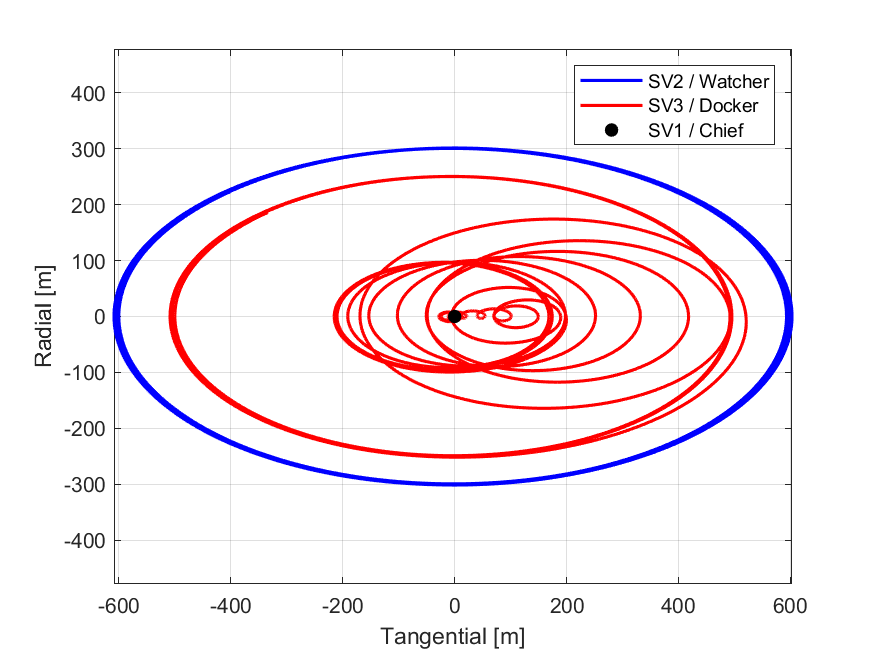
\includegraphics[width=0.5\linewidth]{sim/figures/PS6/RTN_3d_projections_all_maneuvers_cont.png_RT.png}
    \caption{Continuous control modes in RT plane}
    \label{fig:cont_control_RT}
\end{figure}
\begin{figure}[H]
    \centering
    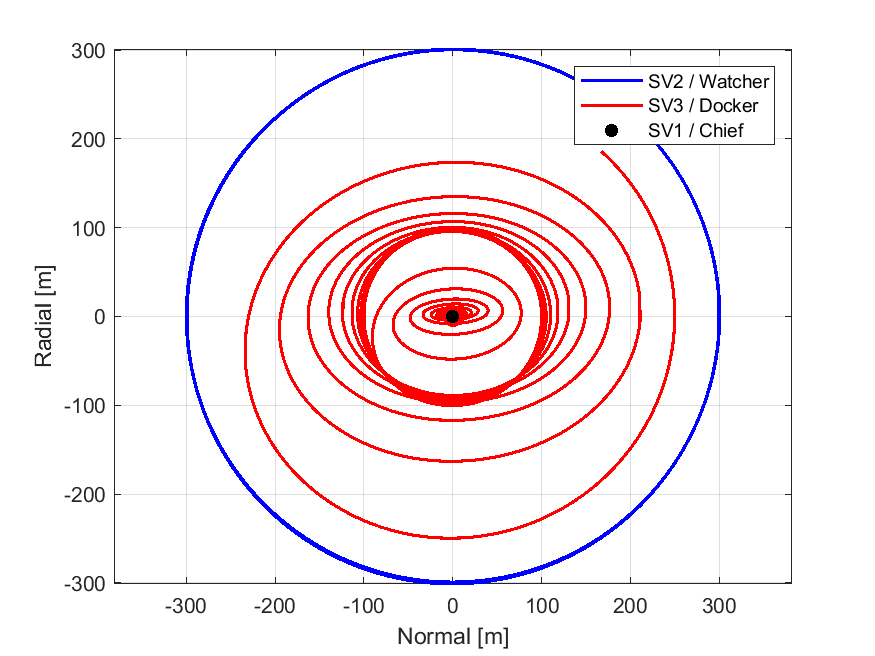
\includegraphics[width=0.5\linewidth]{sim/figures/PS6/RTN_3d_projections_all_maneuvers_cont.png_RN.png}
    \caption{Continuous control modes in RN plane}
    \label{fig:cont_control_RN}
\end{figure}
\begin{figure}[H]
    \centering
    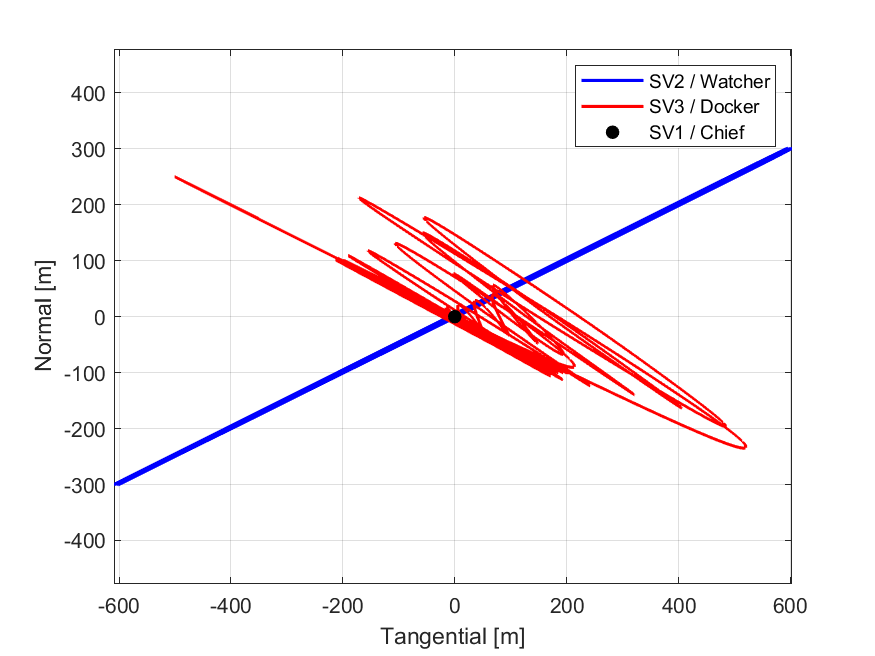
\includegraphics[width=0.5\linewidth]{sim/figures/PS6/RTN_3d_projections_all_maneuvers_cont.png_NT.png}
    \caption{Continuous control modes in NT plane}
    \label{fig:cont_control_NT}
\end{figure}

For SV2, Figures \ref{fig:roe_planes_modes_cont_SV2} and \ref{fig:roe_time_modes_cont_SV2} show the desired and actual ROEs for each mode, which remain constant. The control system tries to keep all ROEs at their initial value. It does so fairly successfully as all ROEs end up within 1 meter of their desired value. These offsets are introduced due to the control system trying to keep $\delta \lambda$ as close to zero as possible through changing $\delta a$ as explain in Section \ref{sec:Lyapunov_implementation}. This has follow on effects on the relative eccentricity and inclination, although they are minor. 

\begin{figure}[H]
    \centering
    \includegraphics[width=0.75\linewidth]{sim/figures/PS6/ROE_planes_modes_SV2.png}
    \caption{Actual and desired ROE plotted for all modes in ROE planes, SV2}
    \label{fig:roe_planes_modes_cont_SV2}
\end{figure}
\begin{figure}[H]
    \centering
    \includegraphics[width=0.75\linewidth]{sim/figures/PS6/ROE_over_time_modes_SV2.png}
    \caption{Actual and desired ROE plotted for all modes in ROE time history, SV2}
    \label{fig:roe_time_modes_cont_SV2}
\end{figure}

The same trends can be seen in the errors plotted in Figure \ref{fig:roe_error_time_modes_cont_SV2}. 
\begin{figure}[H]
    \centering
    \includegraphics[width=0.75\linewidth]{sim/figures/PS6/ROE_error_over_time_modes_SV2.png}
    \caption{Tracking error between actual and desired ROE plotted for all modes in ROE time history, SV2}
    \label{fig:roe_error_time_modes_cont_SV2}
\end{figure}

For SV3, Figures \ref{fig:roe_planes_modes_cont_SV3} and \ref{fig:roe_time_modes_cont_SV3} show the desired and actual ROEs for each mode. $\delta a$ becomes non-zero during the maneuvers because there are along-track elements. The magnitude of $\delta a$ is chosen in order to induce a calculated rate of change in $\delta \lambda$ so that it too can reach a desired value. So $\delta \lambda$ also becomes non-zero during maneuvers, but converges back to zero by the end of the maneuver. This indirect control method is explained at the end of Section \ref{sec:Lyapunov_implementation}. 

$\delta e_x$ and $\delta i_x$ are always meant to be zero, but again the maneuvers introduce variations. Each control mode tries to return $\delta e_x$ and $\delta i_x$ to zero but is unable to get all the way there. These errors can be addressed by allowing for more orbits to converge and more robust station-keeping control in between modes. Right now the continuous station-keeping control is designed to hold the state that it is started at. 

$\delta e_y$ and $\delta i_y$ exhibit the most accurate behavior. The control system is able to reach the desired $\delta e_y$ and $\delta i_y$ in each mode with very little error. This is important because these are the only non-zero factors in the desired ROEs and drive passive safety. 

\begin{figure}[H]
    \centering
    \includegraphics[width=0.75\linewidth]{sim/figures/PS6/ROE_planes_modes_SV3.png}
    \caption{Actual and desired ROE plotted for all modes in ROE planes, SV3}
    \label{fig:roe_planes_modes_cont_SV3}
\end{figure}
\begin{figure}[H]
    \centering
    \includegraphics[width=0.75\linewidth]{sim/figures/PS6/ROE_over_time_modes_SV3.png}
    \caption{Actual and desired ROE plotted for all modes in ROE time history, SV3}
    \label{fig:roe_time_modes_cont_SV3}
\end{figure}

Figure \ref{fig:roe_error_time_modes_cont_SV3} reflects the same behavior in the tracking errors. The control system is able to track all of the desired ROEs very well. The remaining tracking errors can be mitigated either through allowing for more time to converge, adjusting values of $k$ and $N$, or an enhanced station-keeping method. Other methods, such as Lyapunov with constraints or convex optimization, can also be explored, but do not appear to be necessary for the desired behavior in this system. 

\begin{figure}[H]
    \centering
    \includegraphics[width=0.75\linewidth]{sim/figures/PS6/ROE_error_over_time_modes_SV3.png}
    \caption{Tracking error between actual and desired ROE plotted for all modes in ROE time history, SV3}
    \label{fig:roe_error_time_modes_cont_SV3}
\end{figure}

Figure \ref{fig:delta_v_modes_cont_SV3} shows the delta-v magnitudes in the RTN directions throughout each control mode for SV3. By design, there are no radial burns. As expected, individual delta-v magnitudes are similar to impulsive ones in magnitude and are on the scale of mm/s. However, the cumulative delta-v magnitudes for each mode are much larger due to the nature of continuous control. In this implementation, continuous control is broken into impulsive like control for each time step. So, instead of a few delta-v's being applied for the entire control mode, as seen in impulsive control, continuous control has many delta-v's for extended periods of time. These delta-v's are also oscillating as they correct for tracking errors. These characteristics make continuous control exhibit much larger total delta-v than impulsive control. 

The magnitudes decrease in size as the desired change in ROE decreases throughout the modes. Additionally, there are more burns in the normal direction than in the tangential direction. This arises from the fact that inclination maneuvers are much more expensive than eccentricity maneuvers. Since each mode changes relative eccentricity and relative inclination by the exact same magnitude, the inclination maneuver is going to have to be larger. 
\begin{figure}[H]
    \centering
    \includegraphics[width=0.75\linewidth]{sim/figures/PS6/delta_v_cumulative_timeline_modes_SV3.png}
    \caption{Actual delta-v of control maneuvers over time, SV3}
    \label{fig:delta_v_modes_cont_SV3}
\end{figure}

As a point of comparison, the theoretical delta-v lower bound can be calculated as follows:
\begin{align*}
\Delta v_{\text{ecc}} &= \frac{1}{2} \cdot n \cdot a \cdot \left\| \Delta \delta\vec{e} \right\| \\
\Delta v_{\text{inc}} &= n \cdot a \cdot \left\| \Delta \delta\vec{i} \right\| \\
\Delta v_{\text{lb}} &= \sqrt{\Delta v_{\text{ecc}}^2 + \Delta v_{\text{inc}}^2}
\end{align*}
Note that only changes in ROEs were in $\delta e$ and $\delta i$, which is why delta-v lower bound can be calculated as the norm of the along-track and cross-track delta-v's. 

Table \ref{tab:dv_comparison_continuous} compares the total delta-v with the theoretical lower-bound. The actual delta-v's were approximately almost two orders of magnitude larger than the theoretical lower-bound for each mode. This is due to the nature of continuous control with frequent, oscillatory burns as mentioned previously. A greater total delta-v for continuous control is acceptable since a low-thrust engine, such as a Hall Effect Thruster, has much higher specific impulse than a higher-thrust engine, such as a cold-gas thruster, which would likely be used for impulsive control. That being said, the control strategy could be improved to better optimize delta-v and thus fuel usage through the introduction of constraints in the Lyapunov formulation and exploration of convex optimization. 
\begin{table}[H]
\centering
\begin{tabular}{|c|c|c|}
\hline
\textbf{Mode} & \textbf{Total }$\Delta v$ \textbf{(m/s)} & \textbf{Lower Bound (m/s)} \\
\hline
2 & 17.6259 & 0.1830 \\
3 & 10.5896 & 0.1098 \\
4 & 1.0535 & 0.0110 \\
\hline
\end{tabular}
\caption{Total delta-$v$ for continuous control compared with theoretical lower bounds for each maneuver mode}
\label{tab:dv_comparison_continuous}
\end{table}

\newpage
\section{Problem Set 7} \label{sec:7}

\subsection{Recap of Relative Orbital Work}
Over the past two problem sets, we were able to successfully implement two methods of relative orbit control. The first method was using a naive least squares formulation for impulsive control and station keeping. The second method was using a Lyapunov-value function based optimal control method for continuous control, also used for both station keeping and orbital reconfiguration maneuvers. The main takeaways so far are:
\begin{itemize}
    \item The naive-least squares method is sub-optimal, using much more fuel than the lower bound. The benefit of this is that the maneuvers can be completed in a short time-frame. 
    \item Without a thrust constraint and proper tuning of the hyper-parameters, the continuous control uses significantly more $\Delta v$ than the impulsive control methods. The continuous control also requires significantly larger time windows to reach its target.
\end{itemize}
Based on these prior lessons, the next steps would be to use impulsive control, but use a closed-form solution based on reachable set theory that requires less $\Delta v$ than the current naive least-squares implementation. We do not have a requirement on our system for the thrusters we can use, so using continuous control with sub-optimal results and hyperparameter tuning does not make sense. The closed-form control method will be implemented along with the navigation work in Problem Set 8.

The team will also test run a method based on sequential convex optimization, in hopes that that provides a global minimum continuous control policy in terms of fuel usage. If this performs comparably to the impulsive control in terms of thrust (i.e. accounting for the continuous control having a much higher $I_{sp}$), then we may finalize with using SCP-based control.

\subsection{Initial Navigation System Design}

\subsubsection{Choice of State Representation} \label{sec:nav_state_rep}
We will be using an Extended Kalman Filter (EKF) for our navigation system. Within the EKF, we will use a mixed state representation of absolute and relative orbit elements of the chief and deputies. Specifically, we will estimate the absolute orbit elements of the chief and the relative orbit elements of the deputy. The resulting state vector is:

\begin{equation}
\begin{bmatrix}
\boldsymbol{\alpha}_1 \\
\hline
\delta \boldsymbol{\alpha}_2 \\
\hline
\delta \boldsymbol{\alpha}_3
\end{bmatrix}
=
\begin{bmatrix}
a_1 \\
e_{x,1} \\
e_{y,1} \\
i_1 \\
\Omega_1 \\
u_1 \\
\hline
\delta a_2 \\
\delta \lambda_2 \\
\delta e_{x,2} \\
\delta e_{y,2} \\
\delta i_{x,2} \\
\delta i_{y,2} \\
\hline
\delta a_3 \\
\delta \lambda_3 \\
\delta e_{x,3} \\
\delta e_{y,3} \\
\delta i_{x,3} \\
\delta i_{y,3}
\end{bmatrix}
\end{equation}

This state representation was chosen because we are not assuming perfect knowledge of the absolute chief state, so we must estimate it. This estimated absolute chief state then informs our estimation of the relative states of the deputies, which are inherently the focus of our docking and servicing mission. Orbit elements in general were chosen because they give more immediately intuitive understandings of the relative state and change much less rapidly then Cartesian position and velocity do. This makes it easier for our filter to accurate estimate the state since the magnitude of propagation steps is smaller. 

\subsubsection{Dynamics Model for State Prediction}
For predicting the state within the filter, two different dynamics models will be used. For predicting the absolute chief orbit elements, the nonlinear Gauss Variational Equations (GVEs) will be numerically integrated. This approach is outlined in Section \ref{sec:osc_mean_J2}. For predicting the relative orbit elements of the deputies, the ROEs will be propagated via numerical integration of the following expression from Koenig \cite{koenig2017new}:

\begin{equation}
\delta \dot{\boldsymbol{\alpha}_{\text{qns}'}} = 
\kappa_d
\begin{pmatrix}
0 \\
\eta_d(3\cos^2 i_d - 1) + (5\cos^2 i_d - 1) - 2\cos i_d \cos i_c \\
- e_d \sin(\omega_d - \omega_c)(5\cos^2 i_d - 1) \\
e_d \cos(\omega_d - \omega_c)(5\cos^2 i_d - 1) \\
0 \\
-2\cos i_d \sin i_c
\end{pmatrix}
-
\kappa_c
\begin{pmatrix}
0 \\
(1 + \eta_c)(3\cos^2 i_c - 1) \\
- e_d \sin(\omega_d - \omega_c)(5\cos^2 i_c - 1) \\
e_d \cos(\omega_d - \omega_c)(5\cos^2 i_c - 1) \\
0 \\
-2\cos i_c \sin i_c \\
\end{pmatrix}
\label{eq:ROE_nonlinear}
\end{equation}

where:
\begin{align*}
\eta_d &= \sqrt{1 - e_d^2} \\
\eta_c &= \sqrt{1 - e_c^2} \\
\\
\kappa_d &= \frac{3 J_2 R_E^2 \sqrt{\mu}}{4 a_d^{7/2} \eta_d^4} \\
\kappa_c &= \frac{3 J_2 R_E^2 \sqrt{\mu}}{4 a_c^{7/2} \eta_c^4}
\end{align*}

This expression is the non-linear time derivative of the modified ROE, and thus can be used for propagation. Note that this expression uses the modified ROEs to obtain a more sparse plant matrix. The modified ROEs are defined as:
\begin{equation}
\delta \boldsymbol{\alpha}_{\text{qns}'} = \mathbf{J}_{\text{qns}}(\alpha_c) \, \delta \boldsymbol{\alpha}_{\text{qns}}
\end{equation}

where:
\begin{equation}
\mathbf{J}_{\text{qns}}(\alpha_c) =
\begin{bmatrix}
\mathbf{I}_{2 \times 2} & \mathbf{0}_{2 \times 2} & \mathbf{0}_{2 \times 2} \\
\mathbf{0}_{2 \times 2} & 
\begin{bmatrix}
\cos \omega & \sin \omega \\
-\sin \omega & \cos \omega
\end{bmatrix}
& \mathbf{0}_{2 \times 2} \\
\mathbf{0}_{2 \times 2} & \mathbf{0}_{2 \times 2} & \mathbf{I}_{2 \times 2}
\end{bmatrix}
\end{equation}

and where the modified ROE are defined as:
\begin{equation}
\delta \boldsymbol{\alpha}_{\text{qns}'} =
\begin{pmatrix}
\delta a \\
\delta \lambda \\
\delta e_{x'} \\
\delta e_{y'} \\
\delta i_x \\
\delta i_y
\end{pmatrix}
=
\begin{pmatrix}
\frac{a_d - a_c}{a_c} \\
(M_d - M_c) + (\omega_d - \omega_c) + (\Omega_d - \Omega_c) \cos i_c \\
e_d \cos(\omega_d - \omega_c) - e_c \\
e_d \sin(\omega_d - \omega_c) \\
i_d - i_c \\
(\Omega_d - \Omega_c) \sin i_c
\end{pmatrix}
\end{equation}

Using these expressions, we can propagate ROE for each discrete time step, transforming from quasi-nonsingular ROE to modified quasi-non-singular ROE appropriately. This propagation only takes into account Keplerian and J2 effects and does not include control inputs. 

To propagate with control inputs, the control input matrix defined by Chernick is used \cite{chernick2021optimal}:
\begin{equation}
\Delta \delta \boldsymbol{\alpha}_k = \boldsymbol{\Gamma}_k \delta \mathbf{v}_k = 
\frac{1}{n a}
\begin{bmatrix}
0 & 2 & 0 \\
-2 & 0 & 0 \\
\sin(u_k) & 2 \cos(u_k) & 0 \\
-\cos(u_k) & 2 \sin(u_k) & 0 \\
0 & 0 & \cos(u_k) \\
0 & 0 & \sin(u_k)
\end{bmatrix}
\begin{bmatrix}
\delta v_R \\
\delta v_T \\
\delta v_N
\end{bmatrix}
\label{eq:control_input_matrix}
\end{equation}

At every discrete time step, the filter prediction step checks to see if there is a control input. If there is an applied delta-v then the above expression is used to find the instantaneous change in ROE, which is added to the current ROE state. This state is then propagated using Equation \ref{eq:ROE_nonlinear}. 

This nonlinear filter propagation method was chosen to attain high accuracy as compared to the STM, which is a first-order Taylor series approximation of the nonlinear Equation \ref{eq:ROE_nonlinear}. The linearized STM is usually sufficient for small separations in $\delta a$, $\delta e_x$, $\delta e_y$, and $\delta i_x$, and arbitrary separations in $\delta \lambda$ and $\delta i_y$. \cite{koenig2017new} But for utmost accuracy, which is required in rendezvous and docking, nonlinear propagation captures higher-order behavior. 

The ground truth is also propagated using nonlinear equations, but these are in the ECI frame. Thus nonlinear propagation in ROEs was chosen to differentiate the filter prediction from the ground truth. In further work, the ground truth can also be enhanced through the addition of other perturbations such as drag. Additionally, different values of noise can be added to the ground truth and filter to further differentiate them. Another difference is in the integration methods. The filter uses Euler integration as opposed to Runge Kutta integration which the ground truth uses. The Euler integration is used because it is computationally less expensive and provides more distinction from the ground truth. 

The ROE nonlinear propagation was verified by comparing it to the ground truth, as seen in Figure \ref{fig:ROE_nonlinear_compare}. 

\begin{figure}[H]
    \centering
    \includegraphics[width=0.75\linewidth]{sim/figures/PS7/ROE_over_time_SV3_comparison.png}
    \caption{ROE over time comparison for SV3}
    \label{fig:ROE_nonlinear_compare}
\end{figure}

The EKF Mean Propagation method aligns well with the ground truth for a propagation with no control inputs, showcasing J2 effects on $\delta e_x$ and $e_y$. In fact, it exhibits better behavior than the ground truth, since it has zero $\delta a$ and $\delta i_x$, which also means there is no $\delta \lambda$ or $\delta i_y$ drift from J2. The ground truth exhibits these drifts because of numerical error in the conversion from osculating to mean quantities that leads to nonzero $\delta a$ and $\delta i_x$, and an initial offset in $\delta e_x$. As such, the EKF Mean Propagation method is verified to be accurate. The ground truth propagation should be improved to remove the unexpected behavior it exhibits. 

\subsubsection{Linearized Dynamics Model for Covariance Update}
The dynamics models are linearized and then applied to the covariance update in the EKF.  

For the chief absolute orbit elements, the J2-induced secular drift rates with Keplerian motion added are:

\begin{align}
\frac{d e_x}{d t} &= -\frac{3}{4} n J_2 \left( \frac{R_E}{a \left( 1 - (e_x^2 + e_y^2) \right)} \right)^2 e_y (5 \cos^2 i - 1) \\
\frac{d e_y}{d t} &= \phantom{-}\frac{3}{4} n J_2 \left( \frac{R_E}{a \left( 1 - (e_x^2 + e_y^2) \right)} \right)^2 e_x (5 \cos^2 i - 1) \\
\frac{d \Omega}{d t} &= -\frac{3}{2} n J_2 \left( \frac{R_E}{a \left( 1 - (e_x^2 + e_y^2) \right)} \right)^2 \cos i  \\
\frac{d u}{d t} &= n + \frac{3}{4} n J_2 \left( \frac{R_E}{a \left( 1 - (e_x^2 + e_y^2) \right)} \right)^2 \left[ \sqrt{1 - (e_x^2 + e_y^2)} (3 \cos^2 i - 1) + (5 \cos^2 i - 1) \right] 
\end{align}

To get the STM, we now compute the Jacobian matrix \( \mathbf{A} = \partial \dot{\boldsymbol{\alpha}} / \partial \boldsymbol{\alpha} \) using first-order partials.

Let \( e^2 = e_x^2 + e_y^2 \), \( \eta = \sqrt{1 - e^2} \), and

\[
K = \frac{3}{4} n J_2 \left( \frac{R_E}{a(1 - e^2)} \right)^2
\]

Derivatives of \( \dot{e}_x \):
\[
\frac{\partial}{\partial e_y} \left( \frac{d e_x}{dt} \right) = -K (5 \cos^2 i - 1), \quad
\frac{\partial}{\partial i} \left( \frac{d e_x}{dt} \right) = -10 K e_y \cos i \sin i
\]

Derivatives of \( \dot{e}_y \):
\[
\frac{\partial}{\partial e_x} \left( \frac{d e_y}{dt} \right) = K (5 \cos^2 i - 1), \quad
\frac{\partial}{\partial i} \left( \frac{d e_y}{dt} \right) = 10 K e_x \cos i \sin i
\]

Derivative of \( \dot{\Omega} \):
\[
\frac{\partial}{\partial i} \left( \frac{d \Omega}{dt} \right) = 2K \sin i
\]

Derivatives of \( \dot{u} \):

\[
\frac{d u}{dt} = n + K \left[ \eta (3 \cos^2 i - 1) + (5 \cos^2 i - 1) \right]
\]

Partial w.r.t. \( e_x \):

\[
\frac{\partial \eta}{\partial e_x} = \frac{-e_x}{\eta}, \quad
\frac{\partial}{\partial e_x} \left( \frac{du}{dt} \right) = -K (3 \cos^2 i - 1) \cdot \frac{e_x}{\eta}
\]

Partial w.r.t. \( e_y \):

\[
\frac{\partial}{\partial e_y} \left( \frac{du}{dt} \right) = -K (3 \cos^2 i - 1) \cdot \frac{e_y}{\eta}
\]

Partial w.r.t. \( i \):

\[
\frac{\partial}{\partial i} \left( \frac{du}{dt} \right)
= K \cdot \frac{d}{di} \left[ \eta (3 \cos^2 i - 1) + (5 \cos^2 i - 1) \right]
= -6 K \cos i \sin i \left( \eta + \tfrac{5}{3} \right)
\]

Finally, putting all the partials together:

\[
\mathbf{A} =
\begin{bmatrix}
0 & 0 & 0 & 0 & 0 & 0 \\
0 & 0 & -K(5\cos^2 i - 1) & -10 K e_y \cos i \sin i & 0 & 0 \\
0 & K(5\cos^2 i - 1) & 0 & 10 K e_x \cos i \sin i & 0 & 0 \\
0 & 0 & 0 & 0 & 0 & 0 \\
0 & 0 & 0 & 2K \sin i & 0 & 0 \\
0 & -K(3 \cos^2 i - 1) \frac{e_x}{\eta} &
    -K(3 \cos^2 i - 1) \frac{e_y}{\eta} &
    -6K \cos i \sin i \left( \eta + \tfrac{5}{3} \right) & 0 & 0
\end{bmatrix}
\]

Then, the linearized STM for the absolute chief orbit elements is:

\[
\Phi(t, t_0) \approx \mathbf{I} + \mathbf{A} \, \Delta t
\]

For the relative orbit elements, the STM is given by \ref{eq:stm_matrix}. Together, these two STMs will be used to update covariance in the EKF. The control input matrix is given by Equation \ref{eq:control_input_matrix} is only relevant for the relative deputy states since the chief is not under control. Additionally, it is not dependent on the relative orbit elements state so it will not appear in the linearized covariance update equation. 

\subsubsection{On-board Sensors and Measurements}

Each of the deputies (SV2 and SV3) is equipped with the following sensors, which also give the raw measurements mentioned below:
\begin{itemize}
    \item \textbf{Vision-based sensors:} These provide relative bearing angle measurements for SV2 and SV3 relative to SV1. We assume that the sensors on SV2 and SV3 are always pointed at SV1. For close-range measurements required during SV3's docking phase, the vision-based sensors can also provide feature-rich images that may be used for more accurate position estimation. 
    \item \textbf{GNSS antennas:} These provide GNSS measurements such as pseudoranges. For simplicity, we stick with the single-difference GNSS pseudoranges. Although, in the future, we will consider combing the pseudo-range measurements get to apply double-difference GNSS methods.
\end{itemize}

These raw measurements can be converted into simpler pseudo-measurements based on standard operations for each of the sensors. 
\begin{itemize}
    \item The relative bearing angle measurements of the vision-based sensor, $\alpha$ and $\epsilon$, can be converted into relative position vector measurements in the rectilinear frame $\boldsymbol{x}^\mathcal{R}$ \cite{sullivan2020nonlinear}. For this project, we make the simplifcation that the vision-based sensor gives us the pseudo-measurement of the relative position vector of the deputy in the chief's RTN frame.
    \item The psuedorange measurements acquired from the GNSS signals can be converted into absolute position measurements for the deputy satellites. For this project, we make the simplifcation that the GNSS sensors give us the psuedo-measurement of the absolute positions of the deputies in the ECI frame.
\end{itemize}
These pseudo-measurements are compiled into a measurement vector $y_{SV}$, for each spacecraft. For SV2, this is given by

\begin{align}
    y_{SV2} = \begin{bmatrix}
        \boldsymbol{r_{SV2}}^{RTN}\\
        \boldsymbol{x_{SV2}}^{ECI}
    \end{bmatrix}_{6\times 1}
\end{align}

A similar measurement vector $y_{SV3}$ is built for SV3. The combined full measurement vector, for both spacecraft together, is given by

\begin{align}
    y &= \begin{bmatrix}
        y_{SV2} \\
        y_{SV3}
    \end{bmatrix} \\
    &= \begin{bmatrix}
        \boldsymbol{r_{SV2}}^{RTN}\\
        \boldsymbol{r_{SV2}}^{ECI} \\
        \boldsymbol{r_{SV3}}^{RTN} \\
        \boldsymbol{r_{SV3}}^{ECI} \\
    \end{bmatrix}_{12\times 1}
\end{align}

An important note here is that although the chief's orbital elements are part of the state we are estimating, since the chief (SV1/Target) is not under active control and is a rogue spacecraft that we want to dock with, we do not receive any measurements specific to SV1. It is imperative, however, for us to have an estimate of SV1's motion to make sense of the absolute and relative measurements of SV2 and SV3.

For the purposes of this project, these measurements will just be noisy versions of the true states, with some added Gaussian noise. As such, no unit testing is required at this step.

\subsubsection{Measurement Model}
The measurement model relates the pseudo-measurements in $y$ from the vision-based sensors and the GNSS antennas to the state of the spacecrafts $x$, by some non-linear function $g(\cdot)$, i.e.
\begin{align}
    y_{SV2} &= g_{SV2}(\alpha_{1}, \delta \alpha _{2}) \\
    y_{SV3} &= g_{SV3}(\alpha_{1}, \delta \alpha _{2}) \\
    y &= g(x)
\end{align}

Here, $g(x):\mathbb{R}^{18} \rightarrow \mathbb{R}^{12}$ is a simple concatenation of each $g_{SV2}(\cdot)$ and $g_{SV3}(\cdot)$. For the selected pseudo-measurements, the measurement model we have converts our state-space representation that includes the chief's orbital elements and the deputy spacecraft's relative orbital elements into the pseudo-measurements of relative and absolute position vectors.

The conversion from relative orbital element to relative position vectors can be done in a non-linear fashion with higher fidelity by intermediately converting to absolute orbital elements, to ECI, and then to RTN. However, as shown in Chapter 2 of \cite{damicothesis}, for near-circular orbits we can find a linear mapping between the quasi-nonsingular relative orbital elements and position and velocity in the RTN frame (by relating the relative orbital elements to the integration constants in the Hill-Clohessy-Wiltshire equations). This is given by
\begin{align}
\boldsymbol{r}^{RTN} &\approx a_1
\begin{bmatrix}
1 & 0 & -\cos u_1 & -\sin u_1 & 0 & 0 \\
0 & 1 & 2\sin u_1 & -2\cos u_1 & 0 & 0 \\
0 & 0 & 0 & 0 & \sin u_1 & -\cos u_1 \\
\end{bmatrix}
\delta \boldsymbol{\alpha} \\
\boldsymbol{r}^{RTN} &\approx 
\mathcal{J}
a_1\delta \boldsymbol{\alpha} \\
\end{align}
where $u$ is the mean argument of latitude of the chief spacecraft. We use $\mathcal{J}_{3\times 6}$ to represent this transformation matrix. This is linear with respect to the deputy, but non-linear with respect to the chief's state.

The conversion from relative orbital elements to absolute position vectors can be done by converting to approximate RTN values as before, and then performing a rotation from relative RTN positions to ECI positions. The chief's ECI state is required here, which can also be converted from the chief's orbital elements.
\begin{align}
    \boldsymbol{r}^{ECI} = Q^\top_{eci2rtn} \boldsymbol{r}^{RTN} + \boldsymbol{r}_{SV1}^{ECI}
\end{align}
where $Q^\top_{eci2rtn}$ is defined using $\boldsymbol{r}_{SV1}^{ECI}$, as described in Equation \ref{eq:v_rtn_rel}. The calculation of $\boldsymbol{r}_{SV1}^{ECI}$ is itself a non-linear function of the chief's orbital elements, which is described in detail in Section \ref{sec:initial_ECI}. We can call this function $f_{oe2eci}(\cdot)$
\begin{align}
    \boldsymbol{r}_{SV1}^{ECI} = f_{oe2eci}(\boldsymbol{\alpha}_1)
\end{align}
With all these elements, we can now represent the measurement model and the relation between the state defined in Section \ref{sec:nav_state_rep} to our measurement vector.
\begin{align}
    y = &g(x) \\
    &g(x) = \begin{bmatrix}
        \mathcal{J}
a_1\delta \boldsymbol{\alpha}_2 \\
            Q^\top_{eci2rtn} \mathcal{J}
a_1\delta \boldsymbol{\alpha}_2 + f_{oe2eci}(\boldsymbol{\alpha}_1) \\
        \mathcal{J}
a_1\delta \boldsymbol{\alpha}_3 \\
            Q^\top_{eci2rtn} \mathcal{J}
a_1\delta \boldsymbol{\alpha}_3 + f_{oe2eci}(\boldsymbol{\alpha}_1) \\
    \end{bmatrix}_{12\times 1}
\end{align}

Since we are making some linear approximations in our measurement model, we plan on setting up some unit test cases to make sure this measurement model tracks. The unit test will verify that the measurement model aligns to some error tolerance (larger than the expected added noise) with the true measurements. If the residual between the measurements and the measurement model increases in any of the unit tests, then there is a case where the measurement model breaks down. The unit tests will help identify what these cases are, and where the measurement model might need improvements.

\subsubsection{Sensitivity Matrix}

The sensitivity matrix $C_t$ is formed by taking the Jacobian of the nonlinear function $g(x)$ with the current state value $x_t$. This gives us the linearized relation between the state vector $x_t$ and the measurement vector $y_t$.
\begin{align}
    y_t = C_tx_t\\
    C_t = \left . \frac{\partial g}{\partial x} \right|_{x = \bar{x}_t}
\end{align}

Taking the Jacobian, we get a matrix of dimensions $12 \times 18$. $C_t$ will be of the form
\begin{align}
    C_t = \left.\begin{bmatrix}
        \dfrac{\partial \mathcal{J}a_1 \delta \boldsymbol{\alpha}_2}{\partial \boldsymbol{\alpha}_1}  & \mathcal{J}a_1 & 0_{3\times6} \\
        \dfrac{Q^\top_{eci2rtn} \mathcal{J}
a_1\delta \boldsymbol{\alpha}_2 + f_{oe2eci}(\boldsymbol{\alpha}_1)}{\partial \boldsymbol{\alpha}_1} & Q^\top_{eci2rtn} \mathcal{J}
a_1 & 0_{3\times6} \\
        \dfrac{\partial \mathcal{J}a_1 \delta \boldsymbol{\alpha}_3}{\partial \boldsymbol{\alpha}_1}  & 0_{3\times6}  & \mathcal{J}a_1 \\
        \dfrac{Q^\top_{eci2rtn} \mathcal{J}
a_1\delta \boldsymbol{\alpha}_3 + f_{oe2eci}(\boldsymbol{\alpha}_1)}{\partial \boldsymbol{\alpha}_1} & 0_{3\times6} & Q^\top_{eci2rtn} \mathcal{J}
a_1\\
    \end{bmatrix} \right|_{x = \bar{x}_t}
\end{align}
The Jacobian is evaluated with $\bar{x}_t$, i.e. the value of the state at time $t$. This makes $C_t$ time-varying. In an Extended Kalman Filter, this sensitivity matrix $C_t$ is used to find the Kalman gain and thus update the state covariance estimate.

The inclusion of SV1's position in the state greatly complicates the calculation of the sensitivity matrix $C$. If this becomes restrictive when implementing the Kalman filter, then we may consider assuming perfect state knowledge of SV1, and only estimating the states of the deputies. 

It is critical that this formulation of the sensitivity matrix remain observable. Therefore, the unit tests here will check the condition number of the observability matrix over time for different short simulations, to ensure that the system is observable and the covariance of the state can be estimated.








%%%%%%%%%%%%%%%%%%%%%%%%%%%%%%%
% REFERENCES
%%%%%%%%%%%%%%%%%%%%%%%%%%%%%%%
\newpage
\section{References}
\printbibliography[heading=none]

%%%%%%%%%%%%%%%%%%%%%%%%%%%%%%%
% APPENDIX 1: CODE
%%%%%%%%%%%%%%%%%%%%%%%%%%%%%%%
\newpage
\appendix
\section{Appendix: Code}

% Optional: Git repository link to your code
% All code for this project can be found in the following \href{}{Git repository}.

\subsection{Problem Set 1 Code}

Code is available at our GitHub: \href{https://github.com/GigaVoltFlash/AA279D}{https://github.com/GigaVoltFlash/AA279D}.

Refer to \href{https://github.com/GigaVoltFlash/AA279D/blob/main/sim/sim_main.m}{sim\_main.m} as the main file where we run our sim.


\end{document}